\documentclass[a4paper]{article}
\usepackage[top=0.75in, bottom=0.5in, left=1in, right=1in]{geometry}
%\usepackage[titletoc]{appendix}
\usepackage{times}
\usepackage{amsmath}
\usepackage{amssymb}
\usepackage{mathrsfs}
\usepackage{natbib}
\usepackage{aas_macros}
\usepackage{fancyvrb}
\usepackage{gensymb}
\usepackage{appendix}
\usepackage{multirow}
\usepackage{longtable}
\usepackage{caption}
\usepackage[UKenglish]{datetime}

% Graphics type
\usepackage[pdftex]{graphicx}

\newcommand\prox{Proxima Centauri}
\newcommand\bstar{Barnard's Star}
\newcommand\rdwarf{M-dwarf}
\newcommand\ldwarf{L-dwarf}
\newcommand{\bvec}[1]{\mbox{\boldmath ${#1}$}}
\newcommand{\rmsub}[2]{#1_{\rm #2}}
\newcommand{\dex}[1]{\hbox{$\times\hbox{10}^{#1}$}}
\newcommand{\rsun}{\,\mbox{$\rm R_{\odot}$}}
\newcommand{\rjup}{\,\mbox{$\rm R_J$}}
\newcommand{\msun}{\,\mbox{$\rm M_{\odot}$}}
\newcommand{\mearth}{\,\mbox{$\rm M_{\oplus}$}}
\newcommand{\mjup}{\,\mbox{$\rm M_J$}}
\newcommand{\lsun}{\,\mbox{$\rm L_{\odot}$}}
\newcommand{\ion}[2]{#1{\sc{\romannumeral #2}}}
\newcommand{\chem}[2]{\hbox{$^{#2}$}#1}
\newcommand{\kms}{\hbox{kms$^{-1}$}}
\newcommand{\ms}{\hbox{ms$^{-1}$}}
\newcommand{\cms}{\hbox{cms$^{-1}$}}
\newcommand{\vsini}{\hbox{$v$\,sin\,$i$}}
\newcommand{\vs}{\hbox{$v$\,sin\,$i$}}
\newcommand{\rsini}{\hbox{$R$\,sin\,$i$}}
\newcommand{\vrad}{\hbox{$v_{rad}$}}
\newcommand{\degs}{$\degr$}
\newcommand{\chisq}{$\chi^{2}$} 
\newcommand{\radsec}{rad s$^{-1}$}
\newcommand{\radday}{\hbox{rad.day$^{-1}$}}
\newcommand{\invday}{\hbox{day$^{-1}$}}
\newcommand{\ha}{H$\alpha$}
\newcommand{\hb}{H$_{\beta}$}
\newcommand{\hg}{H$_{\gamma}$}
\newcommand{\hd}{\hbox{HD 189733}}
\newcommand{\hdb}{\hbox{HD 189733b}}
\newcommand{\dom}{\hbox{$\Delta\Omega$}}
\newcommand{\tps}{\hbox{$T_{p}/T_{s}$}}

\newcommand{\eev}{{\sc eev}}
\newcommand{\mitll}{{\sc mitll}}
\newcommand{\harps}{{\sc harps}}
\newcommand{\asas}{{\sc asas}}
\newcommand{\uves}{{\sc uves}}
\newcommand{\vlt}{{\sc vlt}}
\newcommand{\hst}{{\sc hst}}

\newcommand{\scipy}{{\sc scipy}}
\newcommand{\astroml}{{\sc astroml}}
\newcommand{\gatspy}{{\sc gatspy}}
\newcommand{\matplot}{{\sc matplotlib}}

% So we can change our minds what to call them

\newcommand{\horn}{sub-peak}

\newcommand\Notnow[1]{}

% Stuff different between paper and thesis, this is for paper
% ===========================================================

\newcommand\IfPaper[1]{#1}
\newcommand\IfThesis[1]{}
\newcommand\PaperThesis[2]{#1}
\newcommand\paperorthesis{freport}
\newcommand\FirstP{We}
\newcommand\Firstp{we}
\newcommand\Firstobj{us}
\newcommand\Firstposs{our}
\newcommand\FirstPoss{Our}

\newdateformat{engwithth}{\ordinal{DAY}~\monthname[\THEMONTH] \THEYEAR}
\newdateformat{engdate}{\THEDAY~\monthname[\THEMONTH] \THEYEAR}
\newdateformat{monthonly}{\monthname[\THEMONTH] \THEYEAR}

\begin{document}

\title{Analysis of Red Dots project REM observations of 3 {\rdwarf}
objects}

\author{John M. Collins\\
  University of Hertfordshire,\\
  College Lane, Hatfield, Herts, \\
  AL10 9AB, UK\\
  \texttt{j.m.collins@herts.ac.uk}\\
  }
\engwithth
\date{\today}
\maketitle

\protect\label{firstpage}

\begin{abstract}

  This report considers the automatic REM observations taken by the Red Dots
  Project of three {\rdwarf} objects, specifically \prox, {\bstar} and Ross 154,
  with particular attention to \bstar. The available data is considered and an
  analysis of the likely precision of measurements suitable for further analysis
  assessed.
  
\end{abstract}

%\keywords{stars: (Proxima Centauri) --- methods: data analysis --- techniques: periodograms --- accuracy}

\section{Introduction}
\protect\label{section:intro}

\engdate

This report is an analysis of the observational data from the REM (Rapid Eye
Mount) camera in La Silla, Chile, operated by the Red Dots Project, This work
commencing in March 2015. \footnote{See \texttt{https://reddots.space/}}. In
this project a series of observations are made of a patch of sky in the vicinity of particular target using four visual
light filters on the ROS2 telescope and 3 infrared filters on the REMIR
telescope. The images from the visbile light telescope are 1024 by 1-24 pixels, although
the effective area is only 900 by 900 and the images from the infrared are 512
by 512 pixels. In each case a 16-bit CCD records the counts for exach pixel.
Flat field and bias frames are only available for the visible light cases.

The primary targets are \rdwarf s, although observations are made of other types
of star during the course of each night.In this report, only the {\rdwarf} observations are considered and only the
visible light cases.

\subsection{Targets}

The three main targets of the REM observations are \prox, {\bstar} and Ross 154,
all \rdwarf s of spectral types M6, M4 and M3.5 respectively and 4.2, 6 and 9.6
ly distant, putting them at nearest, fourth nearest and eleventh nearest known
stellar objects to the solar system.The main subject of study is the
identification of periodic signals in the light curves.

\subsubsection{\prox}
{\prox} is of perennial interest as the closest star to the solar system, at 4.2 ly. It is of spectral type M5.5.
Despite the interest and available data, calculations of the the rotation period
of {\prox} have varied over the years.  Studies have reported periods
ranging from the $ 31.5 \pm 1.5 $ days of \citet{guinan96}, the 41.3 days of \citet{benedict93}
and s between 82 and 84 days in \citealt{benedict92,benedict98}.  \citet{kurster99} found that the period is not less
than 50 days, whilst more recently \citet{kiraga07} reported a value of 82.5
days. All these estimates were based on photometric measurements \citet[Table 3]{suarezmascareno15} reported a value of 116.6 days, using a
measurement of {\ha}. In \citet{collins17} the rotation periods was calculated
ast 82.6 $\pm$ 0.1 days, based primarily on photometric evidence, with some
support from spectroscopic analysis of an {\ha} peak.

In 2016 a planet of 1.3 Earth mass was reported in the habitable
zone of \prox, known as {\prox} b. \citep{angladaescude16}. Its orbital period was calculated as just over 11
days. The following year further studies have suggested dust belts \citep{anglada17} but yet furhter
studies have suggested that a large flare affected those results \citep{macgregor18}.

THe frequent flare activity is unusual in a star of slow rotation like \prox,
previous studies such as In \citet{mohanty03} setting out the correlation
between the projected otational velocity {\vsini} and the
activity in mid-M to L-dwarfs, In \citet{vida19} the flaring activity was
calculated as 1.49 events per day. with ``superflares'' approximately 3 times a
year and flares a magntude larger every other year.

Such frequent flaring, as well as compromising the habitability of {\prox} b,
is clearly likely to interfere with measurements of periodicity. It is highly
likely that many of the observations of {\prox} analysed here are affected by
flares.

Together with the rest of the Alpha Centauri system, the age of {\prox} has been
estimated at $5.26 \pm 0.95$ Gyr, slightly older than the Sun \citep{joyce18}.

As shown in Table \ref{table:obstargets}, the bulk of the observations taken
by the Red Dots project are of \prox.

\subsubsection{\bstar}
{\bstar} is, at just under 6ly, the fourth closest star to the solar system after {\prox} and Alpha Centauri A and B. It is of spectral type M4.
It is particularly notable for its very large proper motion of −802.803 mas/yr in Right Ascension and 10,362.542 mas/yr in Declination., the largest of all
stars relative to the solar system. This is combined with a high radial velocity of $-110.6$ km/s \citep{bobylev17}.
The high radial velocity of {\bstar} will bring it close enough
to the solar system to rival or perhaps surpass {\prox} in approximatelyr 10,000 years as estimated by \citet{bobylev10}.
Its rotation period has been progressively given as 130 days in
\citet{benedict98}, 148.6 days in \citet{suarezmascareno15} and 145 $\pm$ 15 days in \citet{toledopadron18}. Activity is low, as noted in the latter.
It has an estimated age of between 7 to 10 Gyr \citep{ribas18}.

\monthonly
\newdate{firstbs}{1}{8}{2017} 

{\bstar} is of particular interest at the moment, following the announcement of
a planet companion, also noted in \citet{ribas18}, and this report has focused
upon it, espacially as the low activity reduces interference from that source
with periodicity calculations.
Of the observations listed in Table \ref{table:filtersnums}, the corresponding observations for {\bstar} are listed in Table \ref{table:bstarsumm}. Observations were taken between August 2017 and
\date{\today}. Due to the high proper motion, care has to be taken to correctly take this into account when identifying it in images.

\begin{table}[!htbp]
\begin{center}
\begin{tabular}{lr} \hline
Filter & Number \\\hline
g & 1,415 \\
i & 1,414 \\
r & 1,414 \\
z & 1,415 \\
H & 2,264 \\
J & 5,557 \\
K & 2,130 \\
\hline
\end{tabular}
\end{center}
\caption{List of observations to date of \bstar. All were made between
\displaydate{firstbs} and \date{\today}}.
\protect\label{table:bstarsumm}
\end{table}
\engdate

\subsubsection{Ross 154}
Ross 154 is 9.6 ly distant, of spectral type M3.5. It has a reasonably high
proper motion of −+637.02 mas/yr in Right Ascension and  –191.64 mas/yr in
Declination and a radial velocity of –10.7 km/s \citep{vanleeuwen07}.

The strong activity is noted in \citet{wargelin08}. Previously, in
\citet{jarrett76}, an activity cycle of about 2 days was reported.

Nowhere reports a rotation period, however a maximum figure for the rotation
period of $3.5 \pm 1.5$ days can be calculated from the rotational
velocity (\vsini) of $5 \pm 1.5$ km/s fiven in \citet{wargelin08} and the radius of 0.24 solar given in
\citet{johnson83}. If the inclination is other than 90\degree the rotation
period will be shorter by a factor of the sine of the inclination angle.
It would be useful to obtain a figure for the rotation period as no planets have
been reported for Ross 154 and a low inclination angle might be one of the
reasons.

\citet{wargelin08} also state that the fast rotation period is indicative of a
n age of less than 1 Gyr.


\section{Data provided by REM observations}
\protect\label{section:tdataprovided}

\subsection{Data Available}

Consideration of the data available from the Red Dots project site is
hereinafter restricted to the targets of the project, the {\rdwarf} stars,
\prox, {\bstar} and \ross. The relevant data available is.

\begin{itemize}
 \item Images taken with visible light filters \textbf{g},
\textbf{i}, \textbf{r} and \textbf{z} taken almost daily. although not
necessarily of the REM {\rdwarf} targets, especially during April through to the
first part of July each year when the position of the Sun in the sky makes
observations impossible. All the images of the REM {\rdwarf} targets are taken
at a gain of 1 and the other targets with a gain of 4.4. 
\item Sky flat file images taken almost every day, usually as 3 images from the
sky, taken as the light fades. A set is taken with a gain of 4.4 and with a gain
of 1 each time, even if no observations are taken with that gain.
\item Bias file images taken each day
approximately 8 hours after the observations.
\item There are a very small number of dark file images (as for bias but with
an exposure of other than zero) taken in 2015, but these were from two years
before before the {\rdwarf} observations were commenced and are disregarded
herein.
\item Monthly master flat file images for each month constructed from some of
the daily flat files for the month in question.
\item Monthly master bias file images for each month, constructed from some of
the daily bias files for the month in question.
\item REMIR infrared images taken almost every day up to June 2019. These are
already reduced with the PREPROCESS software \citep{dipaola01}.
\item IDL routines used to prepare the master bias and flat files.
\end{itemize}

The flat and bias images are only available for the visible light filters \textbf{g},
\textbf{i}, \textbf{r} and \textbf{z} as the REMIR images have already been
processed. Except in a small handful of cases dating back to 2015, two years
before the {\rdwarf} observations started, these and the observation files all come as batches of four one for each filter, all
taken with the same exposure at the same time and in the case of observations,
looking at the same patch of sky.

The ROSS2 observations of the {\rdwarf} targets are all made with a gain of 1,
whilst all but one of the other targets observed in other projects were observed
with a gain of 4.4. Half of the daily flat and bias files are made with a gain
of 1 and the remainder with a gain of 4.4, even if no observations with a
particular gain are made. As this study is only considering the {\rdwarf}
targets, the only flat and bias files considered are those with a gain of 1.
The master flat and bias files are constructed from the daily flat and bias
files with a gain of 1.

The ROSS2 image files are stored with as 1024x1024 images, however the area of
the images is less than this as illustrated in Fig. \ref{fig:showusedccd}, the
upper and rightmost parts of the images are filled with zeros to make up to 1024
rows or columns. In all processing herein, the images are trimmed to the
appropriate size to avoid unnecessary computations with rows and columns of
zeros.

The REMIR infrared images, from the three filters \textbf{H}, \textbf{J} and
\textbf{K}. are divided approximately equally between 7 dither patterns. They
are 512x512 pixels in size and no flat or bias files are provided as
processing has already been done. Due to technical issues, they were
discontinued at the start of June 2019 and resumed in February 2021. A gain of 5
is applied to all the observations from the infrared images.

\subsection{Initial analysis of data}
\protect\label{section:initialanalysis}

The images are processed according to the formula:

\begin{center}
$ \frac{(mage - bias) \times mf}{flat - bias}$
\end{center}

In this $mf$ represents to mean value of the flat pixels. The master flat files
provided already have the bias subtracted. They are supposed to be normalised so
that the multiplication by the mean should not be required (however the
normalisation is incorrectly calculated in the supplied master flat files and it
is in fact required).

\subsubsection{Some example image displays}
\protect\label{section:eximages}

In Fig. \ref{fig:initgexample} is illustrated a sample image from one of the
observations of {\bstar} using the \texttt{g} filter. In Fig.
\ref{fig:initgexample20} is shown a similar observation from March 2020. Note
how the second image is rotated clockwise by 90\degree{} from the previous image
and includes a different set of other objects for potential reference stars.

\begin{figure}[!htbp]
\begin{center}
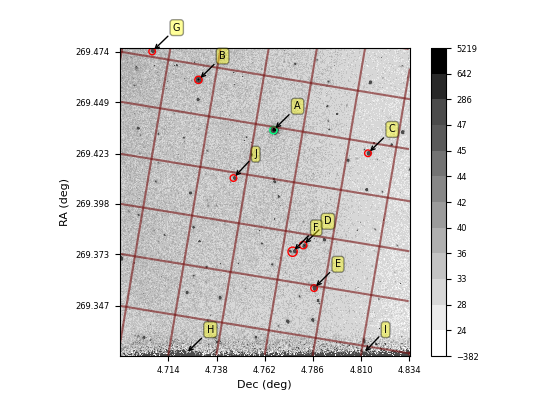
\includegraphics[scale=1]{images/initgexample.png}
\end{center}   
\caption{This is an observation of {\bstar} taken with the \texttt{g} filter on
17 September 2018 at 02:58:52 UTC after processing using the master bias and
flat files for September 2018. The brightest object, marked \textbf{A} and marked in
green is \bstar, whilst the next 9 brightest objects are marked in yellow and
\textbf{B}, \textbf{C}, etc. in decreasing order of brightness.}
\protect\label{fig:initgexample}
\end{figure}

\begin{figure}[!htbp]
\begin{center}
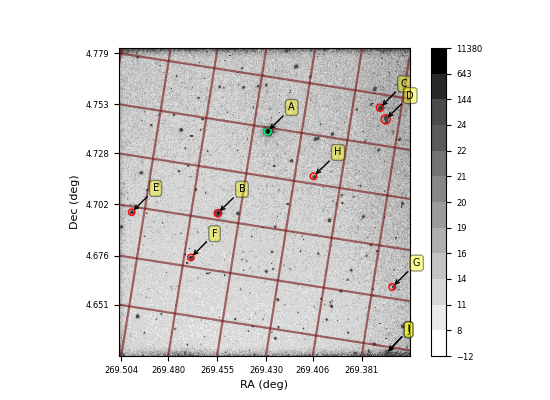
\includegraphics[scale=1]{images/initgexample20.png}
\end{center}   
\caption{This is an observation of {\bstar} taken with the \texttt{g} filter on
7 March 2020 at 09:07:23 UTC after processing using the master bias and
flat files for March 2020. The brightest object, marked \textbf{A} and marked in
green is \bstar, whilst the next 9 brightest objects are marked in yellow and
\textbf{B}, \textbf{C}, etc. in decreasing order of brightness.}
\protect\label{fig:initgexample20}
\end{figure}

In nearly every case there are 4 images taken, one with each of the 4 visible
light filters (in addition to the simultaneous REMIR observations) and in Fig.
\ref{fig:initgexample} is illustrated a set of observations of {\prox} taken on
the same date, 17 September 2018 as the observation of {\bstar} in Fig.
\ref{fig:initgexample}. For comparison, in Fig. \ref{fig:init4example20} is
shown a set of observations taken on 9 March 2020.

\begin{figure}[!htbp]
\begin{center}
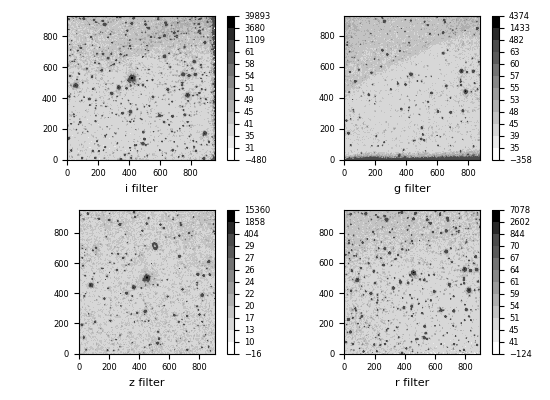
\includegraphics[scale=1]{images/init4example.png}
\end{center}   
\caption{This is all 4 observations of {\prox} taken with the visible light
filters on 17 September 2018 at 02:12:40 UTC after processing using
appropriate master bias and flat files for September 2018. They are arranged in
the order and orientation in which they are taken from the CCD. The
divisions on each image are pixel numbers.}
\protect\label{fig:init4example}
\end{figure}

\begin{figure}[!htbp]
\begin{center}
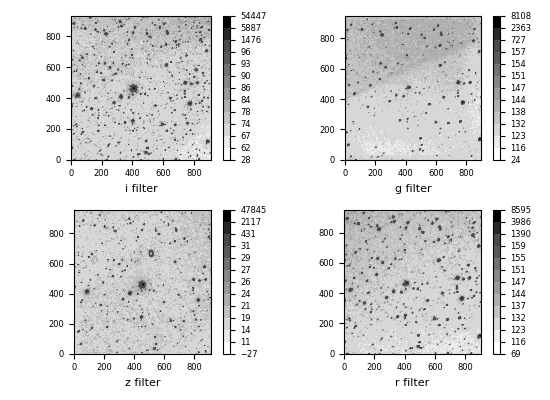
\includegraphics[scale=1]{images/init4example20.png}
\end{center}   
\caption{This is all 4 observations of {\prox} taken with the visible light
filters on 9 March 2020 at 08:56:14 UTC after processing using
appropriate master bias and flat files for March 2020. They are arranged in
the order and orientation in which they are taken from the CCD. The
divisions on each image are pixel numbers.}
\protect\label{fig:init4example20}
\end{figure}

\subsubsection{Some sample light curves}
\protect\label{section:samplelightcurves}

In Fig. \ref{fig:lcurvesing} is presented light curves of ADUs from {\prox}
from the observations on 16 and 17 September 2018 for the \texttt{g} and
\texttt{r} filters. In Fig. \ref{fig:lcurveref} is shown the same observations
where the ADUs are divided by the total ADUs of a subset of objects common to
all of the the other observations.

\begin{figure}[!htbp]
\begin{center}
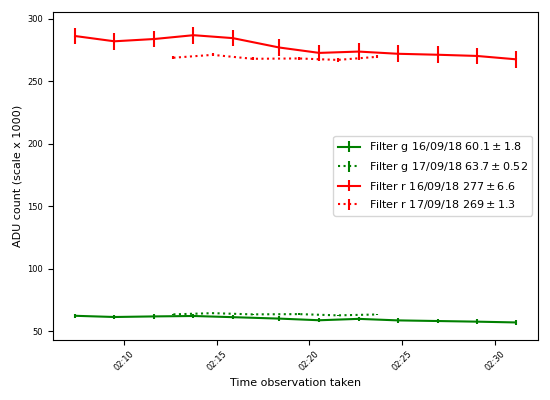
\includegraphics[scale=1]{images/demo_lcurve.png}
\end{center}   
\caption{This shows the total ADUs from the observations of {\prox} on 16 and
17 September 2018 for the \texttt{r} and \texttt{g} filters. The plot for each
day is overlaid to show the time taken.The results for those filters are in the appropriate colours
with the later date dotted.}
\protect\label{fig:lcurvesing}
\end{figure}

\begin{figure}[!htbp]
\begin{center}
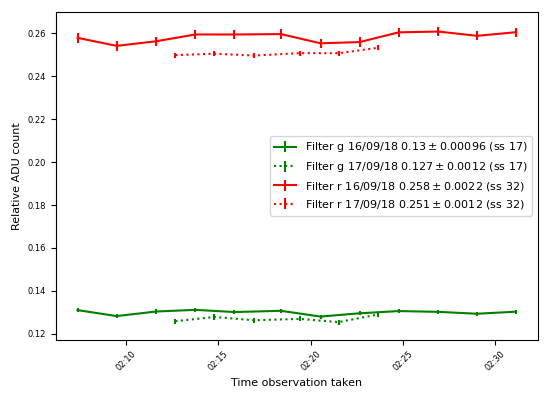
\includegraphics[scale=1]{images/demo_lcurve_refs.png}
\end{center}
\caption{This shows the total ADUs from the observations of {\prox} on 16 and
17 September 2018 for the \texttt{r} and \texttt{g} filters, (the same as in
Fig. \ref{fig:lcurvesing}) divided by the total of the ADUs for a subset of
other objects common to all the observations. The legend in each case shows the
subset size of the reference objects. }
\protect\label{fig:lcurveref}
\end{figure}

\clearpage

% \subsection{Point spread functions}
% \protect\label{section:pointspreadfunc}
% 
% In Fig. \ref{fig:im3d} is shown a 3D representation of the \texttt{g} filter
% observation of {\prox} shown in Fig. \ref{fig:init4example}.
% 
% \textit{I plan to zoom in on some of the objects showing the cross-section in
% various planes to illustrate that the objects are close to Gaussian in profile.
% I then show how I can optimise the aperture for the objects to give an
% acceptable accuracy across various frames. Also note that circular apertures
% are sufficient, sufficiently few would benefit from using an elliptical
% aperture to merit time being spent on these.}
% 
% \begin{figure}[!htbp]
% \begin{center}
% 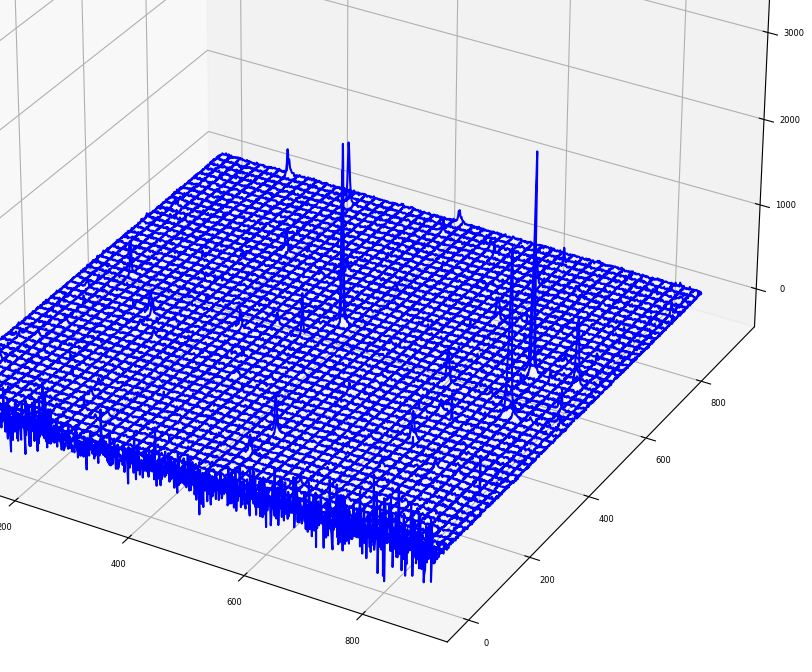
\includegraphics[scale=0.5]{images/im3d.png}
% \end{center}
% \caption{This is a 3-D representation of the \texttt{g} filter observation of
% {\prox} already shown in Fig. \ref{fig:init4example} illustrating the peaks of
% some of the objects.} \protect\label{fig:im3d}
% \end{figure}
% 
% \clearpage

\subsection{Matters addressed in analysing data}
\protect\label{section:mattersaddressed}

The results of the initial processing of the data as discussed above highlighted
the matters which should be addressed to accurately process the images.

\subsubsection{Uncertainty measure}
\protect\label{section:issueuncertainty}

The light curves shown in Fig. \ref{fig:lcurvesing} and Fig. \ref{fig:lcurveref}
have error bars shown according to the standard deviation of the ADU count and
the ratio to the reference stars respectively. Given that the observations are
taken over an initial period of at most 20 minutes, it is unsurprising that
these do not vary much. Part of the variations which are shown may be due to
varying noise in the pixels on the CCD which are different for each exposure.

However the observations are all using the same master flat and bias files. It
is not clear what the uncertainty is on those files, so some analysis is
necessary.

\subsubsection{Flat files}
\protect\label{section:issueflatfiles}

It is of concern that there is a shading towards the bottom of the image; this
is the \texttt{g} filter, for which the bottom part of the image is taken from
the central part of the CCD (the \texttt{g} filter image is taken from the
upper right portion of the CCD, with the origin close to the centre of the CCD).
In Fig. \ref{fig:init4example} is the set of all visible light observations of
\prox, taken on the same date as in Fig. \ref{fig:initgexample} of 17 September 2018 at
02:12:40 UTC, with the images displayed in the sequence in which they are taken
from the CCD. For comparison, the same observations, without application of the
flat fields (but still with subtraction of the bias fields), are presented in
Fig. \ref{fig:init4exnoflat}. Also for comparison, in Fig.
\ref{fig:init4example20}, are observations of {\prox} parallel to those in Fig.
\ref{fig:init4example} from March 2020.

\begin{figure}[!htbp]
\begin{center}
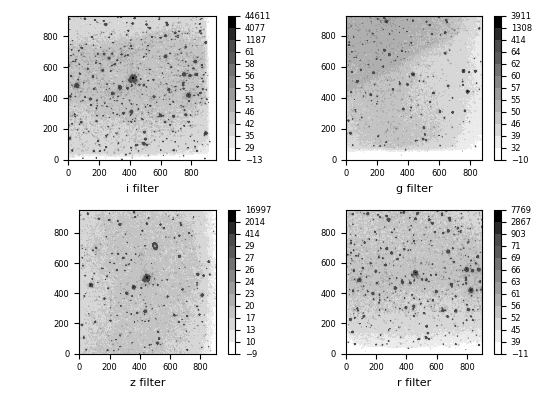
\includegraphics[scale=1]{images/init4exnoflat.png}
\end{center}   
\caption{This is all 4 observations of {\prox} taken with the visible light
filters on 17 September 2018 at 02:12:40 UTC, the same as in Fig.
\ref{fig:init4example}, after processing using appropriate master bias but
omitting the flat files for September 2018. The divisions on each image are pixel numbers.}
\protect\label{fig:init4exnoflat}
\end{figure}

It can be seen that the shading at the sides of the images is introduced by
applying the master flat fields.

\subsubsection{Negative pixels}
\protect\label{section:issuenegpixels}

Of additional concern is that a number of the pixel values are
negative after subtracting the bias value for each pixel. This in some cases is
larger than the pixel value at the same location in the observation file.
It would be expected that the bias level, with exposure of zero, should be
everywhere lower than any pixel observing sky, but this is not the case. For the images shown in Fig.
\ref{fig:init4example} the number of negative pixels are as shown in Table
\ref{table:initexnegpix}.

\begin{table}[!htbp]
\begin{center}
\begin{tabular}{lrrr} \hline
Filter & No of pixels & No negative & \% \\\hline
g & 818,296 & 763 & 0.09 \\
r & 858,600 & 388 & 0.05 \\
i & 898,560 & 2,143 & 0.24 \\
z & 866,136 & 1,401 & 0.16 \\
Total & 3,441,592 & 4,695 & 0.14 \\

\hline
\end{tabular}
\end{center}
\caption{Negative pixels in the images shown in Fig. \ref{fig:init4example} for
the various filters.}.
\protect\label{table:initexnegpix}
\end{table}

\subsubsection{Other caveats}
\protect\label{section:otherissues}

Of some concern is the ring shaped artefact above and slightly to the right of
the brightest objects in the images for the \texttt{z} filter, invariably for
the target, but to a greater or lesser degree for the other objects. Often the
artefact lands entirely on another object, compromising the usability of the
frame.

The \texttt{z} filter is poorest in terms of other objects in the frame for all
of the objects and there are few objects to be found in common subsets across
all the frame, this being because, despite being classified as ``visible
light'', it is in the near Infrared and the {\rdwarf} targets are much brighter
in this band then the other objects.

As a result, it proved advisable to avoid the \texttt{z} filter as it would not
be practical to try to compensate for the artefact given the likely poor return
if this were done. In any case the this is often worst or next to worst in terms
of the number of the negative pixels are to be found in the observations from
this filter, as shown in Table \ref{table:initexnegpix}.

\clearpage

\section{Analysis}
\protect\label{section:tanalysis}

The performance in terms of finding objects, especially with the filters other
than \texttt{g} and \texttt{r} was not good. The various files in use were
considered in turn in an effort to improve the performance.

\subsection{Bias Files}
\protect\label{section:biasfiles}

It was noticeable that some of the pixel values, after subtraction of the master
bias files, became negative, as can be seen in both Fig. \ref{fig:exampmontage}
and \ref{fig:yearapart}. This occurs in a significant number of cases, but
particularly with the \texttt{g} filter, for example example, taking the
observations and master bias files for 5  September 2018, the total negative values shown in 
Table \ref{table:negmast} are
observed.

\begin{table}[!htbp]
\begin{center}
\begin{tabular}{lrr} \hline
Filter & Min & \% negative \\\hline
g & -27 & 28.90 \\
i & -20 & 5.42 \\
r & -19 & 5.52 \\
z & -20 & 9.90 \\
\hline
\end{tabular}
\end{center}
\caption{Negative values of pixels in image minus monthly master bias for
various filters on 5 September 2018, for all observations of \bstar, through
various visible light filters}.
\protect\label{table:negmast}
\end{table}

It is noticeable that this is worst on the \texttt{g} filter, for which some of
the best results were obtained finding images. An example of the distribution of
negative values after subtracting the appropriate master bias from the sky is
shown in Fig.
\ref{fig:negbiaseg}

\begin{figure}[!htbp]
\begin{center}
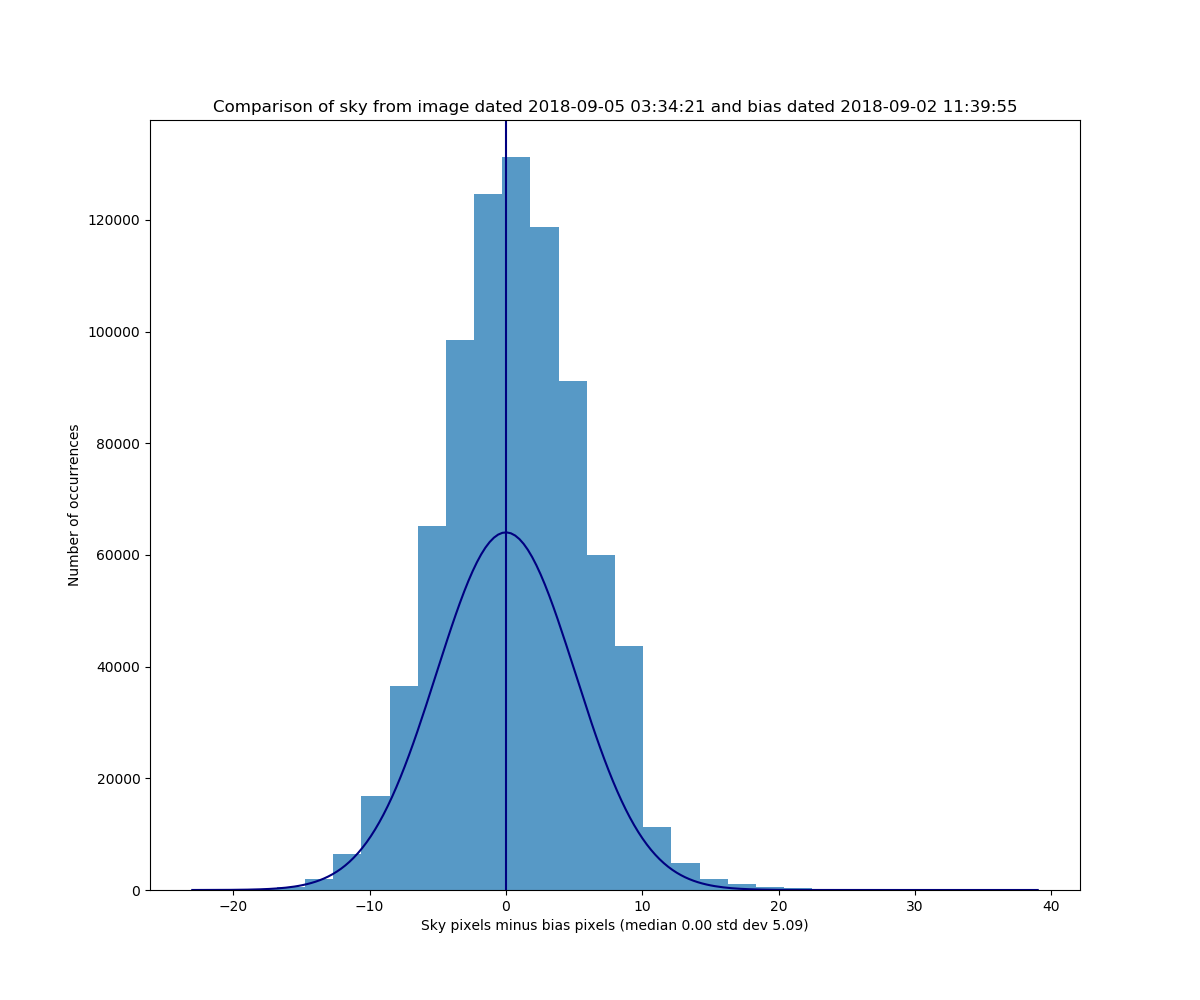
\includegraphics[scale=0.5]{images/negbiaseg.png}
\end{center}   
\caption{This shows the distribution of the values of the sky level pixels minus
the corresponding bias pixels for an observation of {\bstar} with the \texttt{g}
filter taken on on 5 September 2018 and the master bias file for September 2018.}
\protect\label{fig:negbiaseg}
\end{figure}

\subsubsection{Comparison of bias files}

The master bias files are constructed from daily bias files and it seemed
appropriate to examine these. on 5 September 2018, five daily bias files were
taken between 11:31:10 UTC and 11:37:02 UTC for each filter.

Each consecutive pair of bias files were compared against each other (after
eliminating ``spikes'') and the results set out in Fig.
\ref{fig:biascomp}.

\begin{figure}[!htbp]
\begin{center}
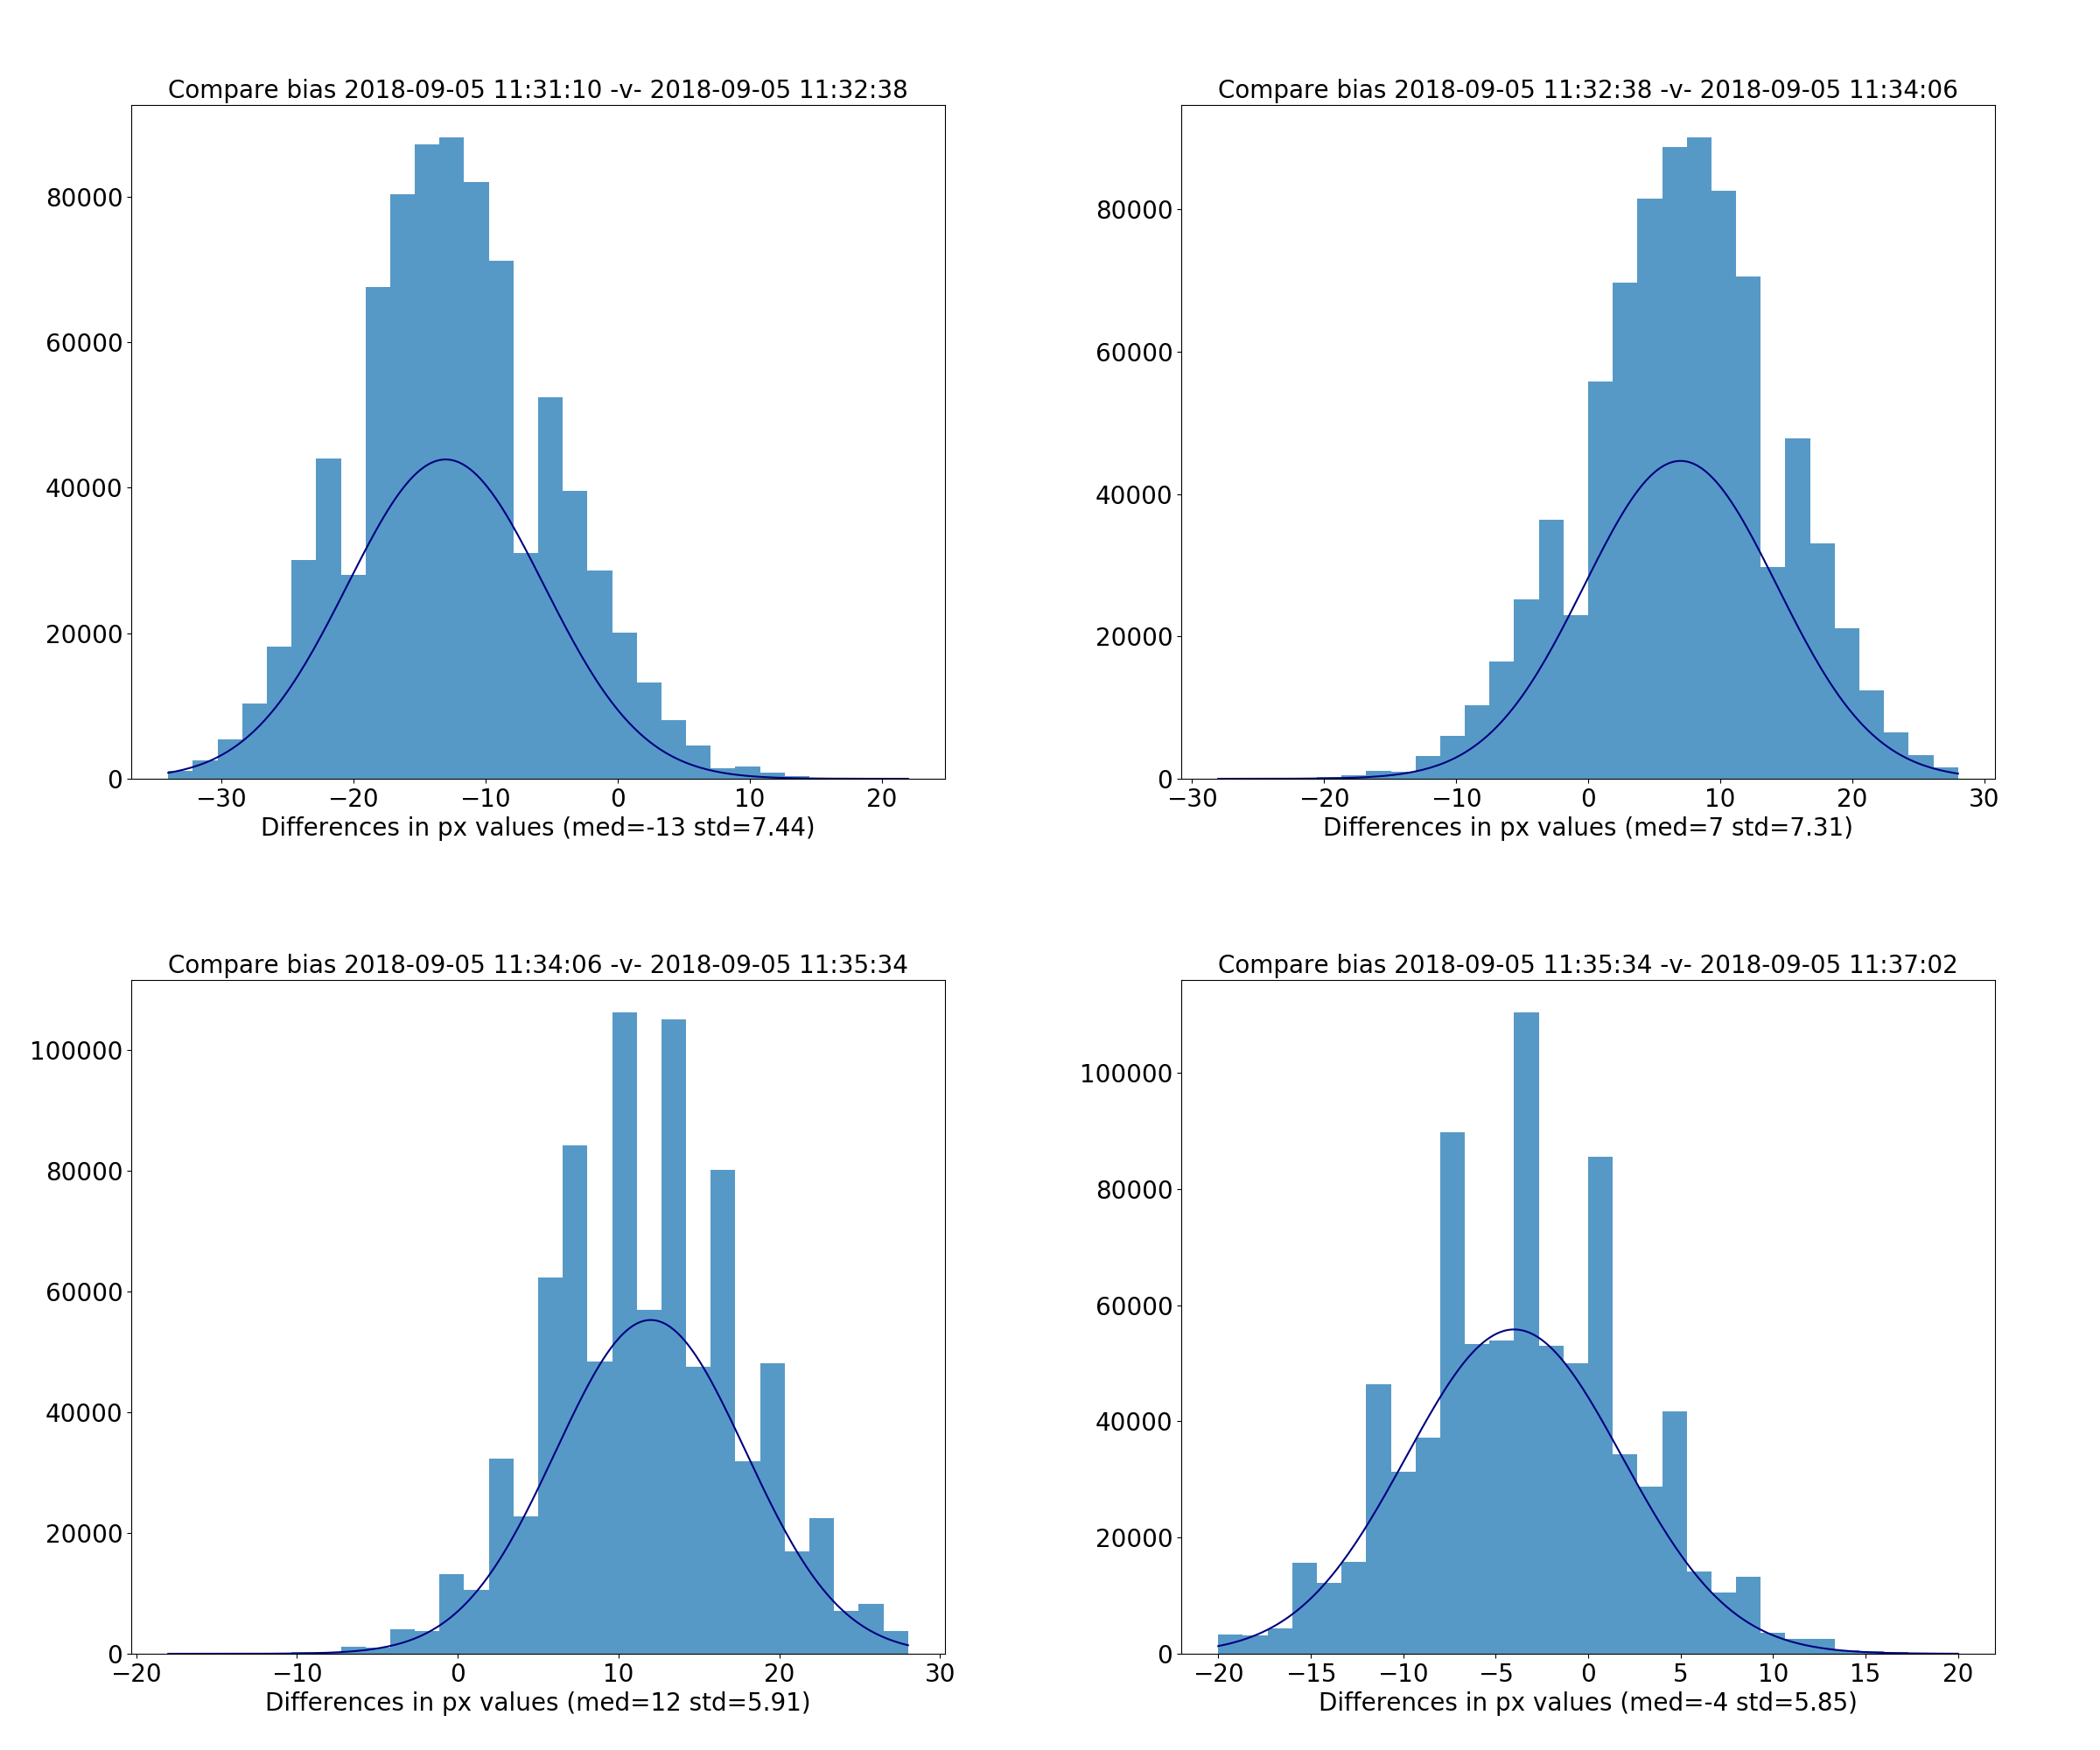
\includegraphics[scale=0.2]{images/biascomp.png}
\end{center}   
\caption{This shows the differences between successive pairs of the 5 bias
files taken on 5 September for filter \texttt{g} with times as shown in the
titles between 11:31:10 UTC and 11:37:02 UTC} \protect\label{fig:biascomp}
\end{figure}

Similar results were observed when bias files for other filters were observed,
for other dates and daily bias files several days apart were compared. The
differences would appear to be a measure of the errors in the CCD used.

A bias file was constructed by merging together all the daily bias files and the
computation shown in Fig. \ref{fig:negbiaseg} for the monthly master
bias file repeated, the result is very similar, as shown in Fig.
\ref{fig:negbiasmerg}.

\begin{figure}[!htbp]
\begin{center}
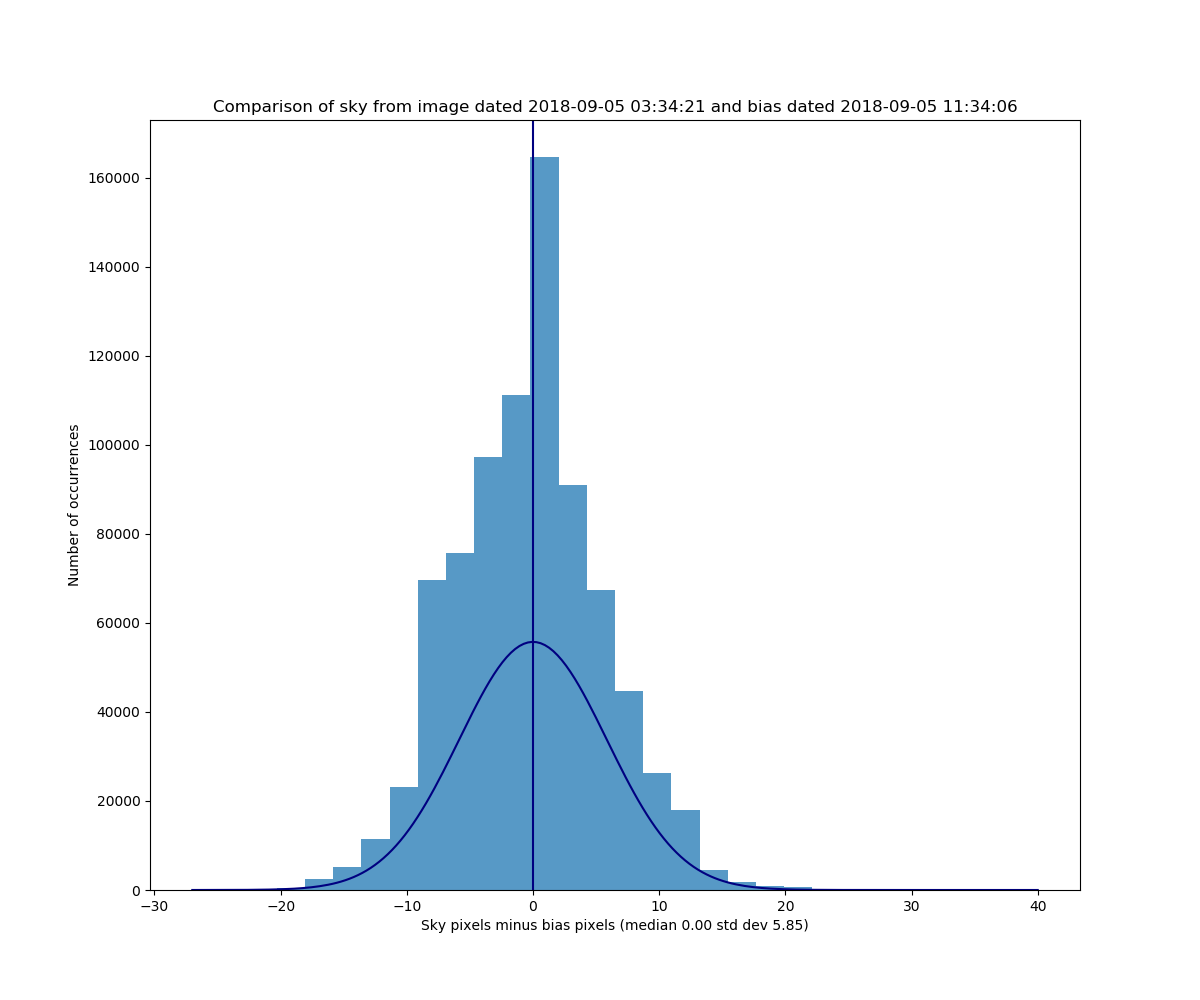
\includegraphics[scale=0.5]{images/negbiasmerg.png}
\end{center}   
\caption{This shows the distribution of the values of the sky level pixels minus
the corresponding bias pixels for an observation of {\bstar} with the \texttt{g}
filter taken on on 5 September 2018 and a bias file constructed from the bias
files taken on 5 September 2018.} \protect\label{fig:negbiasmerg}
\end{figure}

It was noticeable that, except in the case of images which were clearly
defective in other ways, the difference between the merged bias levels and the
sky levels was at most that of the standard deviation between the bias levels
shown in Fig. \ref{fig:biascomp} and was often zero as Fig.
\ref{fig:negbiaseg} and Fig. \ref{fig:negbiasmerg} show. This would suggest that
the bulk of the ``sky level'' is made up of the bias values.

\subsubsection{Hotspots or defective pixels}
\protect\label{section:hotspots}

It was noticeable that apparent findings of objects in the images consistently
showed a point source. This was particularly true of the images for the
\texttt{g} filter. It was attempted to identify such hotspots by examining the
number of bias file images in which a peak value of over 5 standard deviations appears in the same place in over 1\% of the files,
it was found that there were 1,558 such pixels in all the
\texttt{g} daily bias files, 2 in the \texttt{z} files and none in the others.
793 were in column 623, where the vertical line appears in the images and can be
seen in Fig. \ref{fig:yearapart}. No amount of adjustments to flat or bias files
can be made to overcome this consistently. It will have to be worked around by
interpolation over the areas in question.

It is unfortunate that this applies to the \texttt{g} filter as the images are
otherwise better than the others. Possibly this might give rise to ``false
positives''.

\subsubsection{Master bias files}
\protect\label{section:masterbias}

The master bias files are created by combining all the bias files for the
relevant month, using the median pixel value in each case. This is reasonable
in most cases except for the \texttt{g} filter case where there are so many
hotspots. This probably explains the high number of negative pixels after
applying the bias files noted in Table \ref{table:negmast}.


\subsection{Flat files}
\protect\label{section:flatfiles}

Two kinds of flat file are provided, a set of daily flat files for each of the
filters, typically 2 or 3 each day for each of the 4 visible light filters \textbf{g},
\textbf{i}, \textbf{r} and \textbf{z} and for gains of 1 and 4 and the monthly
master flat files, consisting of a composite of the daily flat files for the
month.

\subsubsection{Daily flat files}
\protect\label{section:dailyflatfiles}

The daily flat files, after the end of 2013, which precedes the first of the
observations, are taken with an exposure time of 1 second. Some have a gain of
4.4, in line with the gain applied to some of the other observations, but in
this report only the flat files with a gain of 1 are considered. The master flat
files are only taken from these.

Rows and columns of the image containing zero pixels were removed from the
images before analysis. (These values are replaced by \texttt{NaN} in cle master
flat files and correspond to invalid pixels.)

It was of concern that many of the daily flat files had pixels which were vary
close to saturation. in some cases they were clearly saturated, but none of the
master flat files appeared to incorporate the daily flat files with definitely
saturated pixels. In Table \ref{table:satpix} is shown the proportion of
nearly saturated pixels in flat files for each filter.

\begin{table}[!htbp]
\begin{center}
\begin{tabular}{lrrr} \hline
Filter & Flat files & Saturated & Over 50\%\\\hline
g & 3,679 & 29.49 & 22.34 \\
i & 3,679 & 32.37 & 27.43 \\
r & 3,680 & 32.66 & 28.12 \\
z & 3,680 & 0.92 & 0.60 \\\hline
Overall & 14,718 & 23.86 & 19.62\\
\hline
\end{tabular}
\end{center}
\caption{Breakdown of daily flat files by filter up to August 2019 showing
number, percentage with nearly saturated pixels present and percentage with over
50\% saturated pixels (in many cases this was over 90\% and occasionally 100\%).}
\protect\label{table:satpix}
\end{table}

\subsubsection{Linearity of CCDs}

It might be reasonable to expect that if the CCDs are linear, then the standard
deviation of the values in the daily flat files would rise in proportion to the
mean values in the daily flat files. In Fig. \ref{fig:ffcorr} is shown how this
correlates for the four filters.

\begin{figure}[!htbp]
\begin{center}
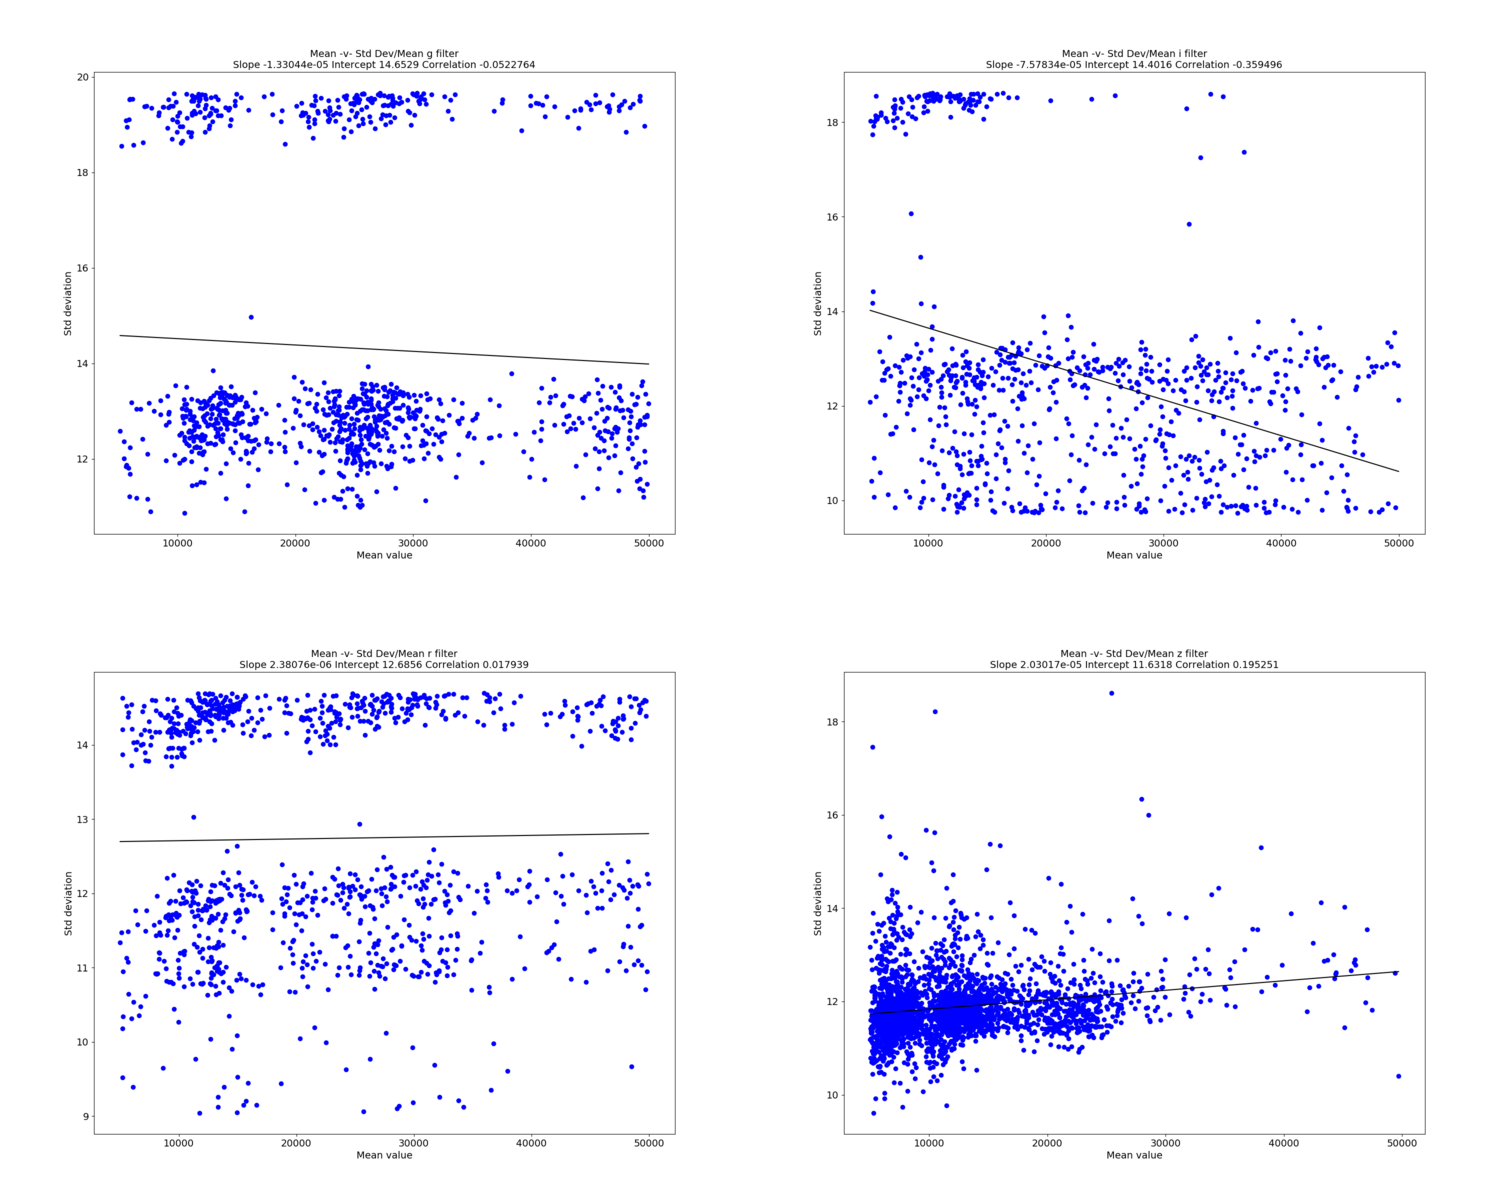
\includegraphics[scale=0.25]{images/Corr.png} \\
\end{center}   
\caption{This figure shows how the standard deviation of the values in the
daily flat files corresponds to the four filters. In the top is shown the
results for the \texttt{g} filter, the bottom left shows the \texttt{r} filter,
the top right shows the results for the \texttt{i} filter and the bottom right
shows the results for the \texttt{z} filter. The black line shows the best fit
slope in each case.}
\protect\label{fig:ffcorr}
\end{figure}

It is clear \textit{and I need another diagram to illustrate this} that
linearity drops off dramatically when the mean is below 5,000 and above 50,000.
%\
\subsubsection{Master flat files}
\protect\label{section:masterflatfiles}

The master flat files consist of median values of the incorporated daily flat
files, the header indicating which ones are considered.

Invalid pixel values are represented by \texttt{Nan} and rows and columns
containing these values are trimmed from the images, both for the flat files
themselves, and also for the corresponding bias and observations files.

The program used to create the master flat files selects daily flat files with a
mean value between 5,000 and 50,000 \textbf{and} with a negative skew and
kurtosis less than 7.\footnote{In the author's opinion the ``and'' was not
intended,}

It would appear to the author that the upper limit is too great and several
files with saturated pixels are included, using the median pixel value will
exclude these, but this creates a difficulty in that as 3 daily flat files are
taken from the sky before observations start, effectively the middle one is
taken in each case by the median.

In the author's opinion each flat file should
be normalised first and the results combined, so a procedure to create
alternative master flat files was devised. This turned out to be compromised by
the extreme values in the bias files, which made some of the pixel values
negative in the daily flat files. This primarily affected the \texttt{r} filter
(not the \texttt{g} filter as might have been expected). To complete this task
the hotspots need to be eliminated.

It was noticed that there was a computational error in the calculation of the
mean, standard deviation and other parameters in the master flat files and these
had to be discarded in any event. As the daily flat files change somewhat over
time \textit{I need to illustrate this}, reliance on a master flat file possibly
30 days removed from the observations to which it relates would seem
inappropriate and a procedure of ``rolling'' master flat files centred on the
observation dated was adopted.

\subsubsection{Accuracy}
Combination of daily bias values appears to improve the accuracy. The median
pixel value for all of the bias files for all of the filters is approximately
300 with a standard deviation of about 7 for the individual files, 3 for where
all the daily ones for a given day are merged and 1 for the master bias files.

If the counts on the actual images are considered, the following maximum pixel
values are observed, as illustrated in Table \ref{table:pmaxima}. Note that
these are extreme cases. The typical maximum is about 75\% of these.

\begin{table}[!htbp]
\begin{center}
\begin{tabular}{lr} \hline
Filter & Max pixel value \\\hline
g & 5,010 \\
i & 56,509 \\
r & 16,562 \\
z & 34,293 \\
\hline
\end{tabular}
\end{center}
\caption{Maximum pixel values in any of the observation files for 5 September
2018.}.
\protect\label{table:pmaxima}
\end{table}
\clearpage

% \subsection{Analysis of images}
% \protect\label{section:analimages}
% 
% \textbf{Please note that since I realised that the master flat files are not
% normalised as Luciano told me I'll have to redo all this. The results within
% each month are consistent but not with other months. Also with the flat files
% properly normalised some of the images will have greater contrast.}
% 
% \subsubsection{Intensity comparison}
% \protect\label{section:intcomp}
% 
% As a first attempt to study the data, the ADU count was taken, specifically the
% net after applying the flat and bias files of the target in all the images in which it was available.
% The target was found in all of the images, apart from in a few of the
% \textbf{g}, \textbf{i} and \textbf{r} visible light filters,
%, as shown in Table
%\ref{table:occtb} below.

%Plotting light curves of the intensities obtained in this way yields Fig.
% \ref{fig:allall}.
%Binning the intensities together into a single day gave
%Fig. \ref{fig:allbin}, the error bars indicate the spread over a single day.

%I plotted
%periodograms, as shown in Fig. \ref{fig:pgrams}. Despite the crudeness of the
%data, it is noticeable that there are peaks close to the rotation periods of
% the order of 150 days referred to in \citet{suarezmascareno15} and \citet{toledopadron18}.

% \begin{figure}[!htbp]
% \begin{center}
% 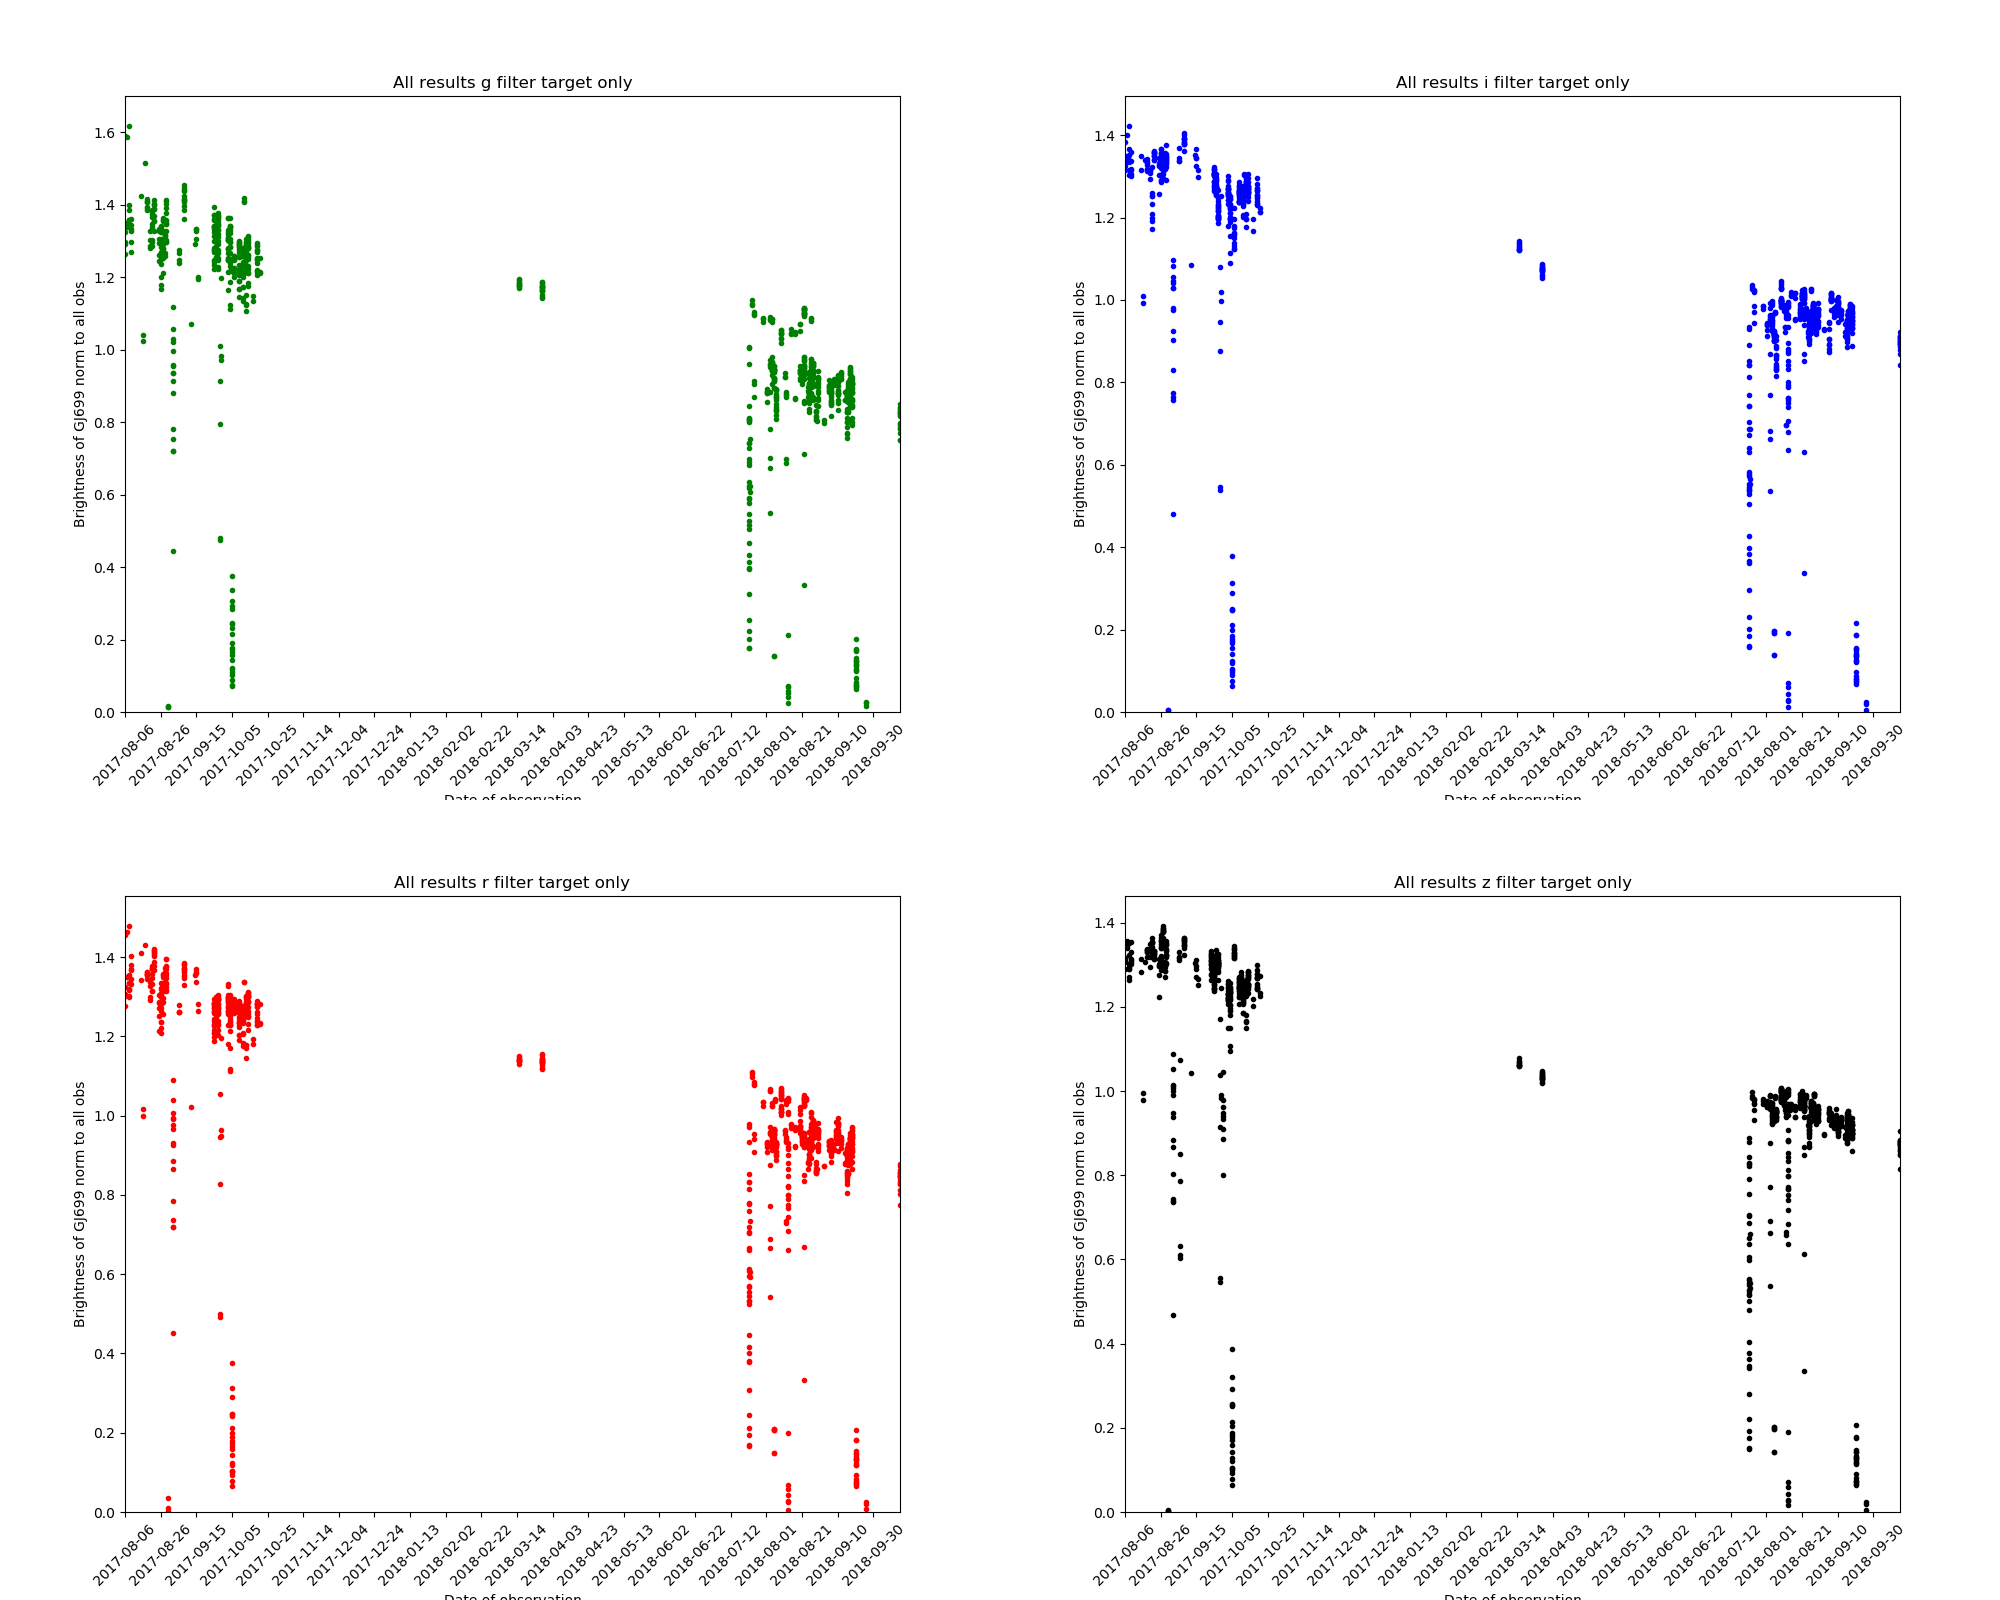
\includegraphics[scale=0.25]{images/allall.png} \\
% \end{center}   
% \caption{This shows the flux for the target, \bstar, for each of the four visible light filters. This takes the total
%   ADU count only}
%   \protect\label{fig:allall}
% \end{figure}
% 
% \begin{figure}[!htbp]
% \begin{center}
% 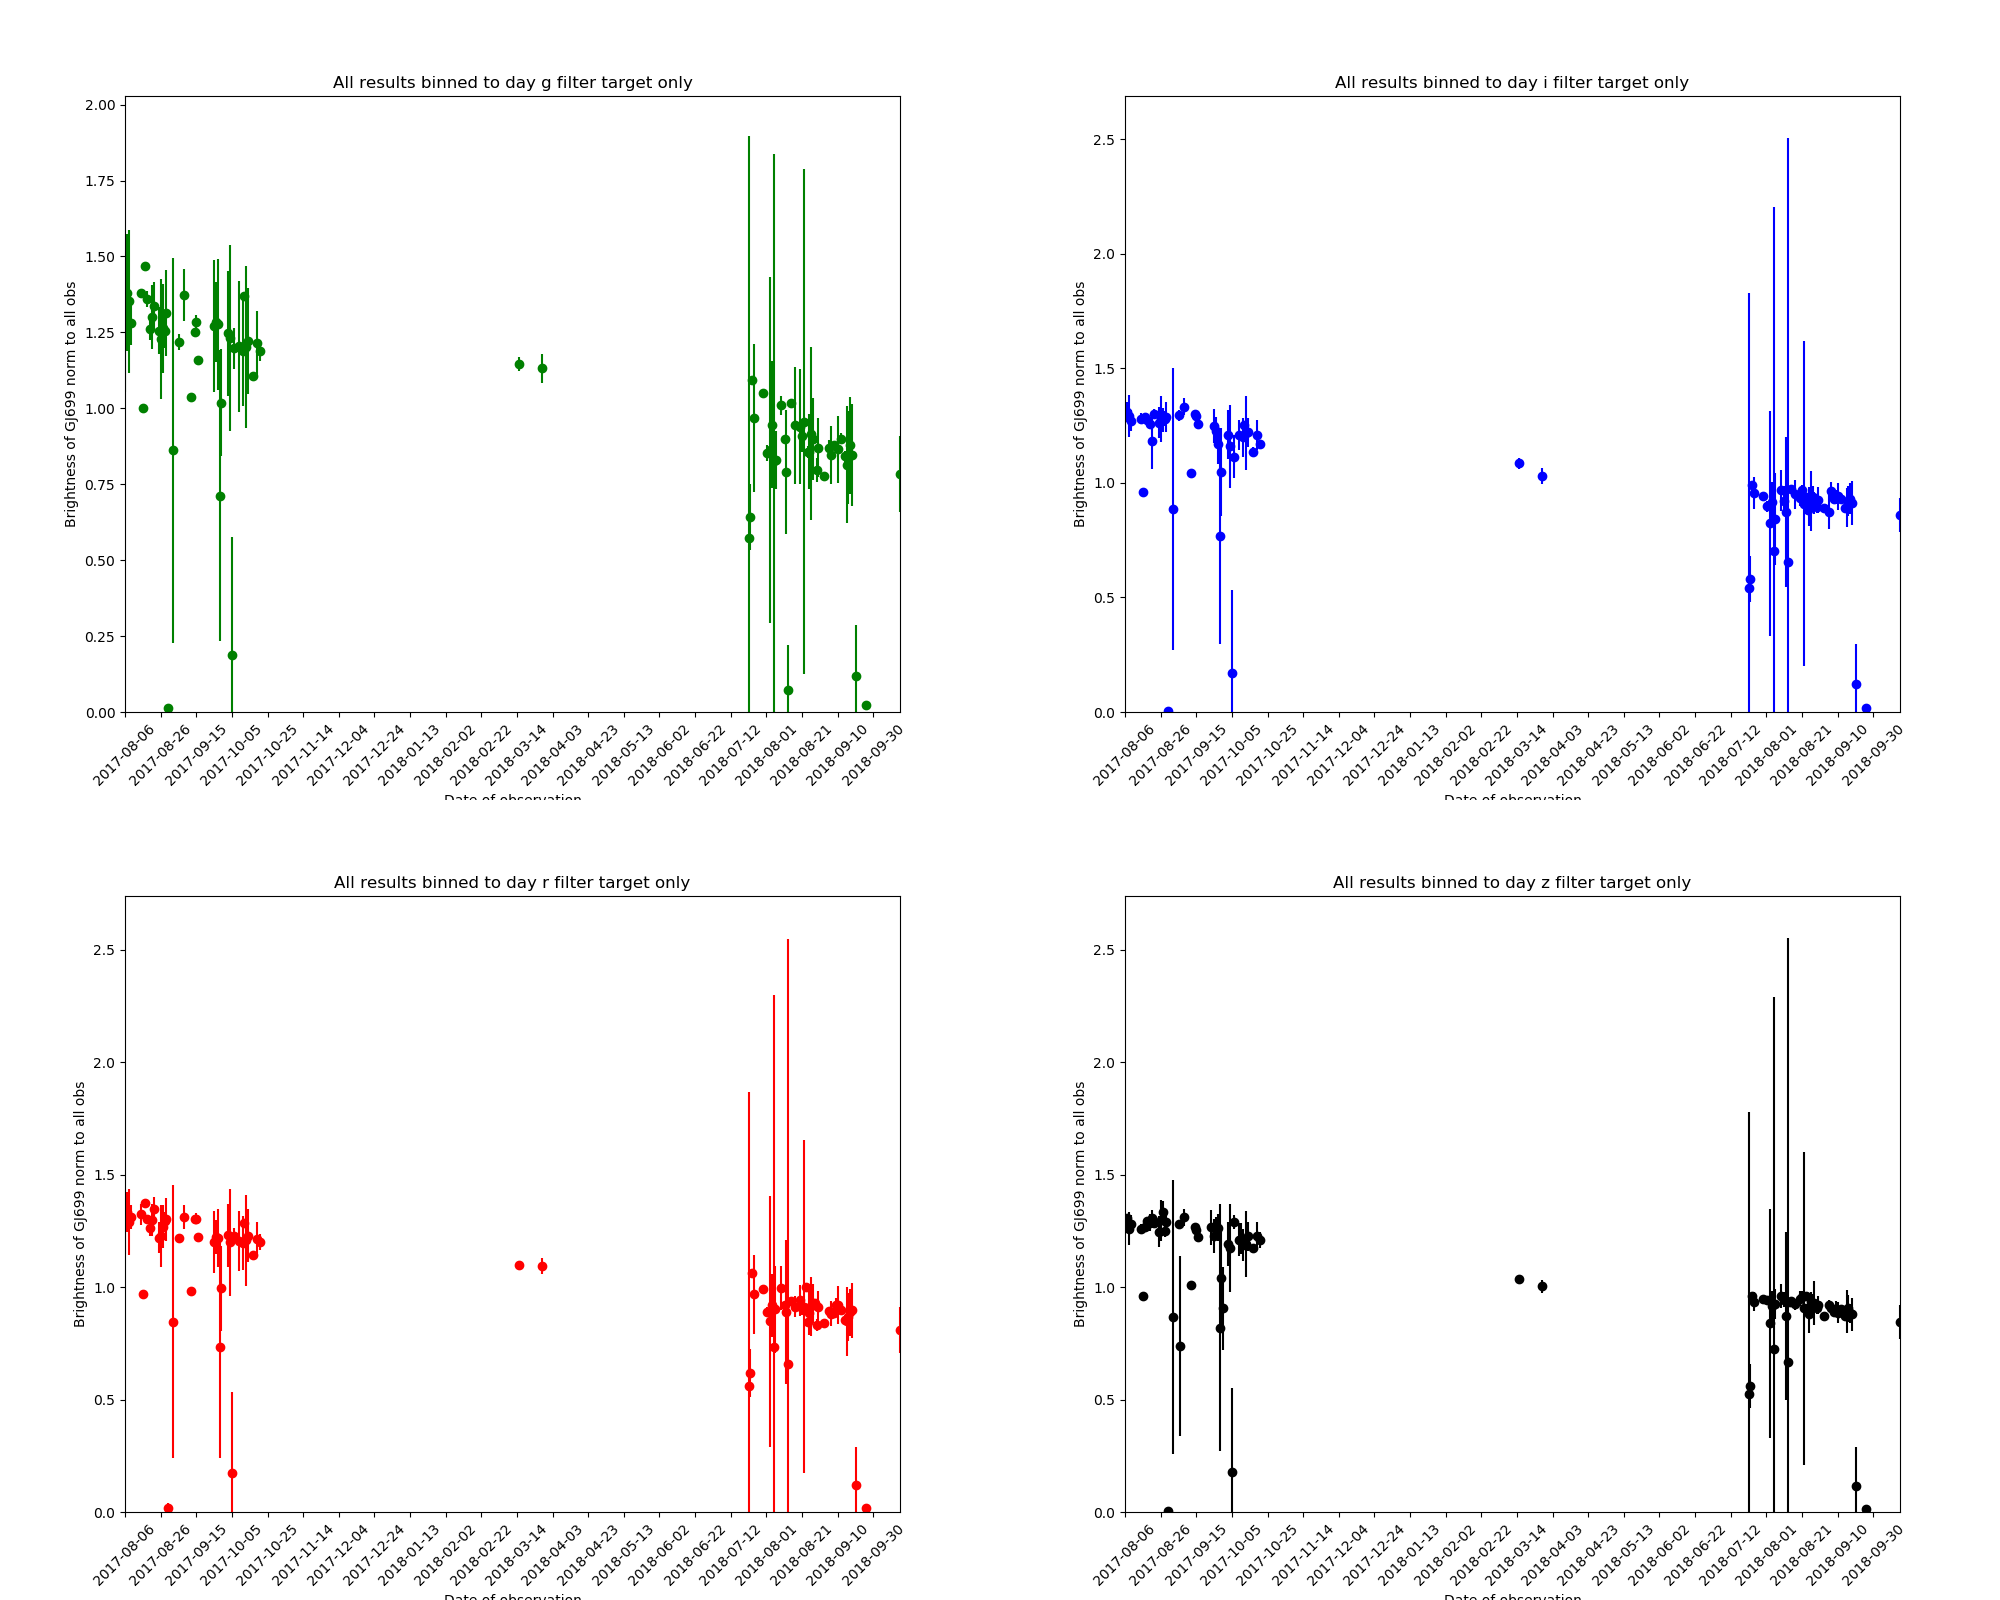
\includegraphics[scale=0.25]{images/allbin.png} \\
% \end{center}   
% \caption{This shows the flux for the target, \bstar, for each of the four visible light filters and binned to a single day. Error bars are show to indicate the spread of intensities over a single day.}
%   \protect\label{fig:allbin}
% \end{figure}

%\begin{figure}[!htbp]
%\begin{center}
%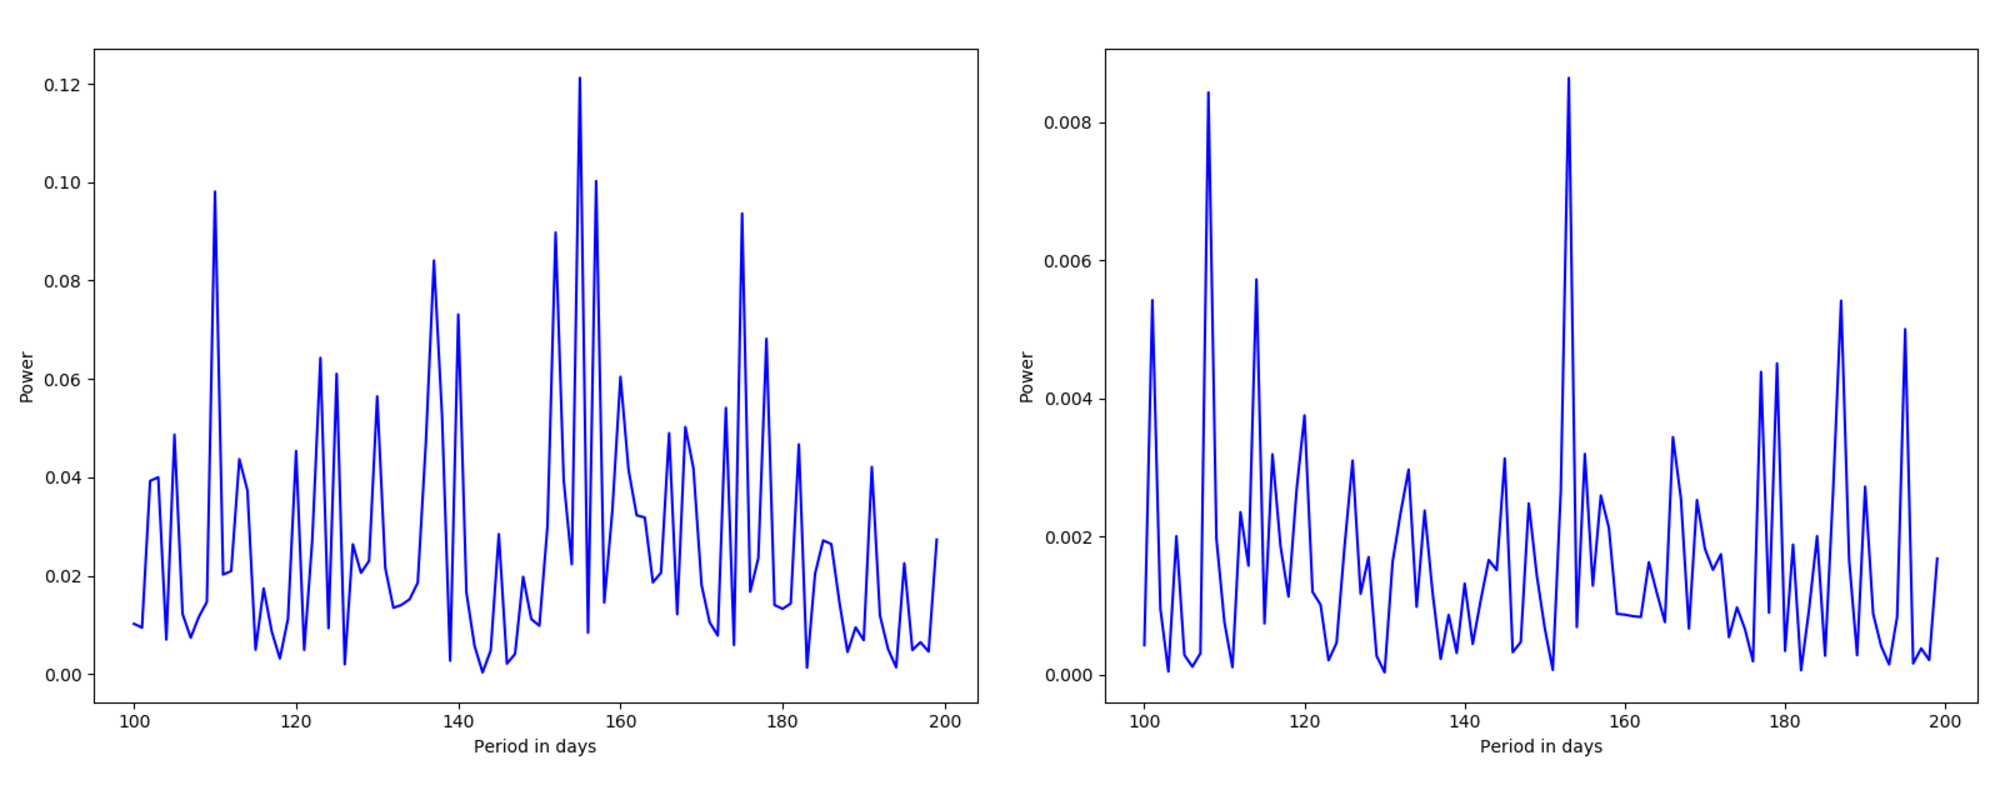
\includegraphics[scale=0.25]{images/pgrambunb.png} \\
%\end{center}   
%\caption{This displays periodograms derived from the binned (Fig.
% \ref{fig:allbin}) and unbinned (Fig. \ref{fig:allall}) light curves for the \textbf{r} filter.}
%  \protect\label{fig:pgrams}
%\end{figure}

% It is accepted that this initial treatment is crude. Serious work needs to be done on correction for air mass,
% which for a few observations, where they are spread over a period of several hours,
% can be quite large, and to more accurately discard as unacceptable images with large or very variable sky levels.
% There are some currently inexplicable variations, for
% example the to images in Fig. \ref{fig:tyeg} give radically different ADU counts despite being taken two minutes apart
% with same exposure time and other parameters.
% 
% \begin{figure}[!htbp]
% \begin{center}
% 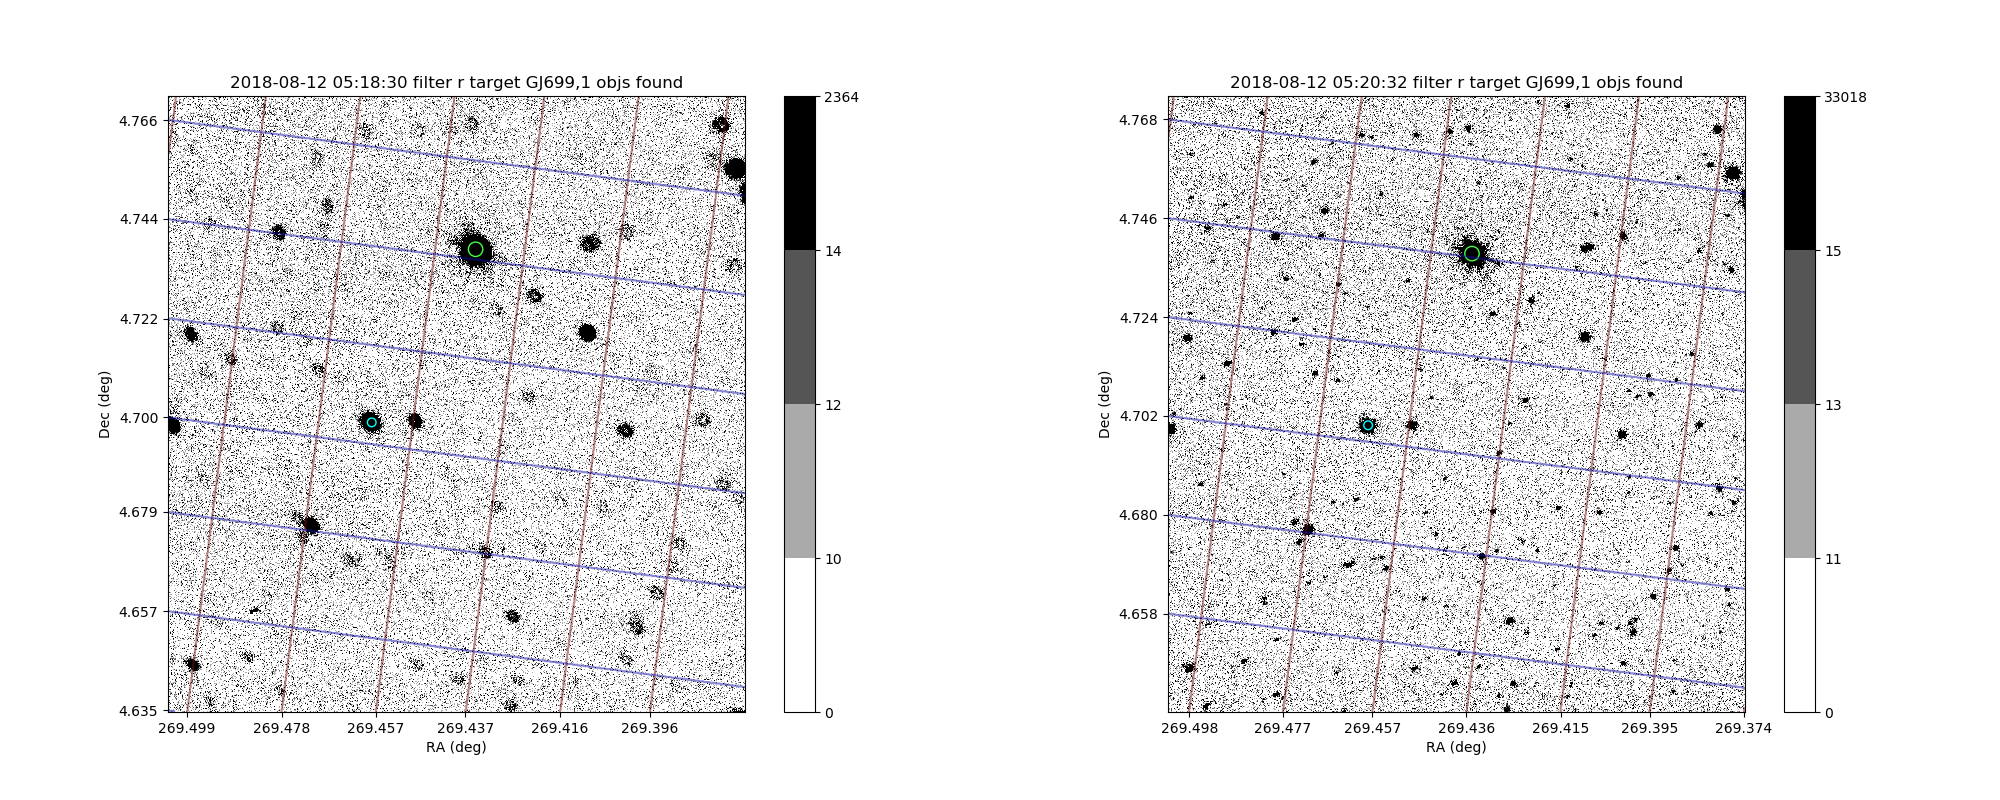
\includegraphics[scale=0.25]{images/tyeg.png}
% \end{center}   
% \caption{These images show an example of where 2 images taken 2 minutes apart with the same exposure time gave different flux values.}
%   \protect\label{fig:tyeg}
% \end{figure}
% 
% \subsubsection{Reference Stars}
% \protect\label{section:refstars}
% 
% Rather than relying on the ``raw'' flux from the target star itself, it was
% considered that an approach based on identified reference stars found in a
% significant number of images.
% Ideally these should be as many as possible to ``smooth'' out errors and variations on the reference star. 
% Byy taking the ratio of the target star ADU count to the sum of the reference
% star ADUs, then we can hope to achieve results for intensity with the factors such air mass corrections factored out, This
% approach was taken in \citet{berry11} and would seem to involve least work, provided sufficient reference stars are
% consistently found.
% 
% The algoritm used to find objects was first to locate the target (there was
% usually a certain amount of error in the coordinates of the images) and then
% find prefeviously-known reference objects. The criterion for finding objects was to look for groups of pixels within a
% given scan aperture whose mean count was a given number of standard deviations
% (intially 3) from that of the sky level. If the result appeared to be one of
% the objects known already, the given reference object was deemed to have been
% found.

% In all cases the brightest objects were found in Simbad, 2MASS and SDSS
% to find objects in the vicinity of \bstar, obtaining the following stars as shown in Table \ref{table:reftimesfound}.
% Of the stars there, the types are unavailable apart from the most-frequently occurring one of
% TYC425-262-1, which is an A3V star (this is also reported as the most frequently found reference star in \citet{berry11}).
% 
% \begin{table}[!htbp]
% \begin{center}
% \begin{tabular}{llr} \hline
% Number & Object & Times found \\\hline
% 1 & TYC425-262-1 & 5,277 \\
% 2 & SDSS1237671695527248969 & 3,408 \\
% 3 & 2MASSJ17574653+0447466 & 3,297 \\
% 4 & SDSS1237668573088841773 & 840 \\
% 5 & TYC425-223-1 & 369 \\
% 6 & SDSS1237671695527249415 & 15 \\
% \hline
% \end{tabular}
% \end{center}
% \caption{This lists the identified reference objects near to {\bstar} and the number of times found in the available
%   data. Note that this data relates to images up to the end of October 2018.}
% \protect\label{table:reftimesfound}
% \end{table}
% 
% I decided to consider only the first 3 reference objects, which are labelled 1, 2 and 3 for convenience in the
% remainder of this report, as the appearances of the others were too infrequent to render them worthwhile.
% 
% \subsection{Classification of results}
% \protect\label{section:classresults}
% 
% The images presented challenges in various respects. The visible light images are all at different orientations and with
% the target in different places in the image, so not all the reference stars appear in all of the images. In some cases
% the reference stars are just not bright enough to rise sufficiently above the sky level.
% 
% \begin{table}[!htbp]
% \begin{center}
% \begin{tabular}{lrrrr}
% &Filter g&Filter i&Filter r&Filter z\\\hline
% Target not found&167&80&105&0\\
% No ref objs found & 84 & 1,003 & 53 & 1,085 \\\hline
% Obj 1 (with or without others) & 834 & 0 & 925 & 0 \\
% Obj 2 (with or without others) & 561 & 1 & 574 & 0 \\
% Obj 3 (with or without others& 526 & 0 & 573 & 0 \\
% Obj 1 only & 43 & 0 & 100 & 0 \\
% Obj 2 only & 0 & 1 & 1 & 0 \\
% Obj 3 only & 0 & 0 & 0 & 0 \\
% Objs 1 and 2 (with or without 3) & 561 & 0 & 573 & 0 \\
% Objs 1 and 3 (with or without 2) & 526 & 0 & 573 & 0 \\
% Objs 2 and 3 (with or without 1) & 296 & 0 & 321 & 0 \\
% Objs 1 and 2 only & 265 & 0 & 252 & 0 \\
% Objs 1 and 3 only & 230 & 0 & 252 & 0 \\
% Objs 2 and 3 only & 0 & 0 & 0 & 0 \\
% Objs 1,2 and 3 & 296 & 0 & 321 & 0 \\
% \hline
% \end{tabular}
% \end{center}
% \caption{This table shows the occurrences of the 3 main reference objects in each of the observations with or without
%   the others. The infrared images were omitted as no reference objects were found in any of them. Note however the lack
%   of occurrences of reference objects in the \textbf{i} and \textbf{z} filter images.}
% \protect\label{table:occtb}
% \end{table}
% 
% \subsection{Results from reference object comparisons}
% \protect\label{section:refobjres}
% 
% Repeating the light curve plots from Section \ref{section:intcomp}, this time as the ratio of the ADU count of the
% target to the sum of the first three reference objects, Fig.  \ref{fig:allref123} and Fig. \ref{fig:allref123bin} show
% the light curves for the \textbf{r} and \textbf{g} filters. Also shown in Fig. \ref{fig:ls123both} are periodograms
% derived from these light curves. Also shown in Fig \ref{fig:allref1}, Fig. \ref{fig:allref1bin} and Fig. \ref{fig:ls1both}
% are the corresponding results taking into account only the brightest of the reference objects, TYC425-262-1.
% 
% \begin{figure}[!htbp]
% \begin{center}
% 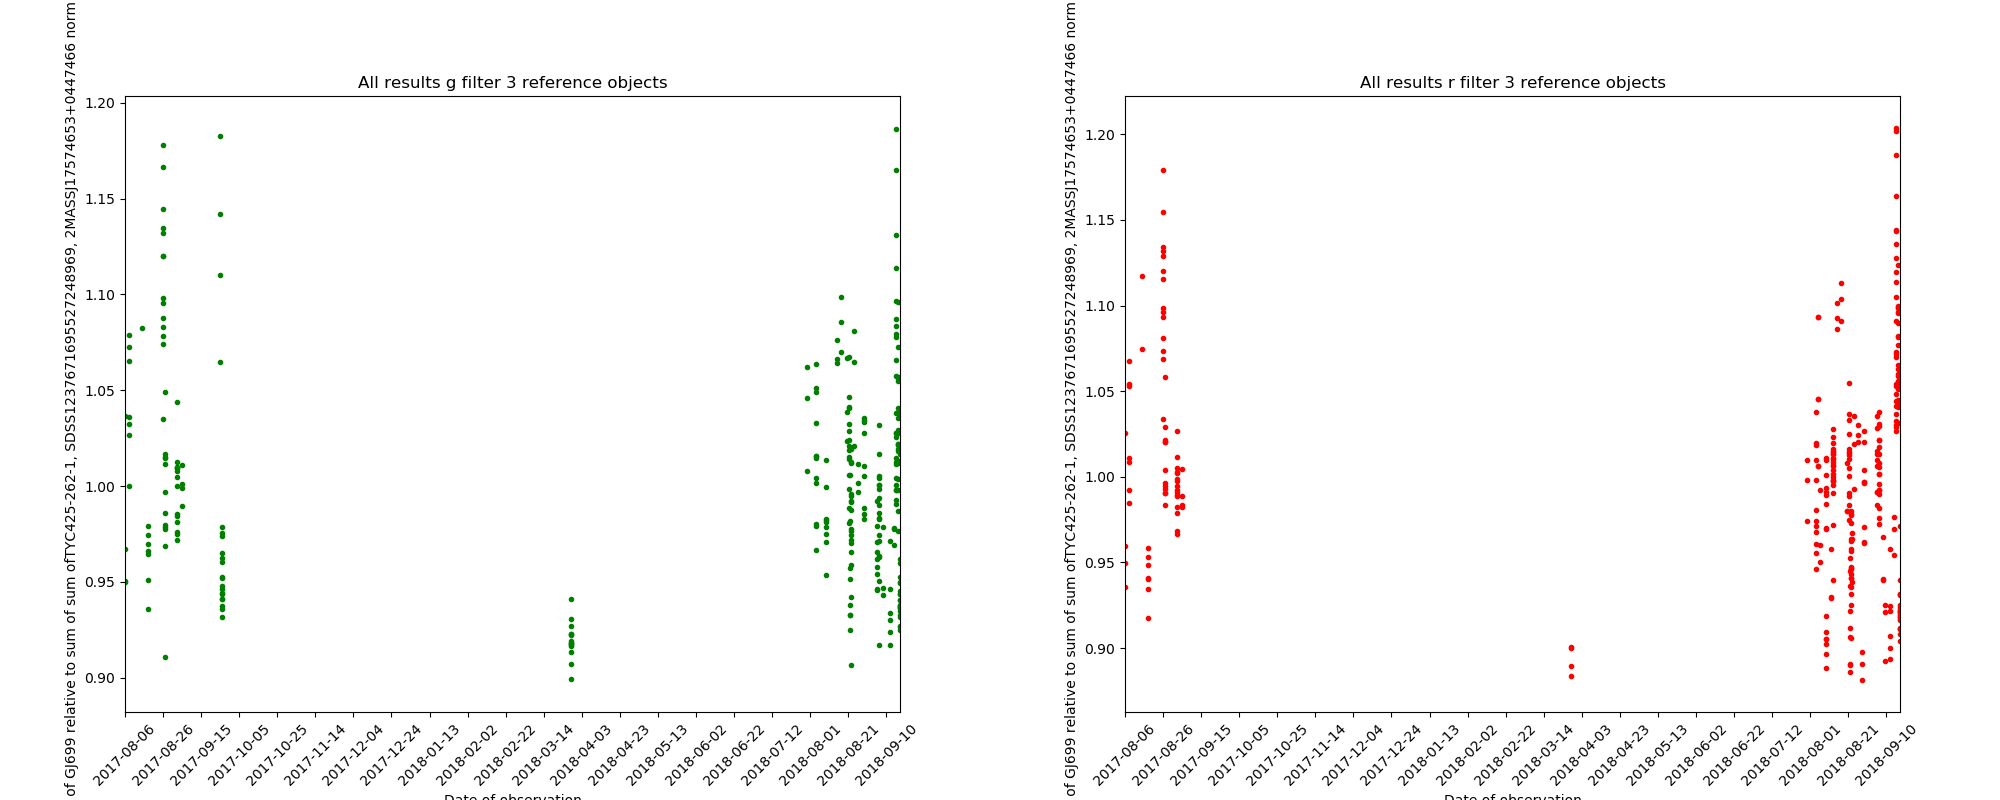
\includegraphics[scale=0.25]{images/allref123.png}
% \end{center}   
% \caption{This shows the ratio of the flux for the target, \bstar, to the 3 main reference objects for the \textbf{g} and
% \textbf{r} filters, plotted as green and red respectively.}
%   \protect\label{fig:allref123}
% \end{figure}
% 
% \begin{figure}[!htbp]
% \begin{center}
% 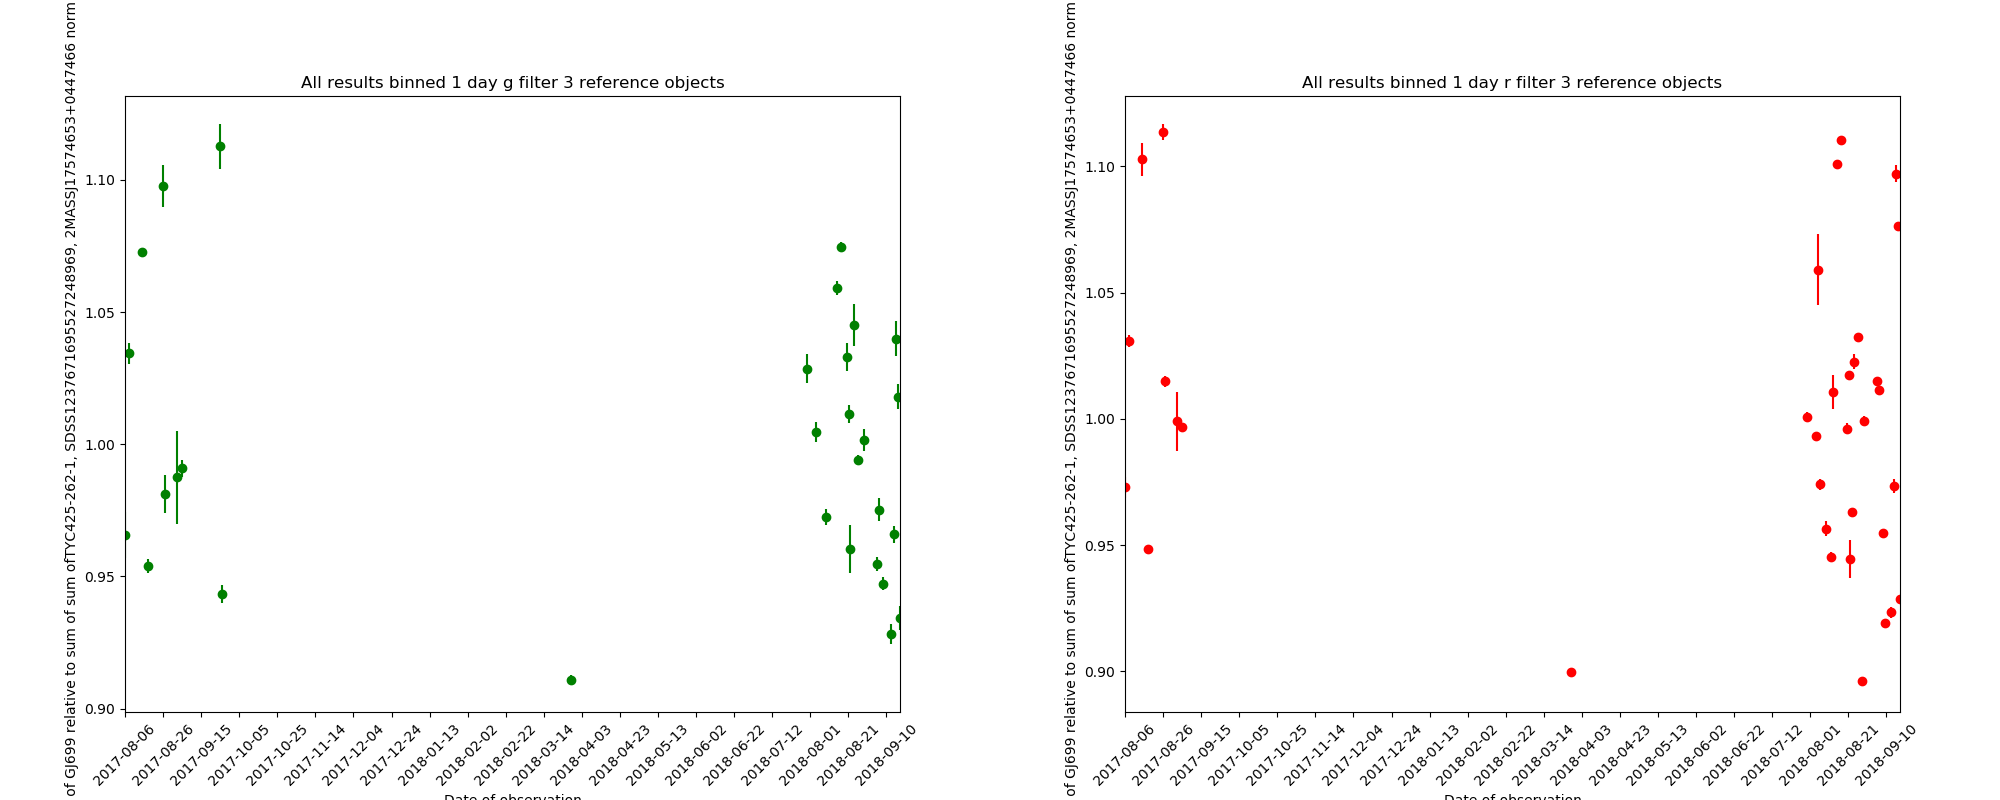
\includegraphics[scale=0.25]{images/allref123bin.png}
% \end{center}   
% \caption{This shows the ratio of the flux for the target, \bstar, to the 3 main reference objects as per Fig. \ref{fig:allref123} and binned to 1 day.}
%   \protect\label{fig:allref123bin}
% \end{figure}
% 
% \begin{figure}[!htbp]
% \begin{center}
% 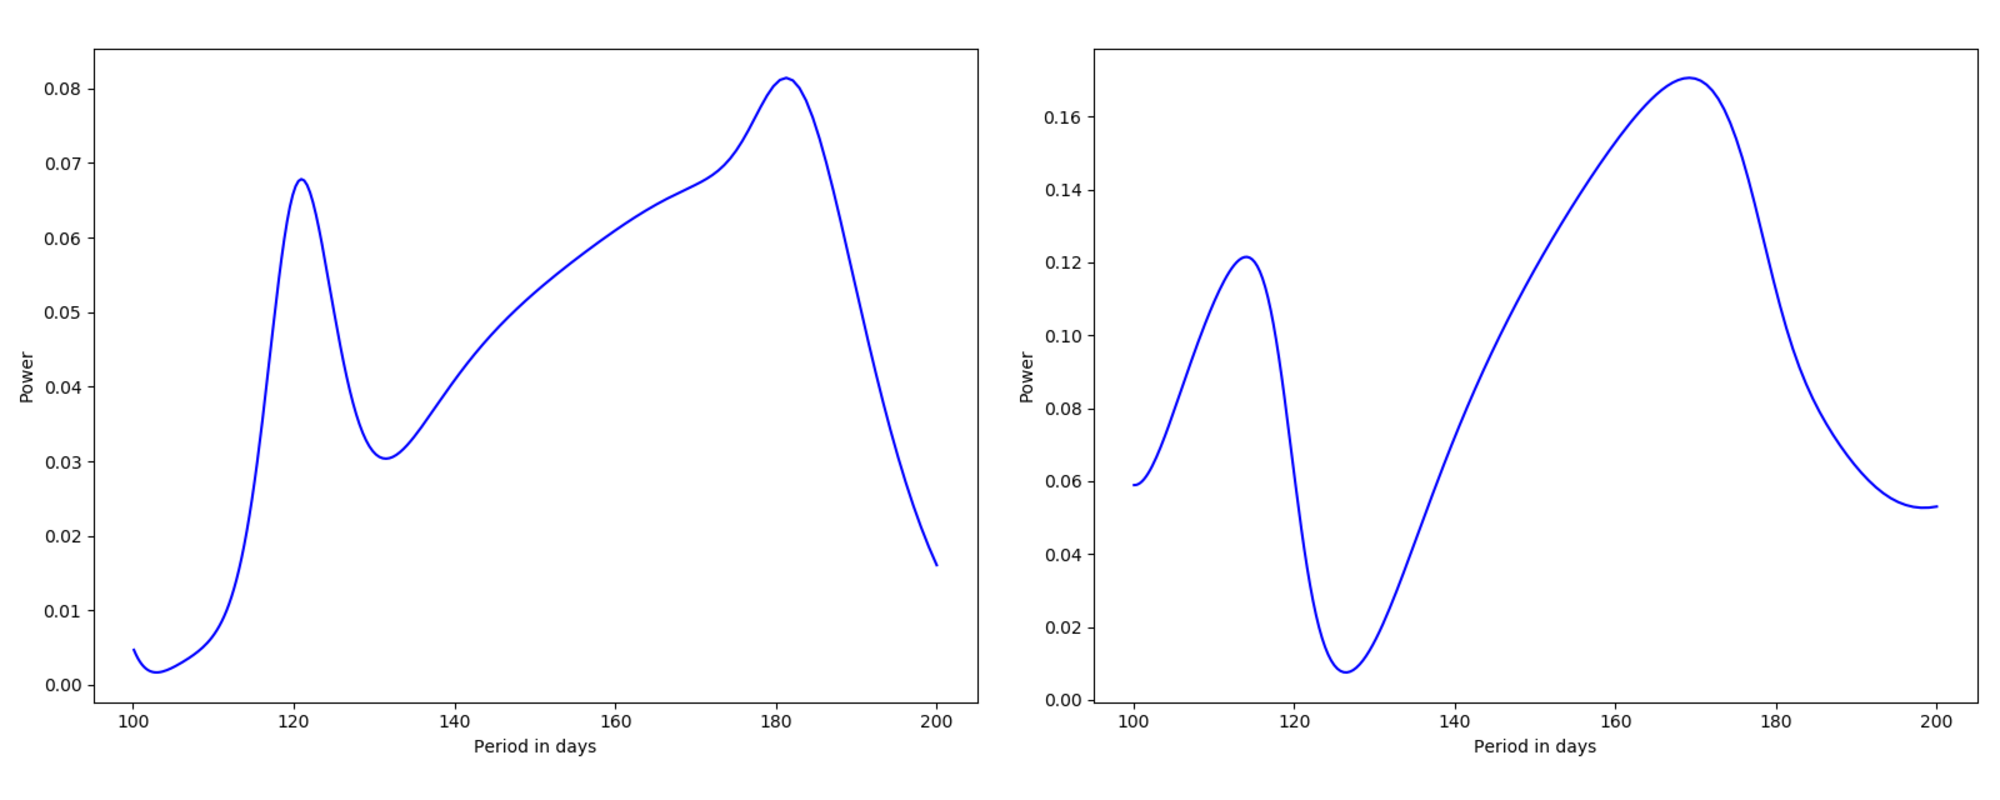
\includegraphics[scale=0.25]{images/ls123both.png}
% \end{center}   
% \caption{Periodograms obtained from Fig. \ref{fig:allref123}, left panel and Fig. \ref{fig:allref123bin} in right
%   panel. Only the \textbf{g} filter was used in this plot, the one from the \textbf{r} filter being almost identical.}
%   \protect\label{fig:ls123both}
% \end{figure}
% 
% \begin{figure}[!htbp]
% \begin{center}
% 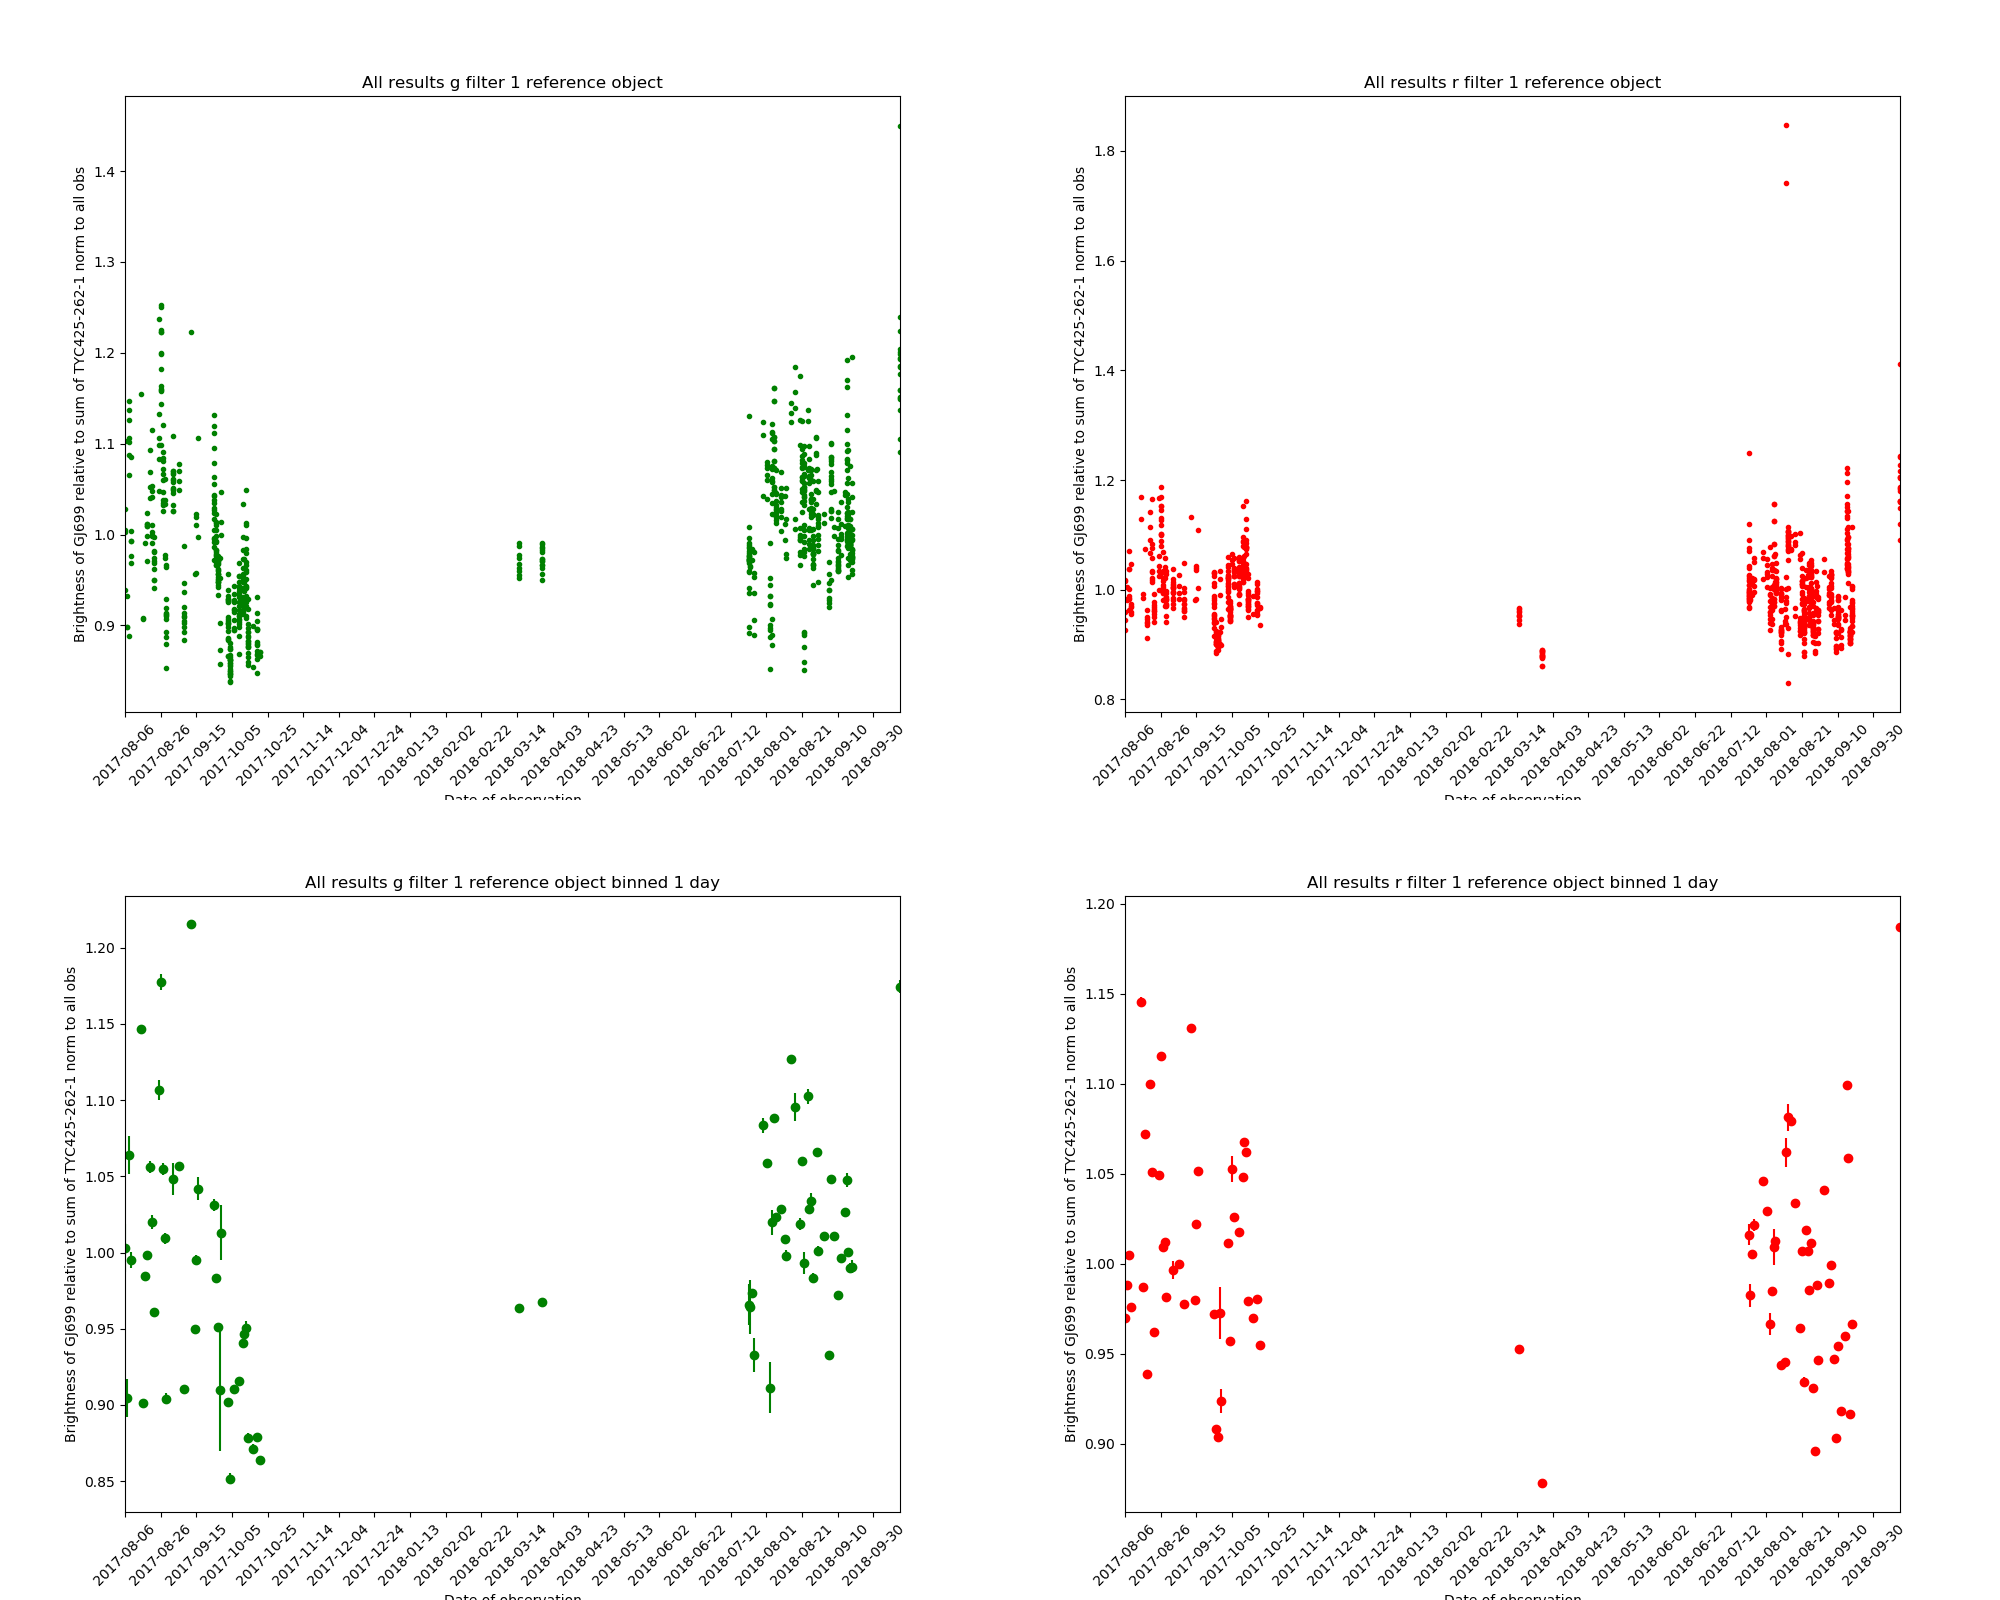
\includegraphics[scale=0.25]{images/allref1.png}
% \end{center}   
% \caption{This shows the ratio of the flux for the target, \bstar, to the strongest of the reference objects, TYC425-262-1.}
%   \protect\label{fig:allref1}
% \end{figure}
% 
% \begin{figure}[!htbp]
% \begin{center}
% 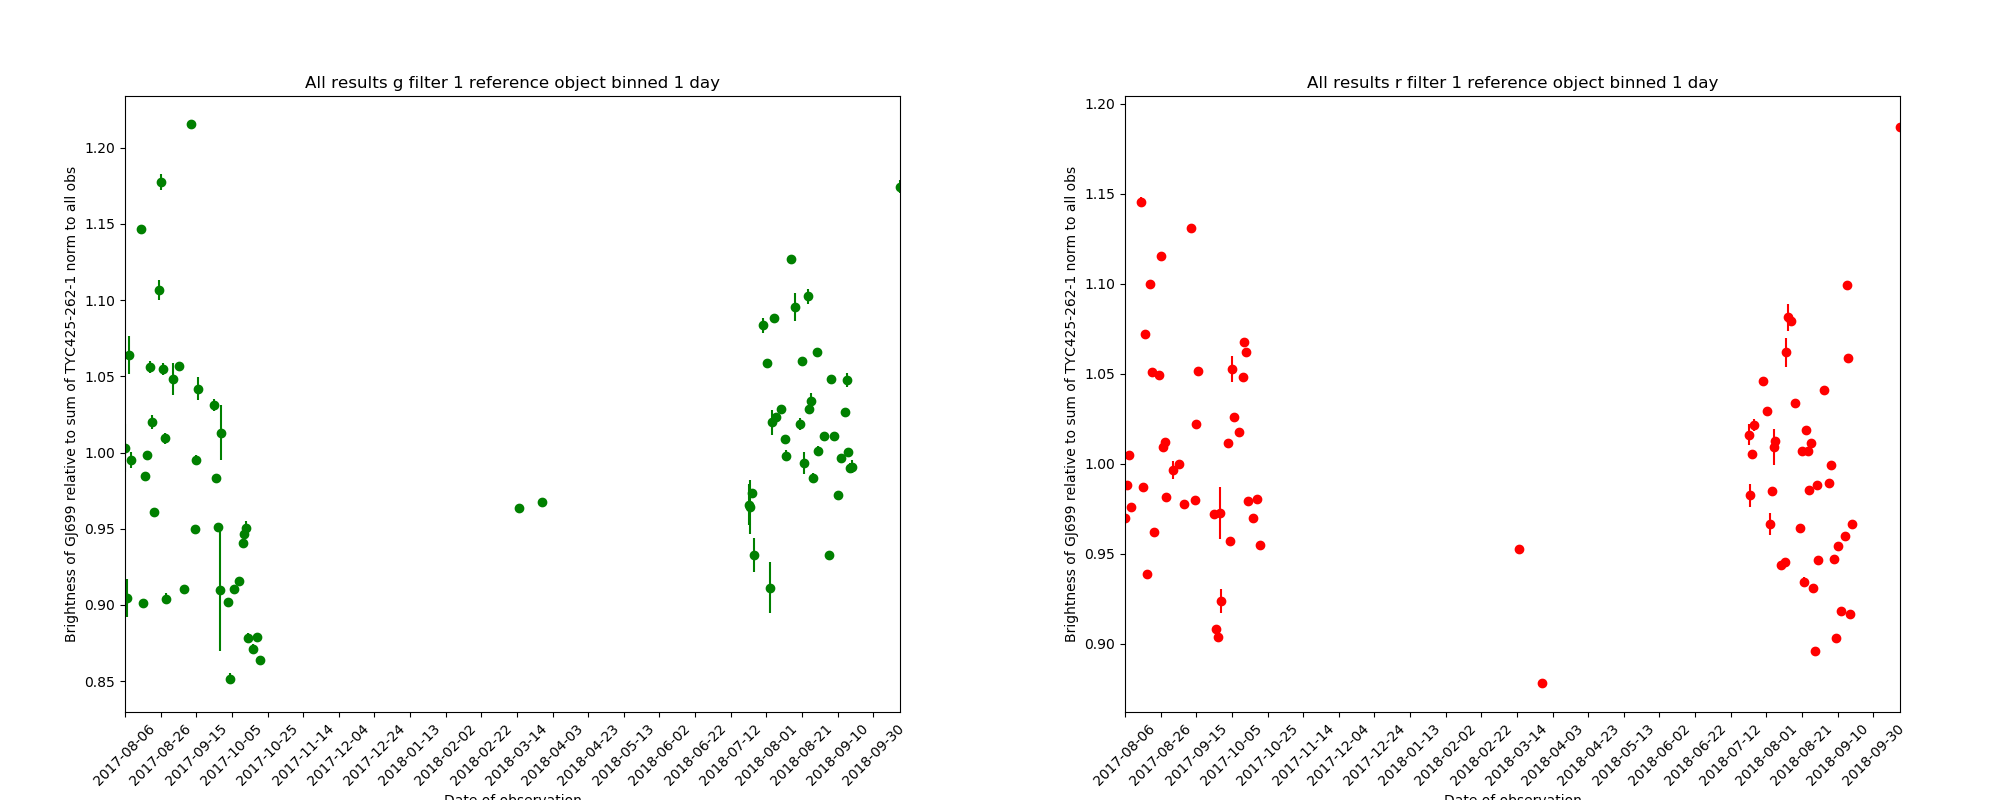
\includegraphics[scale=0.25]{images/allref1bin.png}
% \end{center}   
% \caption{This shows the ratio of the flux for the target, \bstar, to the strongest of the reference objects,
%   TYC425-262-1 per Fig. \ref{fig:allref1} and binned to 1 day.}
%   \protect\label{fig:allref1bin}
% \end{figure}
% 
% \begin{figure}[!htbp]
% \begin{center}
% 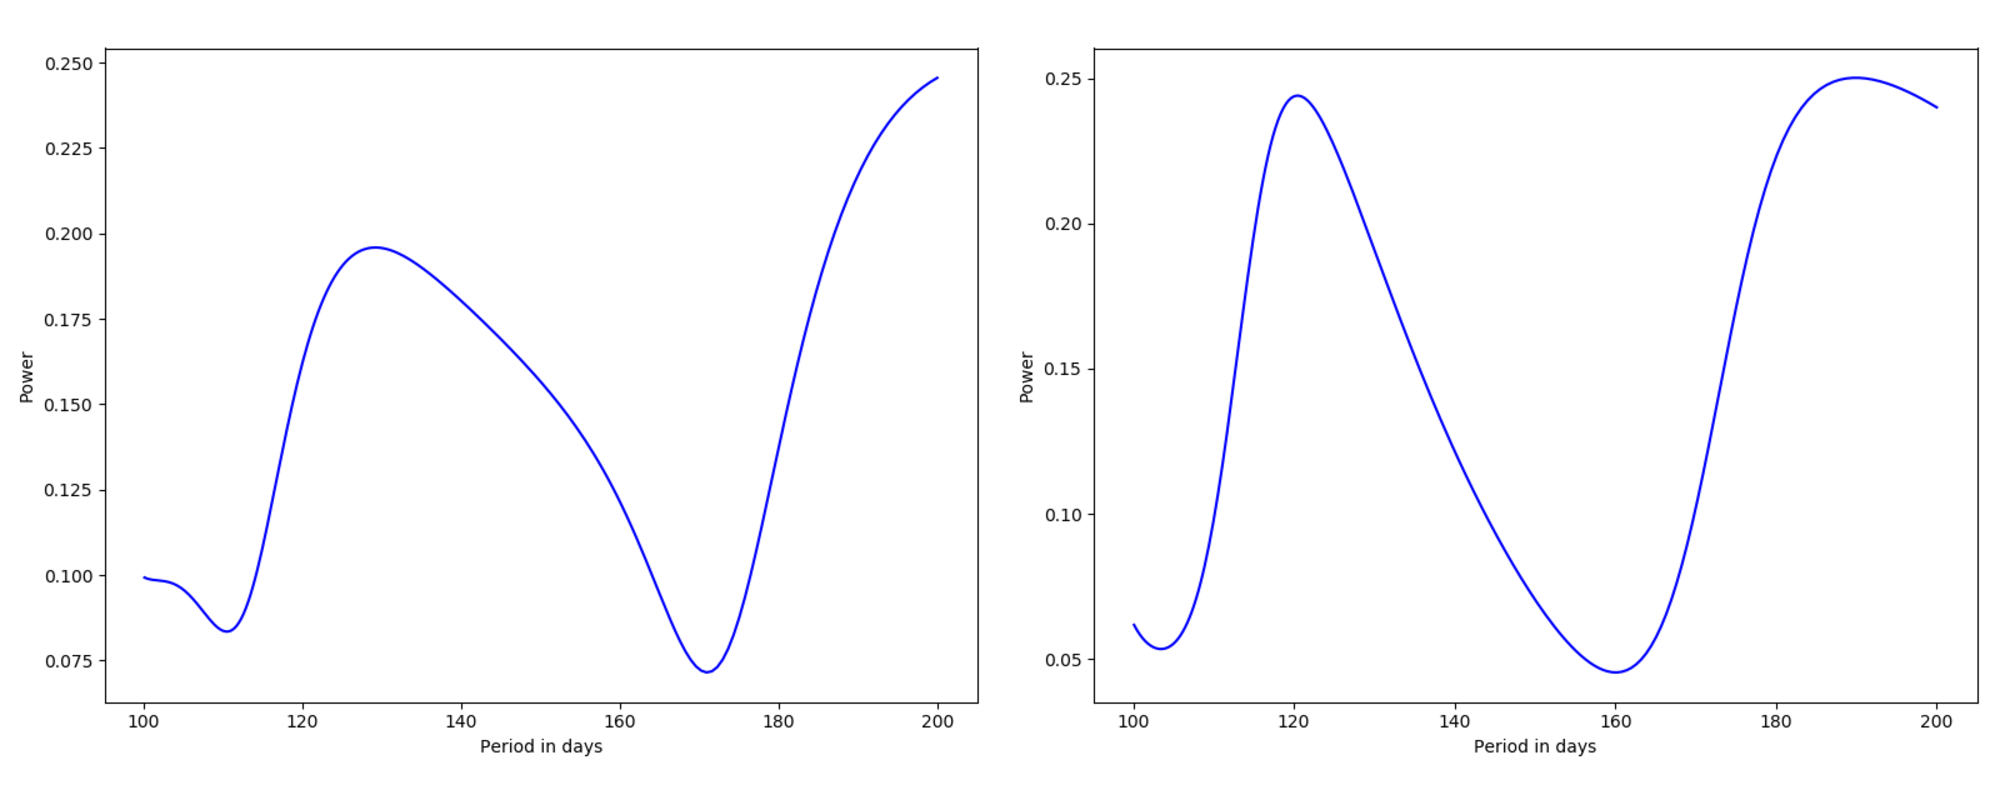
\includegraphics[scale=0.25]{images/ls1both.png}
% \end{center}   
% \caption{Periodograms obtained from Fig. \ref{fig:allref1}, left panel and Fig. \ref{fig:allref1bin} in right
%   panel. Only the \textbf{g} filter was used in this plot, the one from the \textbf{r} filter being almost identical.}
% \protect\label{fig:ls1both}
% \end{figure}
% \clearpage


%\section{Method and results}
\protect\label{section:results}

The following approach was taken to analyse the data.

Please note that much of this initial work was done with available data up to
the end of October 2018. There has been later date available in July 2019, but
the images and analysis below were propared before then.

\subsection{Intensity comparison}
\protect\label{section:intcomp}

As a first attempt to study the data, I took the ADU count, specifically the net after applying the flat and bias files
of the target in all the images in which it was available. The target was found in all of the images, apart from in some of the
\textbf{g}, \textbf{i} and \textbf{r} visible light filters, as shown in Table \ref{table:occtb} below.

Plotting light curves of the intensities obtained in this way yields Fig. \ref{fig:allall}.
Binning the intensities together into a single day gave
Fig. \ref{fig:allbin}, the error bars indicate the spread over a single day. I plotted
periodograms, as shown in Fig. \ref{fig:pgrams}. Despite the crudeness of the data, it is noticeable that there are
peaks close to the rotation periods of the order of 150 days referred to in \citet{suarezmascareno15} and \citet{toledopadron18}.

\begin{figure}[!htbp]
\begin{center}
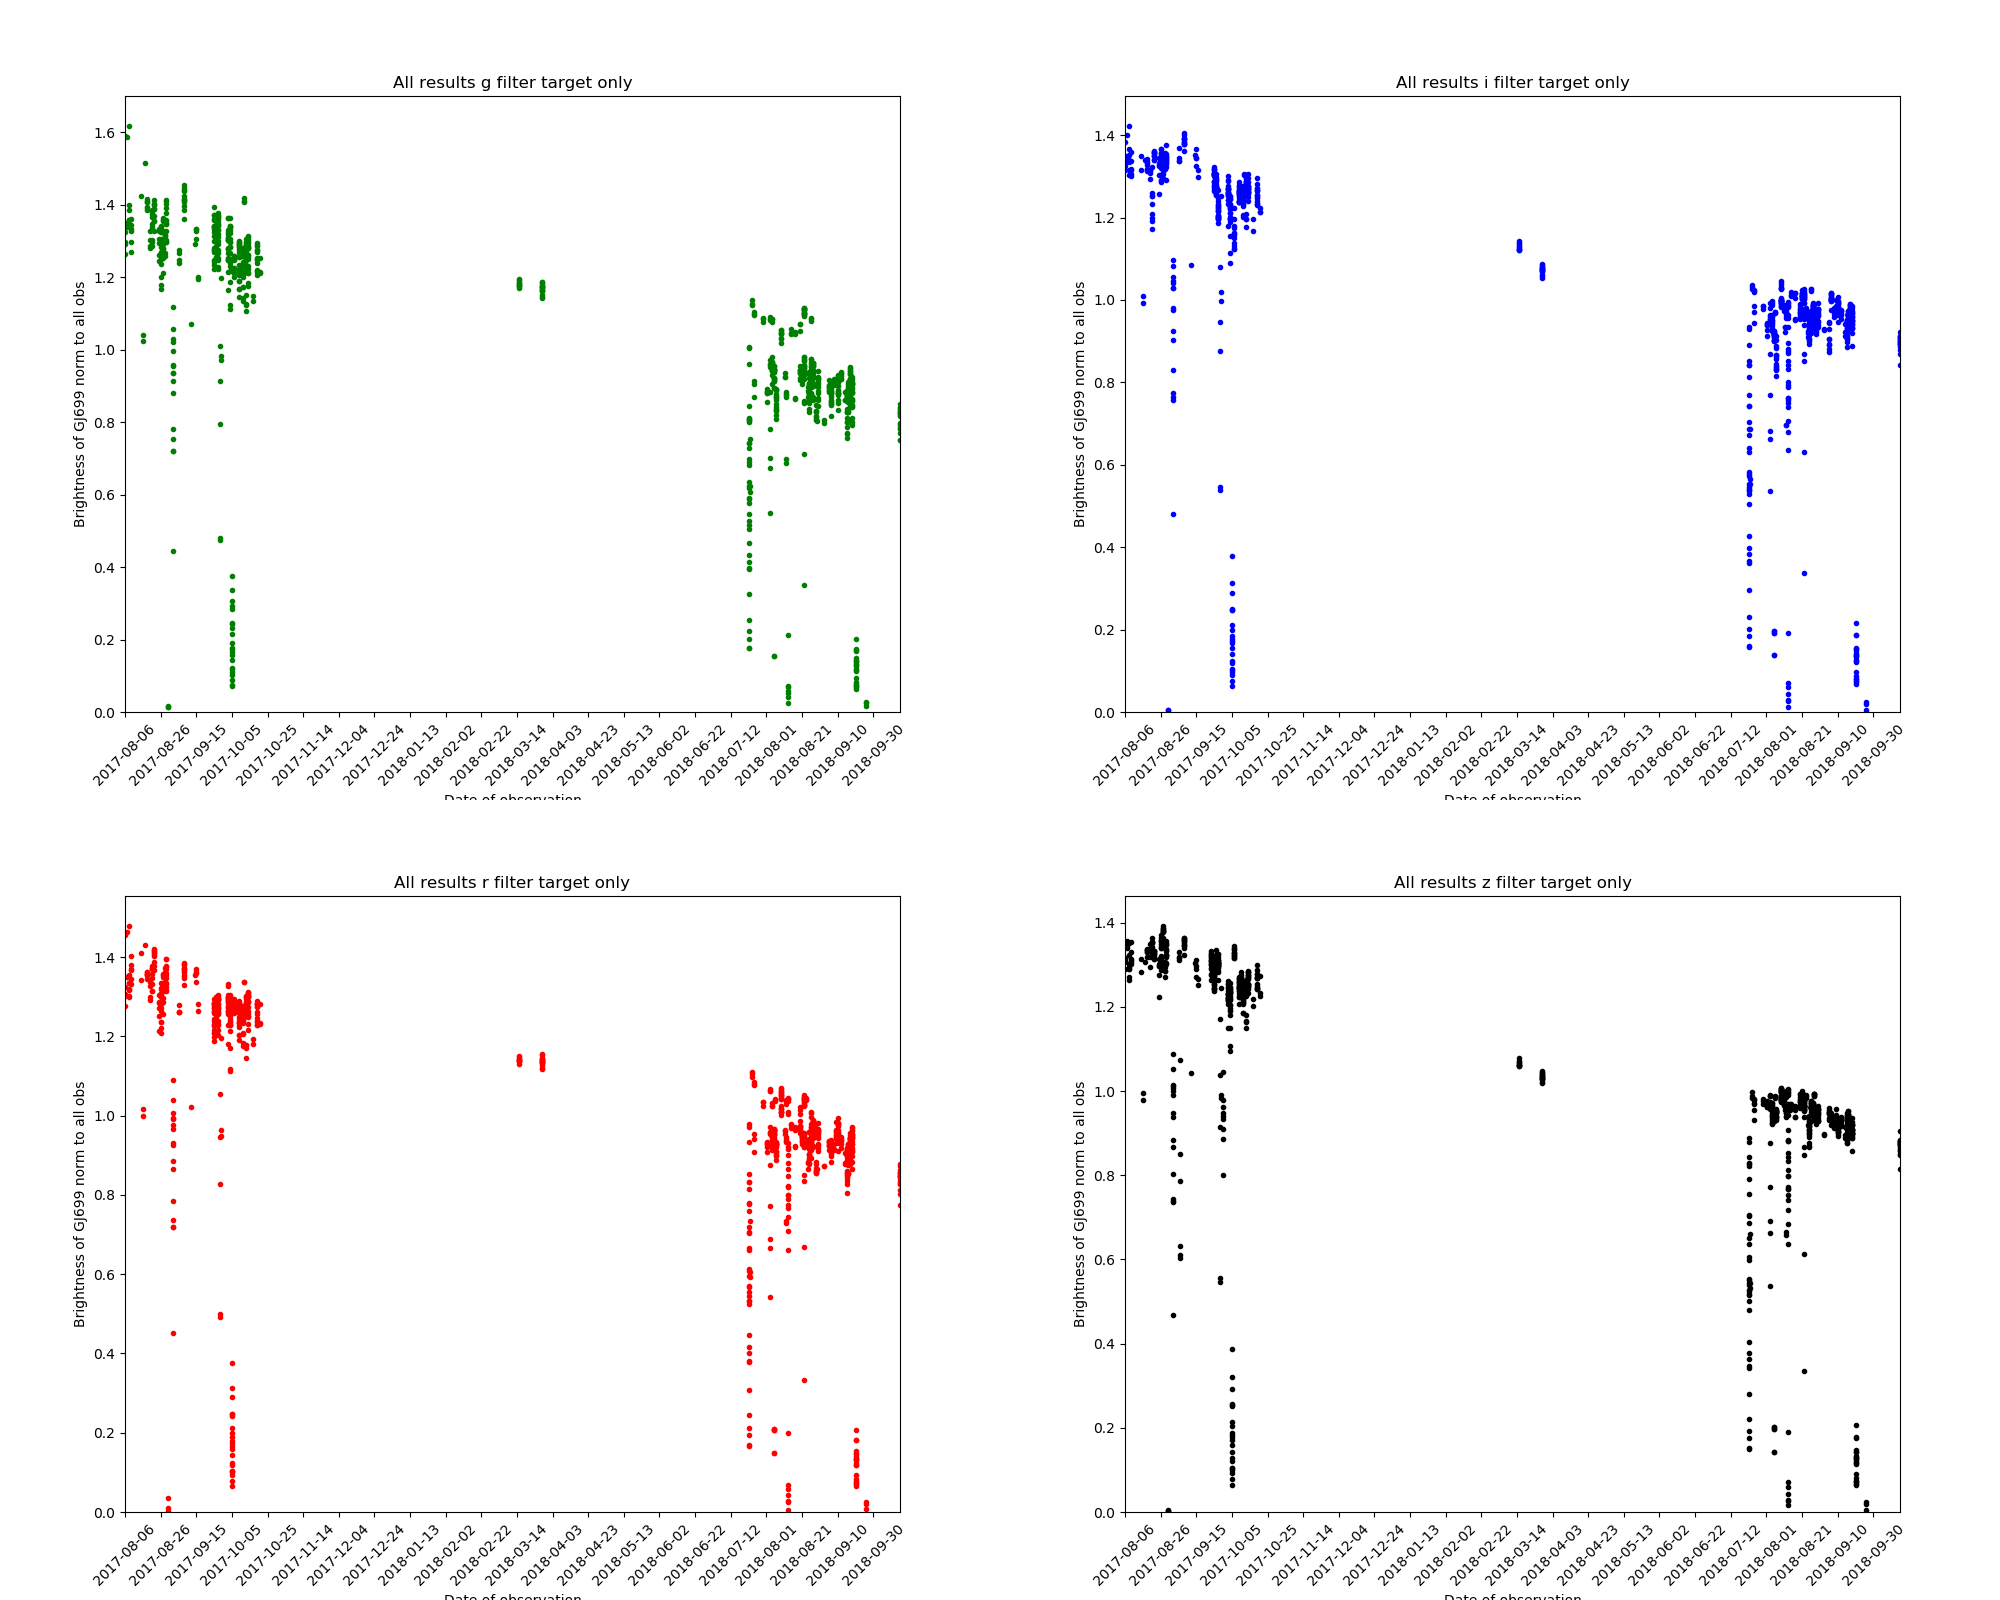
\includegraphics[scale=0.25]{images/allall.png} \\
\end{center}   
\caption{This shows the flux for the target, \bstar, for each of the four visible light filters. This takes the total
  ADU count only}
  \protect\label{fig:allall}
\end{figure}

\begin{figure}[!htbp]
\begin{center}
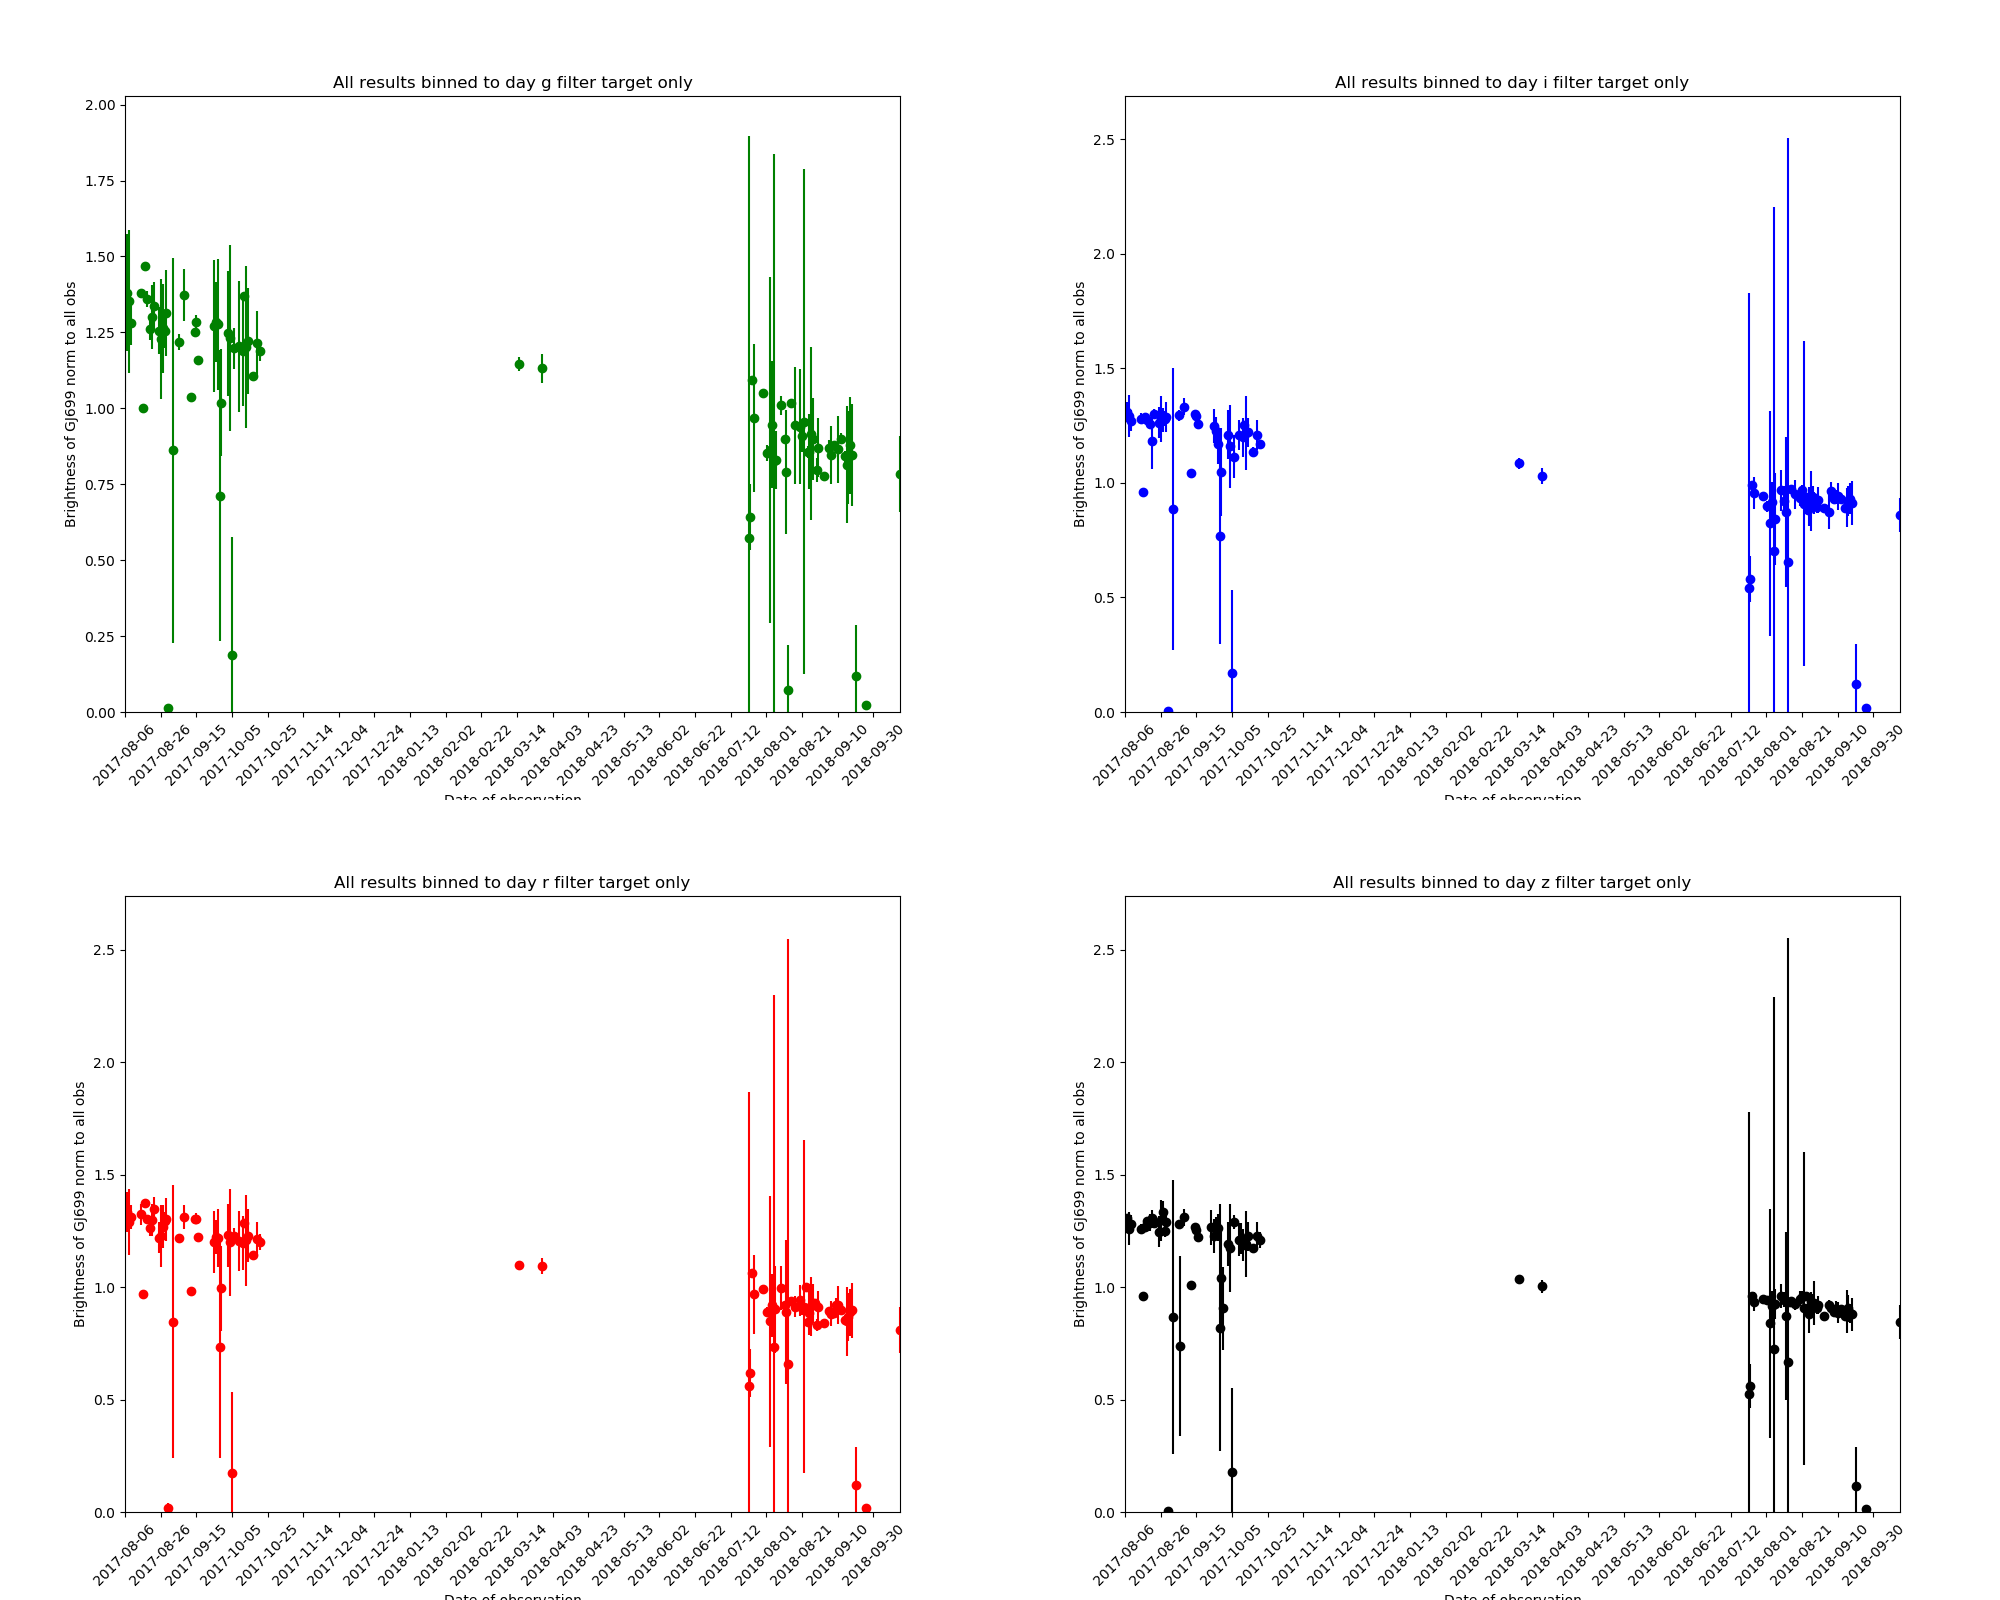
\includegraphics[scale=0.25]{images/allbin.png} \\
\end{center}   
\caption{This shows the flux for the target, \bstar, for each of the four visible light filters and binned to a single day. Error bars are show to indicate the spread of intensities over a single day.}
  \protect\label{fig:allbin}
\end{figure}

\begin{figure}[!htbp]
\begin{center}
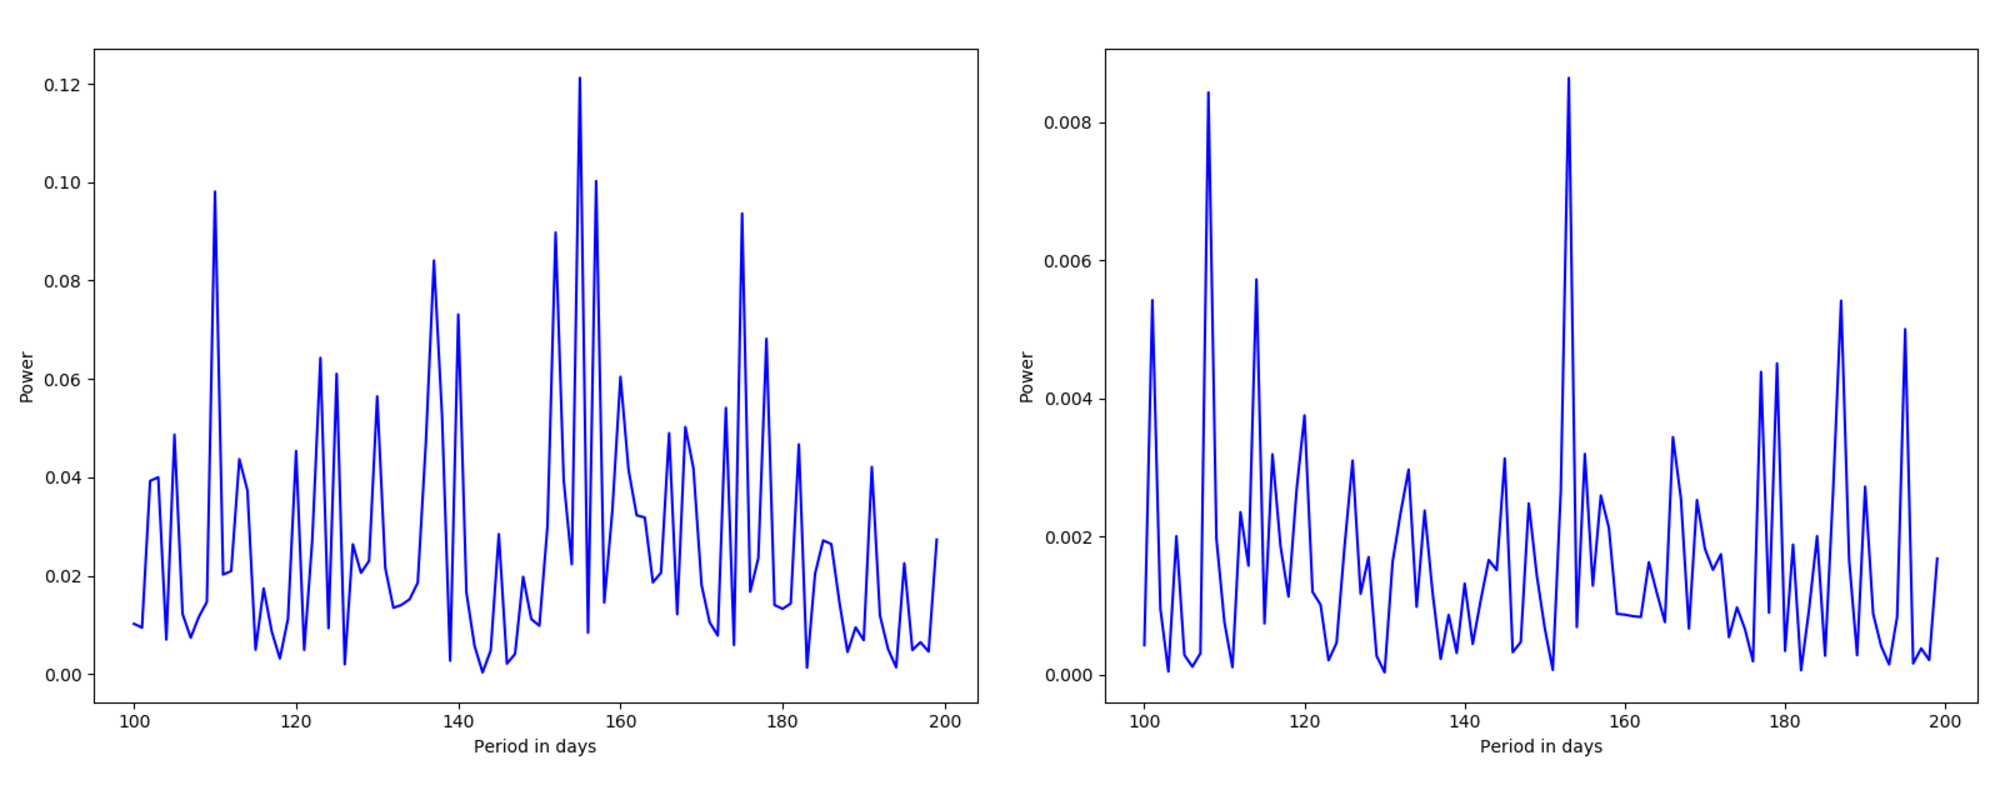
\includegraphics[scale=0.25]{images/pgrambunb.png} \\
\end{center}   
\caption{This displays periodograms derived from the binned (Fig. \ref{fig:allbin}) and unbinned
  (Fig. \ref{fig:allall}) light curves for the \textbf{r} filter.}
  \protect\label{fig:pgrams}
\end{figure}

It is accepted that this initial treatment is crude. Serious work needs to be done on correction for air mass,
which for a few observations, where they are spread over a period of several hours,
can be quite large, and to more accurately discard as unacceptable images with large or very variable sky levels.
There are some currently inexplicable variations, for
example the to images in Fig. \ref{fig:tyeg} give radically different ADU counts despite being taken two minutes apart
with same exposure time and other parameters.

\begin{figure}[!htbp]
\begin{center}
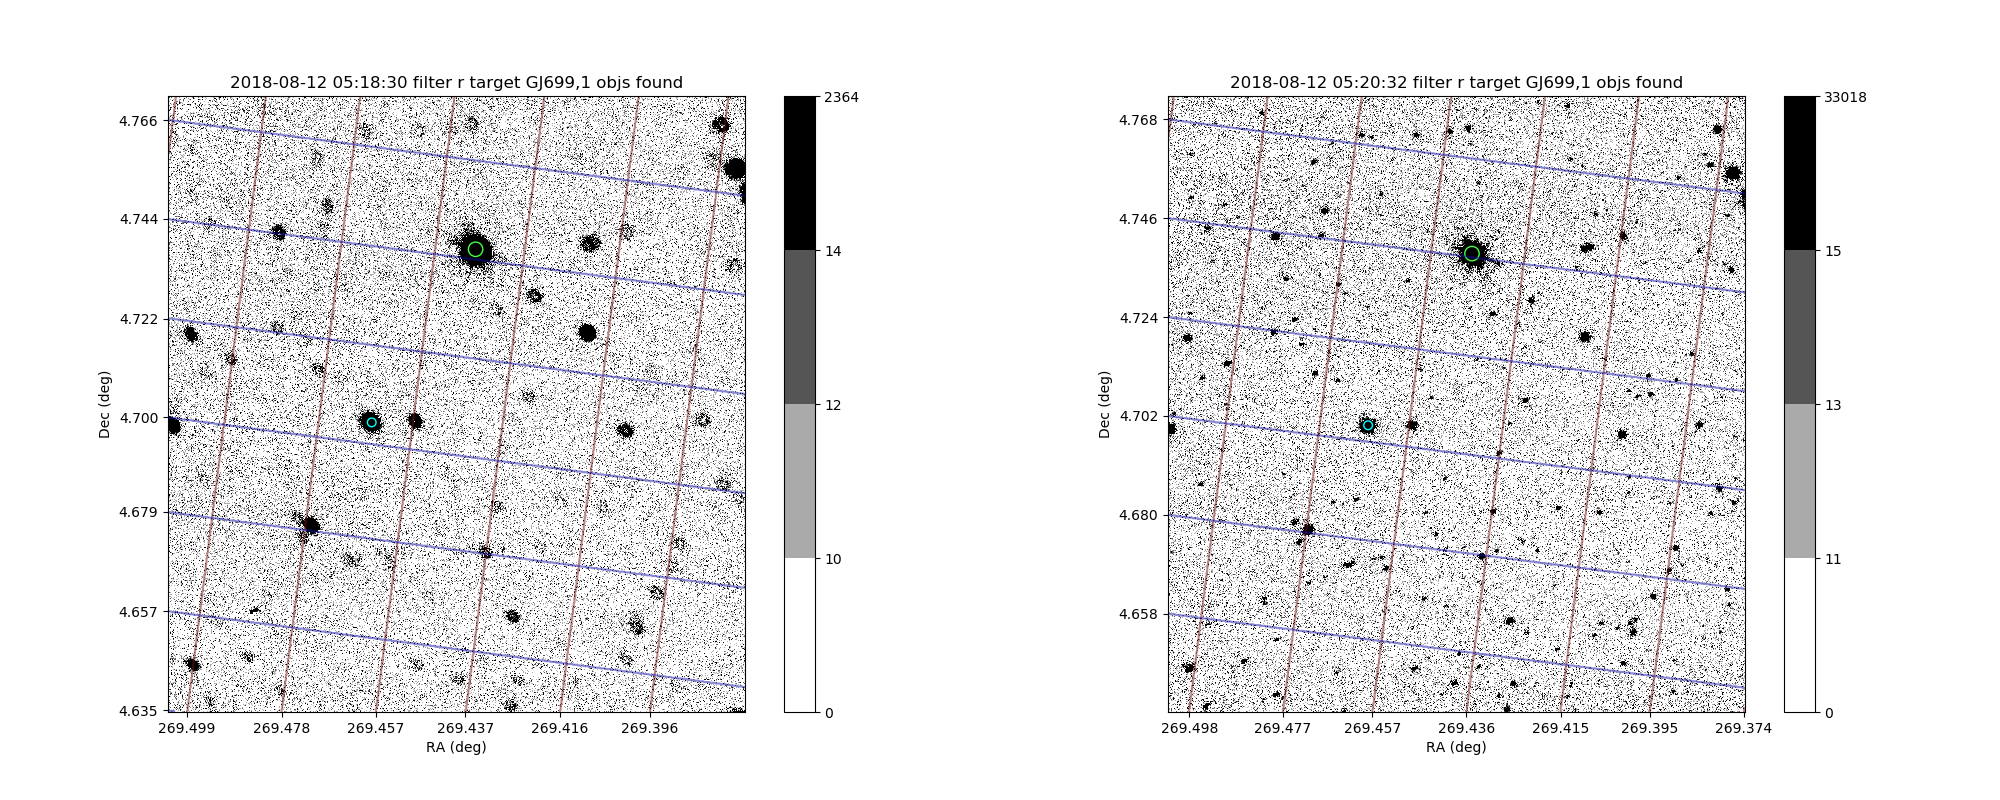
\includegraphics[scale=0.25]{images/tyeg.png}
\end{center}   
\caption{These images show an example of where 2 images taken 2 minutes apart with the same exposure time gave different flux values.}
  \protect\label{fig:tyeg}
\end{figure}

\subsection{Reference Stars}
\protect\label{section:refstars}

Rather than relying on the ``raw'' flux from the target star itself, I made an approach based on identified reference
stars found in a significant number of images. Ideally these should be as many as possible to ``smooth'' out errors and
variations on the reference star. By taking the ratio of the target star ADU count to the sum of the reference star
ADUs, then we can hope to achieve results for intensity with the factors such air mass corrections factored out, This
approach was taken in \citet{berry11} and would seem to involve least work, provided sufficient reference stars are
consistently found.

The algoritm used to find objects was first to locate the target (there was
usually a certain amount of error in the coordinates of the images) and then
find prefeviously-known reference objects. The criterion for finding objects was to look for groups of pixels within a
given scan aperture whose mean count was a given number of standard deviations
(intially 3) from that of the sky level. If the result appeared to be one of
the objects known already, the given reference object was deemed to have been
found.

To initialise the database of objects, I used Simbad, 2MASS and SDSS to find objects in the vicinity of \bstar, obtaining the following stars as shown in Table
\ref{table:reftimesfound}. Of the stars there, the types are unavailable apart from the most-frequently occurring one of
TYC425-262-1, which is an A3V star (this is also reported as the most frequently found reference star in \citet{berry11}).

\begin{table}[!htbp]
\begin{center}
\begin{tabular}{llr} \hline
Number & Object & Times found \\\hline
1 & TYC425-262-1 & 5,277 \\
2 & SDSS1237671695527248969 & 3,408 \\
3 & 2MASSJ17574653+0447466 & 3,297 \\
4 & SDSS1237668573088841773 & 840 \\
5 & TYC425-223-1 & 369 \\
6 & SDSS1237671695527249415 & 15 \\
\hline
\end{tabular}
\end{center}
\caption{This lists the identified reference objects near to {\bstar} and the number of times found in the available
  data. Note that this data relates to images up to the end of October 2018.}
\protect\label{table:reftimesfound}
\end{table}

I decided to consider only the first 3 reference objects, which are labelled 1, 2 and 3 for convenience in the
remainder of this report, as the appearances of the others were too infrequent to render them worthwhile.

\subsection{Classification of results}
\protect\label{section:classresults}

The images presented challenges in various respects. The visible light images are all at different orientations and with
the target in different places in the image, so not all the reference stars appear in all of the images. In some cases
the reference stars are just not bright enough to rise sufficiently above the sky level.

\begin{table}[!htbp]
\begin{center}
\begin{tabular}{lrrrr}
&Filter g&Filter i&Filter r&Filter z\\\hline
Target not found&167&80&105&0\\
No ref objs found & 84 & 1,003 & 53 & 1,085 \\\hline
Obj 1 (with or without others) & 834 & 0 & 925 & 0 \\
Obj 2 (with or without others) & 561 & 1 & 574 & 0 \\
Obj 3 (with or without others& 526 & 0 & 573 & 0 \\
Obj 1 only & 43 & 0 & 100 & 0 \\
Obj 2 only & 0 & 1 & 1 & 0 \\
Obj 3 only & 0 & 0 & 0 & 0 \\
Objs 1 and 2 (with or without 3) & 561 & 0 & 573 & 0 \\
Objs 1 and 3 (with or without 2) & 526 & 0 & 573 & 0 \\
Objs 2 and 3 (with or without 1) & 296 & 0 & 321 & 0 \\
Objs 1 and 2 only & 265 & 0 & 252 & 0 \\
Objs 1 and 3 only & 230 & 0 & 252 & 0 \\
Objs 2 and 3 only & 0 & 0 & 0 & 0 \\
Objs 1,2 and 3 & 296 & 0 & 321 & 0 \\
\hline
\end{tabular}
\end{center}
\caption{This table shows the occurrences of the 3 main reference objects in each of the observations with or without
  the others. The infrared images were omitted as no reference objects were found in any of them. Note however the lack
  of occurrences of reference objects in the \textbf{i} and \textbf{z} filter images.}
\protect\label{table:occtb}
\end{table}

\subsection{Results from reference object comparisons}
\protect\label{section:refobjres}

Repeating the light curve plots from Section \ref{section:intcomp}, this time as the ratio of the ADU count of the
target to the sum of the first three reference objects, Fig.  \ref{fig:allref123} and Fig. \ref{fig:allref123bin} show
the light curves for the \textbf{r} and \textbf{g} filters. Also shown in Fig. \ref{fig:ls123both} are periodograms
derived from these light curves. Also shown in Fig \ref{fig:allref1}, Fig. \ref{fig:allref1bin} and Fig. \ref{fig:ls1both}
are the corresponding results taking into account only the brightest of the reference objects, TYC425-262-1.

\begin{figure}[!htbp]
\begin{center}
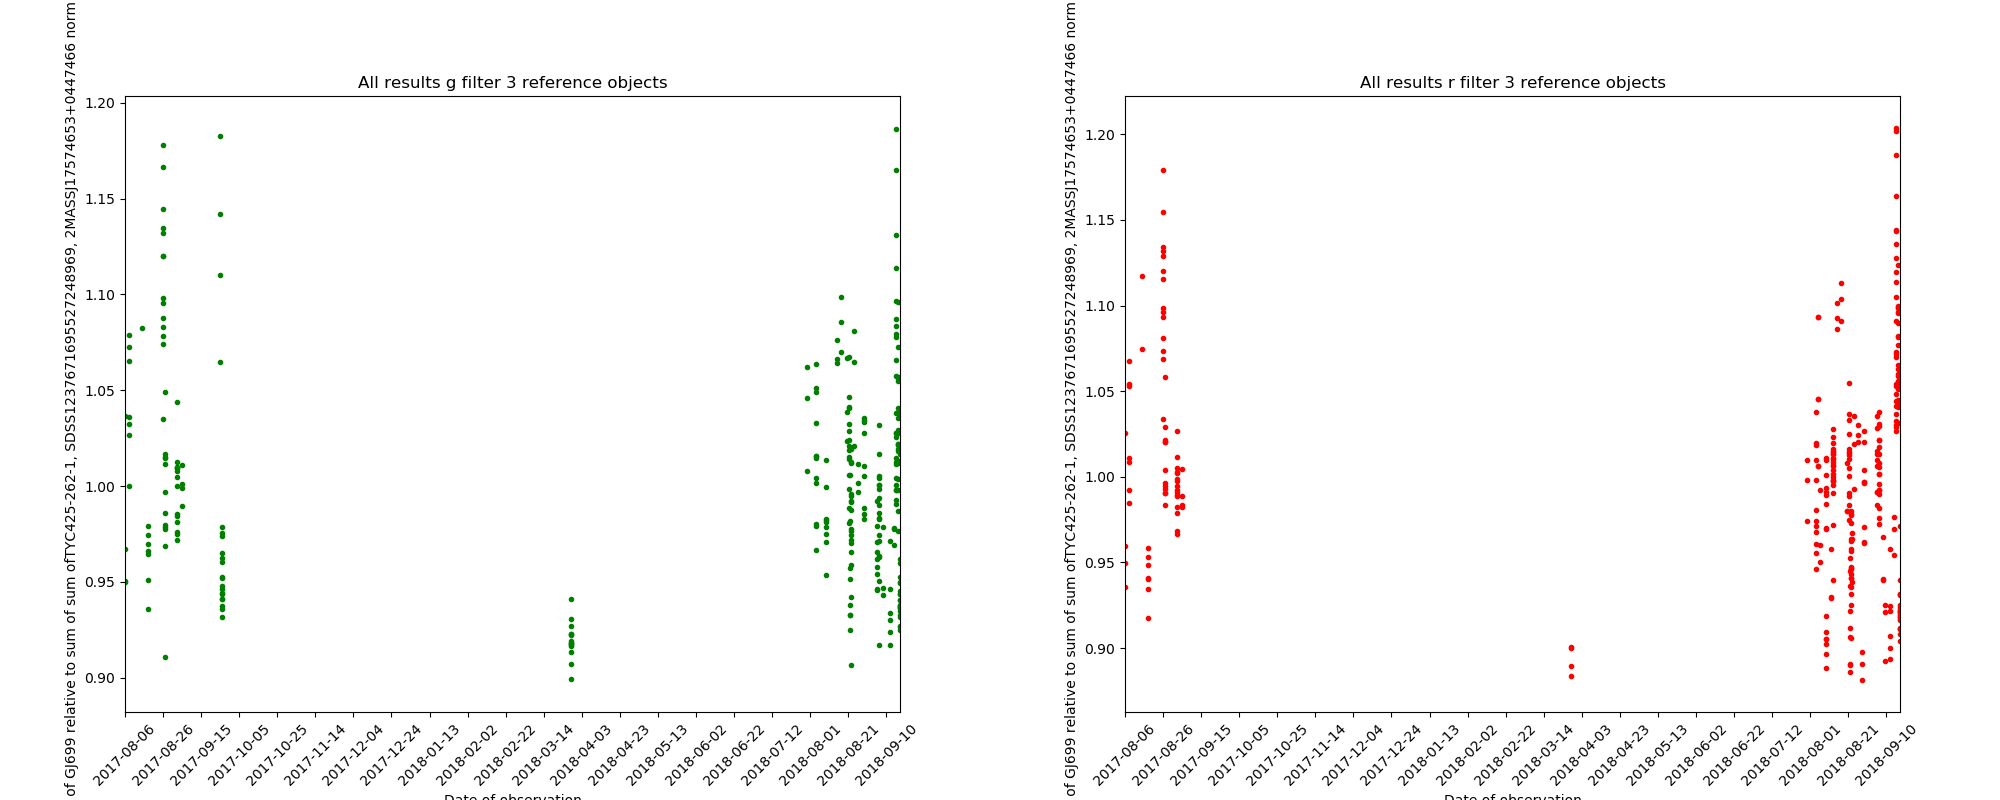
\includegraphics[scale=0.25]{images/allref123.png}
\end{center}   
\caption{This shows the ratio of the flux for the target, \bstar, to the 3 main reference objects for the \textbf{g} and
\textbf{r} filters, plotted as green and red respectively.}
  \protect\label{fig:allref123}
\end{figure}

\begin{figure}[!htbp]
\begin{center}
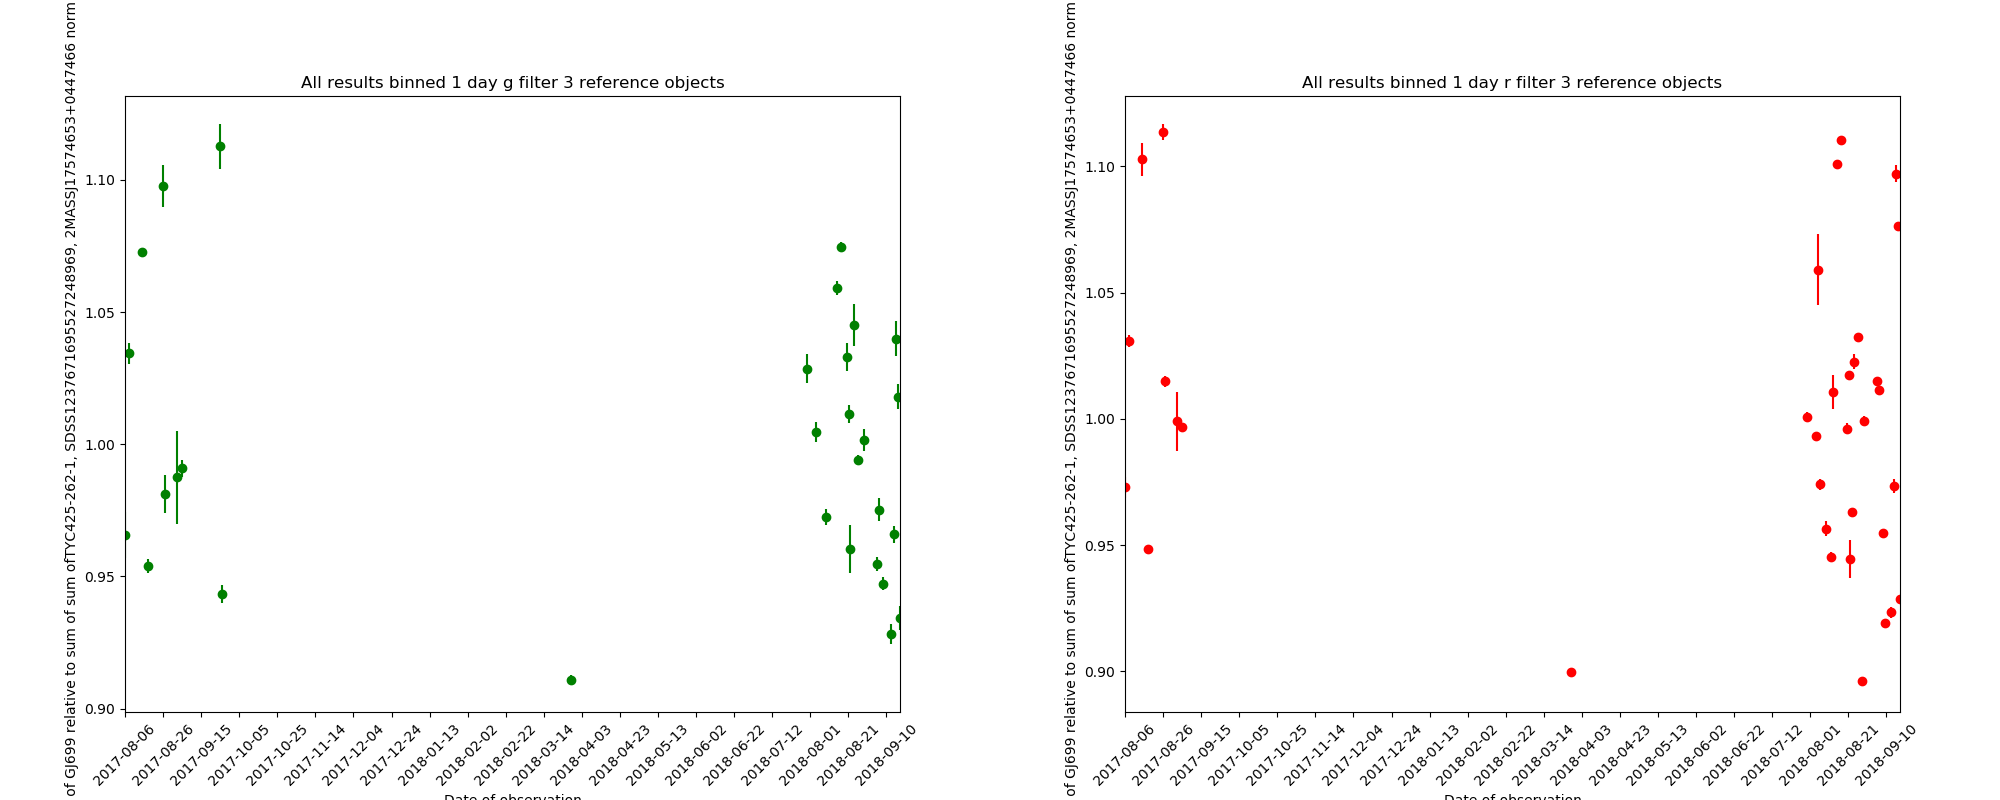
\includegraphics[scale=0.25]{images/allref123bin.png}
\end{center}   
\caption{This shows the ratio of the flux for the target, \bstar, to the 3 main reference objects as per Fig. \ref{fig:allref123} and binned to 1 day.}
  \protect\label{fig:allref123bin}
\end{figure}

\begin{figure}[!htbp]
\begin{center}
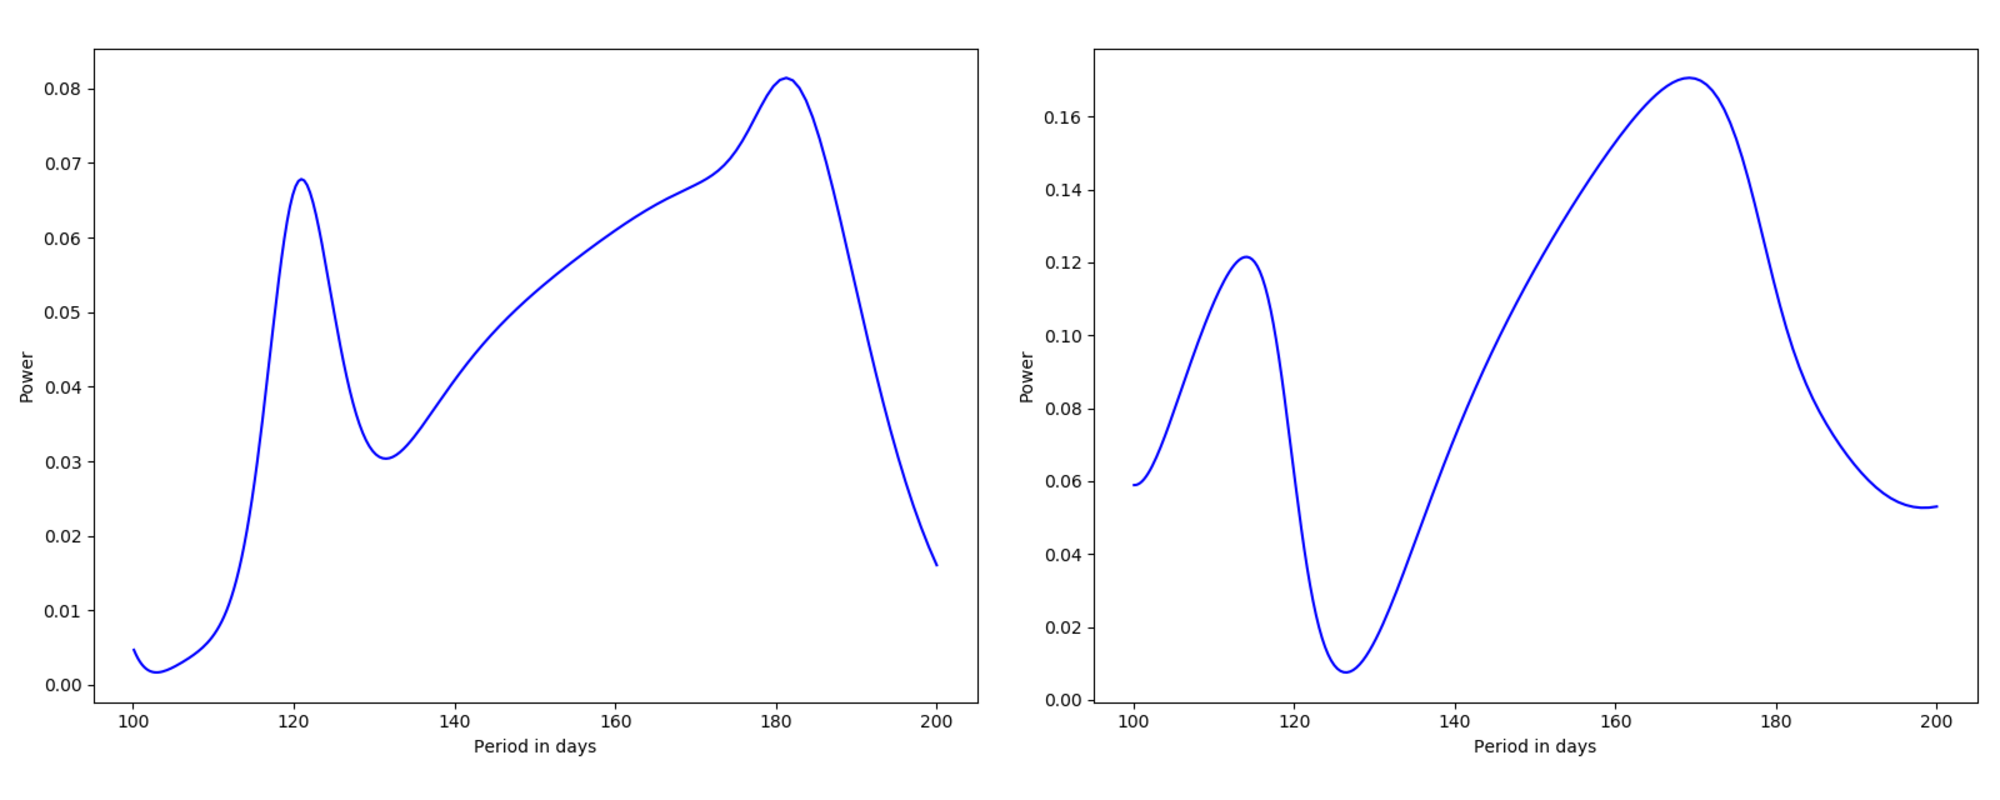
\includegraphics[scale=0.25]{images/ls123both.png}
\end{center}   
\caption{Periodograms obtained from Fig. \ref{fig:allref123}, left panel and Fig. \ref{fig:allref123bin} in right
  panel. Only the \textbf{g} filter was used in this plot, the one from the \textbf{r} filter being almost identical.}
  \protect\label{fig:ls123both}
\end{figure}

\begin{figure}[!htbp]
\begin{center}
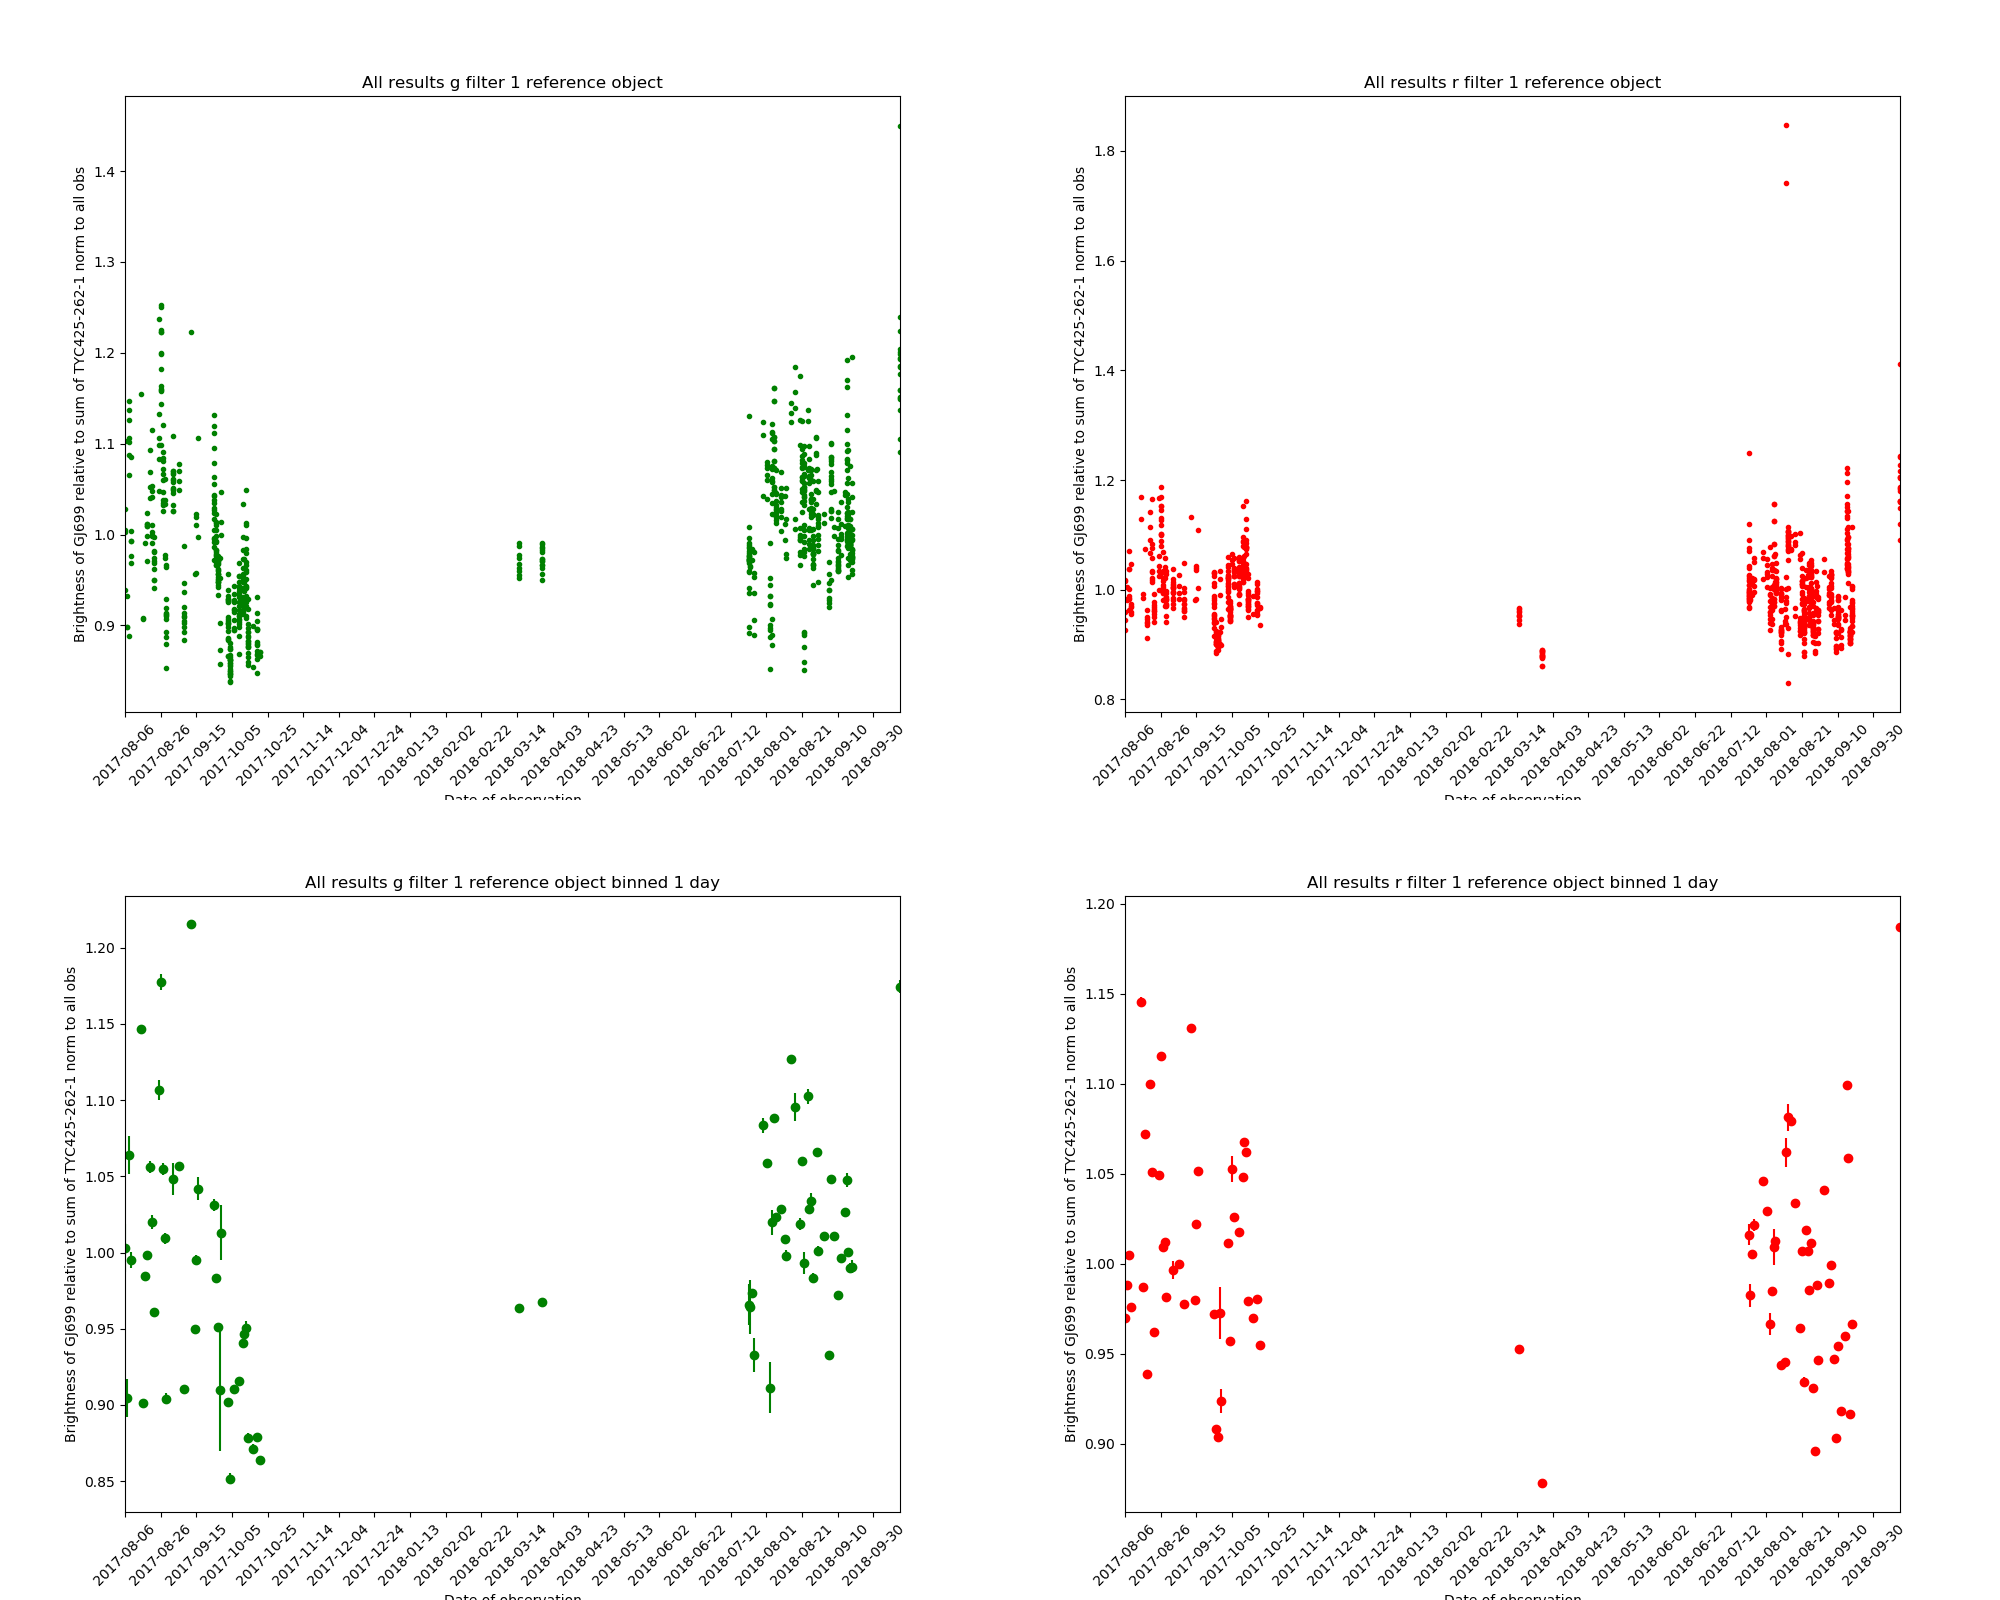
\includegraphics[scale=0.25]{images/allref1.png}
\end{center}   
\caption{This shows the ratio of the flux for the target, \bstar, to the strongest of the reference objects, TYC425-262-1.}
  \protect\label{fig:allref1}
\end{figure}

\begin{figure}[!htbp]
\begin{center}
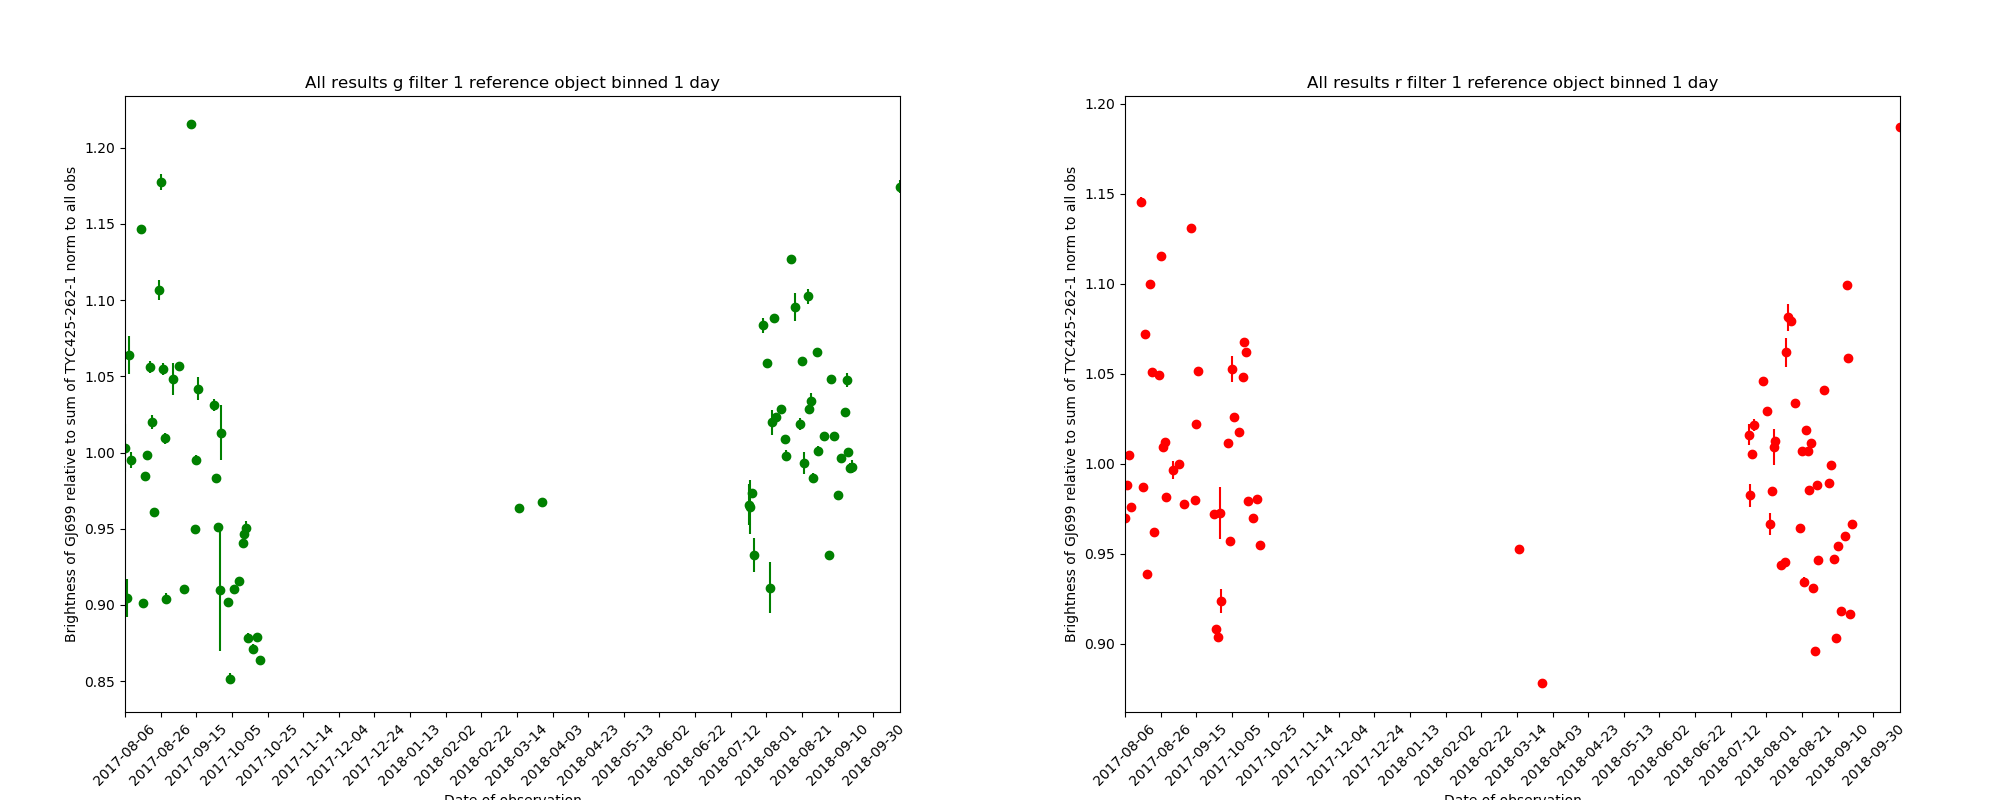
\includegraphics[scale=0.25]{images/allref1bin.png}
\end{center}   
\caption{This shows the ratio of the flux for the target, \bstar, to the strongest of the reference objects,
  TYC425-262-1 per Fig. \ref{fig:allref1} and binned to 1 day.}
  \protect\label{fig:allref1bin}
\end{figure}

\begin{figure}[!htbp]
\begin{center}
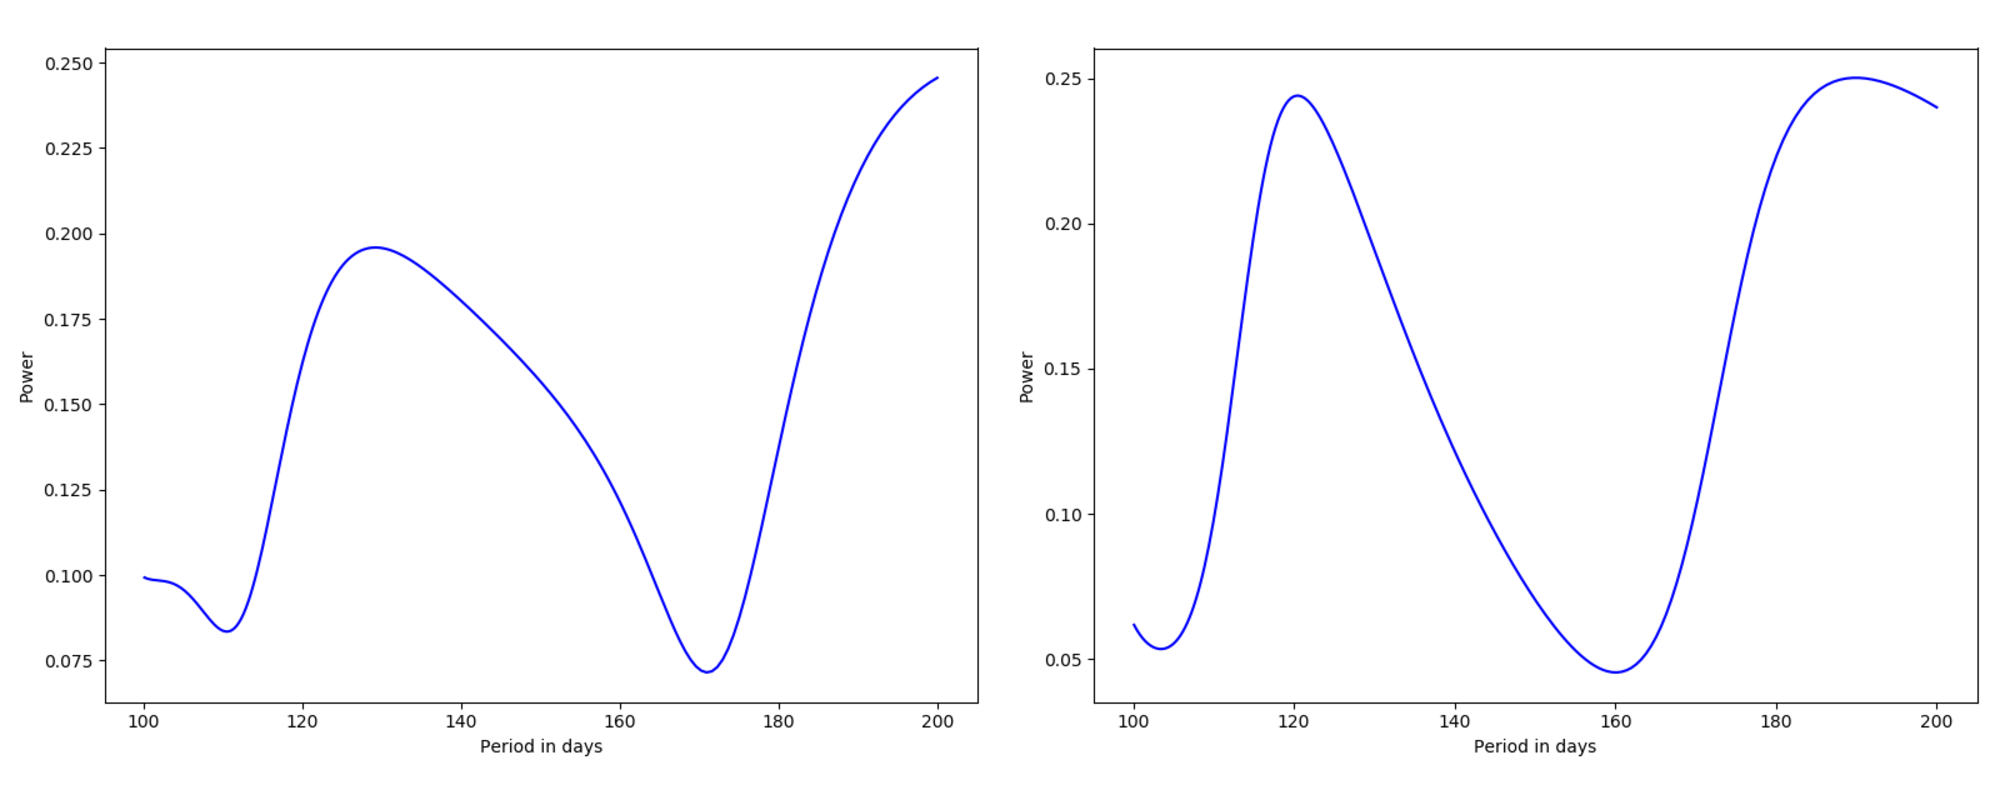
\includegraphics[scale=0.25]{images/ls1both.png}
\end{center}   
\caption{Periodograms obtained from Fig. \ref{fig:allref1}, left panel and Fig. \ref{fig:allref1bin} in right
  panel. Only the \textbf{g} filter was used in this plot, the one from the \textbf{r} filter being almost identical.}
\protect\label{fig:ls1both}
\end{figure}
\clearpage

%\section{Further work}
\protect\label{section:worktocome}

The following is the programme of work I need to undertake to ready the project
to a state where serious science can be achieved.

In all cases, the work to be done will need revisiting and refining and
``iterating until convergence'' achieved.

\subsection{Completion and improvement of work to date}
\protect\label{section:fwimprovecompletion}

This currently documents work in progress and the following needs to be achieved
or at least an initial version complete before the project is ready to move
forward.

\subsubsection{Completion of revised calibration}
\protect\label{section:fwcalib}

I need to put together the work on revised bias and flat files, also of bad
pixel identification, so as to minimise the loss of useful data, refining whether
to discard a pixel altogether or assign a low weighting.

Some parts, especially of limits to flat fields, may not be needed; there is
plenty of scope for refinement.

Also needed is a reasonable assessment of the uncertainty of any measurements
taken.

I need to insert new versions of Fig. \ref{fig:initgexample} and following
into this report in section \ref{section:postcalibration} showing improvements
made.in these fields, with a first version ready by the end of the first week in
June 2022.

\subsubsection{Revise identification of objects other than targets}
\protect\label{section:fwtargets}

I populated the database of objects from SIMBAD and GAIA EDR3 in May 2021 and
this needs revising. Some of the objects are closer to each other than the
resolution of the telescope, about 0.6 arc-seconds per pixel, can distinguish.

The identification of close objects is currently slightly random due to the
different orientations of the images and the order in which the search
algorithm takes sources. It may be that there are larger common subsets of
reference objects than are currently apparent. It may well be feasible to
regard close objects as a composite object for the purposes of using as
reference objects.

This will need doing with some care and I would hope to be confident of the
results for at least {\prox} by the end of June 2022.

\subsubsection{Optimise apertures and determine magnitudes and variability of
reference objects} \protect\label{section:fwoptap}

In order to evaluate magnitudes over all the images, it is necessary to have
confidence in the reference objects available in all of the images, rather than
the common subset of objects which appears in all images, which becomes
vanishingly small, especially for {\ross} and {\bstar} and for the \texttt{i}
and \texttt{z} filters.

This will need running through and comparing each object with each other object,
this is more of a processing issue than anything.

It would be desirable to build a picture of variability and compare this with the
variability statistics from other sources, so that an uncertainty figure can
be made for each target.

Also needed is a standard optimised aperture size for calculation of the
brightness of objects in any given image.

Although this is a highly iterative process, I should hope to have a ``first
pass" of this complete by mid-August 2022.

\subsection{Extraction of data}
\protect\label{section:fwextract}

The whole object is to obtain believable light curves and observational data
from the REM image data including values for uncertainty in which it is possible
to have confidence and this is what I intend to present by the end of September
2022.

Obtaining periodic data is particularly important and a clear objective of this
study would be to try to obtain this for \ross, (and consequently the
inclination angle) although as discussed in Section \ref{section:introross}. with a maximum
period of $3.5 \pm 1.5$ days, but with observation days months apart as shown in Fig. \ref{fig:rdwarfhist}, there will
be a considerable number of aliases to contend with.

Obviously too, an increase in the understanding of activity cycles of all three
main targets will hopefully be a useful consequence of this.

\subsection{Calculation of Barycentric dates, periodograms}
\protect\label{section:fwbarycentric}

Barcycentric dates need to be computed and inserted into the observation records
before periodograms can be extracted. Then need to start producing periodograms
of the data.

\subsection{Variations and improvements}
\protect\label{section:fwvariations}

There are a substantial number of choices made in the analysis of the data and
scope for seeing whether improvements in the accuracy can be brought about by
tuning some of them. In mind are:

\begin{enumerate}
  \item Using a weighted sum in calculating peaks as opposed to summing the ADUs
  and calculating the error.
  \item Using sub-standard images with weightings.
  \item Experiment with weightings of areas round the edges of the images, where
  vignetting and other effects affect the exposures.
  \item Using different sized apertures with different filters.
  \item Selection of different reference objects with different filters.
  \item Asking for changes to the exposure times.
  \item Plotting of periods of other objects found in the frames.\footnote{It
  might be necessary to revise the Barycentric dates in these cases but the
  ones for the targets will probably be accurate enough, but must check.}
\end{enumerate}

\subsection{Incorporation of other data}
\protect\label{section:fwincorp}

There is a complete set of REMIR data taken simultaneously with all the other
options, with calibration already done. It would be wasteful not to make
maximums use of this for comparison and for incorporation into the results where
possible.

Reference object sets are a little more limited with these as the {\rdwarf}
targets are so much brighter in the Infrared compared to the others.

I also intend to look at other datasets and where possible undertake a similar
task with these.

\clearpage


\bibliographystyle{apj}
\bibpunct{(}{)}{;}{s}{,}{,}
\bibliography{bibrefs}

\protect\label{lastpage}
\end{document}
